\documentclass[times,english,brazil,oneside, a4paper, fleqn]{ifes8}

\usepackage{pgfgantt}
\usepackage{graphicx}
\usepackage[utf8]{inputenc}


\usepackage[utf8]{inputenc}
\usepackage{lastpage}           % Usado pelo exemplo de ficha catalográfica
\usepackage[abnt-full-initials=yes, alf, abnt-doi=doi]{abntex2cite}
\usepackage{microtype}          % para melhorias de justificação
\usepackage{morefloats}         % permite mais floats
\usepackage{listings}
\usepackage{xcolor}
\usepackage{tikz}
\usetikzlibrary[topaths]
\usepackage{mathtools}
\usepackage[final]{pdfpages}
%\usepackage{caption}
\usepackage{subcaption}
\usepackage{multirow}
\usepackage{boxhandler}
\usepackage{todonotes}
\usepackage{placeins}
\usepackage{float}
\usepackage[export]{adjustbox}
\usepackage{tikz}

\definecolor{mygreen}{rgb}{0,0.6,0}
\definecolor{mygray}{rgb}{0.5,0.5,0.5}
\definecolor{mymauve}{rgb}{0.58,0,0.82}

%%% The \raggedbottom declaration makes all pages the height of the text on that page.
%%% No extra vertical space is added.
\raggedbottom

%%% Definição da linguagem padrão do documento (pacote babel) para
%%% definir que certas porções do texto (como o resumo, por exemplo)
%%% estão em uma língua estrangeira, usar as macros
%%% \foreignlanguage{languageB}{Text in another language}
%%% ou
%%% \begin{otherlanguage}{languageB}
%%% ...
%%% \end{otherlanguage}
\selectlanguage{brazil}
\setlength{\abovecaptionskip}{5pt} % espaçamento antes da legenda de tabelas/figuras

%%% Define que todos os códigos fontes construídos com o ambiente
%%% `lstlisting' terão uma borda simples.
\lstset{ %
  backgroundcolor=\color{white},   % choose the background color
  basicstyle=\footnotesize,        % size of fonts used for the code
  breaklines=true,                 % automatic line breaking only at whitespace
  captionpos=b,                    % sets the caption-position to bottom
  commentstyle=\color{mygreen},    % comment style
  escapeinside={\%*}{*)},          % if you want to add LaTeX within your code
  keywordstyle=\color{blue},       % keyword style
  stringstyle=\color{mymauve}, 
  numbers=left,
  stepnumber=1,    
  firstnumber=1,
  numberfirstline=true% string literal style,
   frame=top,frame=bottom, frame=single,
   captionpos=t,
   literate=
  {á}{{\'a}}1 {é}{{\'e}}1 {í}{{\'i}}1 {ó}{{\'o}}1 {ú}{{\'u}}1
  {Á}{{\'A}}1 {É}{{\'E}}1 {Í}{{\'I}}1 {Ó}{{\'O}}1 {Ú}{{\'U}}1
  {à}{{\`a}}1 {è}{{\`e}}1 {ì}{{\`i}}1 {ò}{{\`o}}1 {ù}{{\`u}}1
  {À}{{\`A}}1 {È}{{\'E}}1 {Ì}{{\`I}}1 {Ò}{{\`O}}1 {Ù}{{\`U}}1
  {ä}{{\"a}}1 {ë}{{\"e}}1 {ï}{{\"i}}1 {ö}{{\"o}}1 {ü}{{\"u}}1
  {Ä}{{\"A}}1 {Ë}{{\"E}}1 {Ï}{{\"I}}1 {Ö}{{\"O}}1 {Ü}{{\"U}}1
  {â}{{\^a}}1 {ê}{{\^e}}1 {î}{{\^i}}1 {ô}{{\^o}}1 {û}{{\^u}}1
  {Â}{{\^A}}1 {Ê}{{\^E}}1 {Î}{{\^I}}1 {Ô}{{\^O}}1 {Û}{{\^U}}1
  {œ}{{\oe}}1 {Œ}{{\OE}}1 {æ}{{\ae}}1 {Æ}{{\AE}}1 {ß}{{\ss}}1
  {ű}{{\H{u}}}1 {Ű}{{\H{U}}}1 {ő}{{\H{o}}}1 {Ő}{{\H{O}}}1
  {ç}{{\c c}}1 {Ç}{{\c C}}1 {ø}{{\o}}1 {å}{{\r a}}1 {Å}{{\r A}}1
  {€}{{\EUR}}1 {£}{{\pounds}}1
}

\newcommand{\ifestex}{\textsf{Ifes$8$}}
\newcommand{\specialcell}[2][c]{\begin{tabular}[#1]{@{}c@{}}#2\end{tabular}}

\titulo{Detecção e Diagnóstico Automatizado de Câncer de Pele utilizando Redes Neurais e Sistemas Multi-Agente}
\autor{Andrey Alexandre de Souza Basilio}
\local{Serra}
\data{2026}
\orientador[Orientador:]{Daniel Cruz Cavalieri}
\coorientador[Co-orientador:]{Cassius Zanetti Resende}
\instituicao{%
  Instituto Federal do Espírito Santo
 }
 \curso{Mestrado em Engenharia de Controle e Automação}
\tipotrabalho{Dissertação (Mestrado)}
% O preambulo deve conter o tipo do trabalho, o objetivo, 
% o nome da instituição e a área de concentração 
\preambulo{Dissertação apresentada à Coordenadoria do Curso de Mestrado em Engenharia de Controle e Automação do Instituto Federal do Espírito Santo, como requisito parcial para obtenção do título de Mestre em Engenharia de Controle e Automação.}



\begin{document}

\setsecnumformat{\csname the#1\endcsname\space}
\renewcommand{\afterchapternum}{\hspace{-4pt}}

%%% A macro \pretextual não precisa ser explicitamente chamada porque
%%% o abntex2 aciona essa macro no início do documento.
%%% \pretextual

\imprimircapa
\addtocounter{page}{-1}

\imprimirfolhaderosto*

\begin{fichacatalografica}
  \vspace*{\fill}
  % Posição vertical
  \begin{center}
    % Minipage Centralizado
    \fbox{
      \begin{minipage}[t]{12.5cm}
      será incluído ficha catalográfica fornecida pela biblioteca
      \end{minipage}
   }
  \end{center}
\end{fichacatalografica}
%\addtocounter{page}{-1}

% ------------------------- Folha de Aprovação ------------------------- 
\newpage
\begin{fichacatalografica}
  \begin{center}
    % Minipage Centralizado
    \fbox{
      \begin{minipage}[t]{14.5cm}
      \textbf{ASPECTOS QUE SE ESPERAM, SEJAM AVALIADOS PELA BANCA NO EXAME DE QUALIFICAÇÃO:}

\begin{enumerate}

\item \textbf{O problema da pesquisa foi formulado com clareza e a relevância de sua solução foi justificada?}

\item \textbf{Os objetivos foram bem definidos e claramente apresentados e são exequíveis no tempo disponível?}

\item \textbf{Há conexão clara entre a teoria apresentada e os objetivos da pesquisa?}

\item \textbf{A revisão do estado da arte foi realizada de forma a permitir a compreensão do contexto da pesquisa em relação ao que foi produzido até o momento?}
    
\item \textbf{A metodologia foi claramente descrita e atende aos objetivos propostos?}

\item \textbf{Os riscos da metodologia foram apresentados e as soluções propostas, são satisfatórias.}


\end{enumerate}

      
      %será incluída a folha de aprovação quando da defesa
      \end{minipage}
   }
  \end{center}
\end{fichacatalografica}
\newpage
% ------------------------- Folha de Aprovação ------------------------- 
% Entregue pela coordenação
%
%\includepdf{pdf/aprovacao.pdf}
%
%\includepdf{pdf/declaracao.pdf}
%----



%%% ====================================================================
%%% Ambiente para a escrita da dedicatória.
%\newpage
%\begin{dedicatoria}
  %\vspace*{\fill}
 %\hspace{0.3\textwidth}
 % \begin{minipage}[t][4cm]{0.65\textwidth} 
 %  \textit{Dedico este trabalho à minha família, que sempre me apoiou e incentivou na busca por evolução dos meus conhecimentos.} 
 % \end{minipage}
%\end{dedicatoria}


%%% ====================================================================
%%% Agradecimentos
\begin{agradecimentos}
\setlength{\parindent}{0pt}


\end{agradecimentos}


%%% ====================================================================
%%% Epígrafe
\begin{epigrafe}
  \vspace*{20cm}
  \begin{otherlanguage}{english}
    \begin{flushright}
      \begin{SingleSpace}
       	``Mas a sabedoria é a principal coisa; adquire, pois, a sabedoria; e com todos os teus bens adquire o entendimento.'' 
         \par - \textit{Provérbios 4:7}

      \end{SingleSpace}
    \end{flushright}
  \end{otherlanguage}
\end{epigrafe}


%%% ====================================================================
%%% Ambiente para resumo em português
\begin{resumo}
Este trabalho propõe e avalia um sistema automatizado de apoio à detecção de melanoma em imagens dermoscópicas, cujas principais contribuições metodológicas são (i) um \textbf{framework de cinco eixos} para avaliação automatizada da consistência estrutural e lógica de relatórios diagnósticos gerados por LLMs, e (ii) uma análise de \textbf{calibração de incerteza} que revela que o modelo de melhor desempenho concentra sua hesitação diagnóstica justamente nos casos clinicamente mais ambíguos. A arquitetura integra máscaras de segmentação de referência (\textit{ground truth}) do conjunto PH2 com agentes inteligentes baseados em modelos de linguagem multimodal (LLMs), os quais aplicam três protocolos diagnósticos clínicos independentes (ABCD, Menzies e SPCL (\textit{Seven-Point Checklist})) por meio de uma abordagem multiagente implementada com a biblioteca LangGraph. O conjunto PH2, composto por 200 imagens dermoscópicas anotadas por especialistas (40 melanomas e 160 não-melanomas), foi utilizado como base experimental, com suas máscaras de segmentação adotadas como entrada padronizada ao sistema para isolar a avaliação diagnóstica da variabilidade de modelos de segmentação automática. Foram avaliados os modelos GPT-5.4-nano (OpenAI) e Gemini-3.1-flash-lite (Google), comparados ao \textit{baseline} supervisionado ResNet-50. Os resultados indicam que as LLMs avaliadas apresentam desempenho quantitativo inferior ao \textit{baseline} convencional (ResNet-50, treinada diretamente sobre o PH2 com ponderação de classes: acurácia = 0,90; precisão = 0,57; sensibilidade = 1,00; F1 = 0,73) na maior parte das métricas, incluindo a sensibilidade — a métrica mais relevante para a detecção de melanoma, na qual deixar de identificar um caso maligno é o erro mais custoso, resultado esperado para modelos multimodais generalistas sem ajuste fino especializado. Mas a análise de consistência de cinco eixos revela um padrão informativo entre as próprias LLMs: o Gemini-3.1-flash-lite supera o GPT-5.4-nano em todos os eixos avaliados, incluindo aritmética ABCD correta (100\% vs.\ 96\%), aderência ao limiar declarado (46\% vs.\ 6\%), consenso inter-protocolos (78\% vs.\ 46\%) e acurácia nos casos com diagnóstico definitivo (85,2\% vs.\ 22,2\%). De forma decisiva, o Gemini-3.1-flash-lite demonstra calibração de incerteza clinicamente coerente, concentrando seus diagnósticos ``suspeitos'' e ``indeterminados'' nos casos com maior prevalência real de melanoma, enquanto o GPT-5.4-nano emite diagnóstico não-definitivo em 82\% dos casos sem discriminar adequadamente o nível de risco. Esses achados posicionam o framework de cinco eixos e a análise de calibração de incerteza como a contribuição metodológica central deste trabalho, indo além da acurácia classificatória bruta rumo a um protocolo reprodutível de auditoria da confiabilidade do raciocínio diagnóstico de LLMs. A proposta demonstra-se promissora como ferramenta de triagem assistida por IA para detecção de melanoma, especialmente em contextos com acesso limitado a especialistas em dermatologia.\looseness=-1

\textbf{Palavras-chave: Detecção de melanoma, Calibração de incerteza, Consistência diagnóstica, Modelos de linguagem multimodal, Sistema multiagente, PH2}
\end{resumo}



%%% ====================================================================
%%% Ambiente para resumo em inglês.
\captionsenglish
\begin{resumo}
This dissertation presents the development and evaluation of an automated system for melanoma detection support in dermoscopic images, whose main methodological contributions are a five-axis framework for the automated assessment of structural and logical consistency in LLM-generated diagnostic reports, and an uncertainty calibration analysis revealing that the best-performing model concentrates its diagnostic hesitation precisely on the most clinically ambiguous cases. The architecture integrates expert-annotated segmentation masks (\textit{ground truth}) from the PH2 dataset with intelligent agents powered by multimodal large language models (LLMs), which apply three independent clinical protocols (ABCD, Menzies, and the Seven-Point Checklist (SPCL)) through a multi-agent approach implemented with the LangGraph framework. The PH2 dataset, comprising 200 expert-annotated dermoscopic images (40 melanomas and 160 non-melanoma lesions), served as the experimental base, with its segmentation masks adopted as standardized input to the system in order to isolate the diagnostic evaluation from the variability of automatic segmentation models. GPT-5.4-nano (OpenAI) and Gemini-3.1-flash-lite (Google) were evaluated and compared against a supervised ResNet-50 baseline for binary melanoma detection. Results show that the evaluated LLMs underperform the conventional baseline (ResNet-50, trained directly on PH2 with class-weighted loss: accuracy = 0.90; precision = 0.57; sensitivity = 1.00; F1 = 0.73, evaluated on a stratified test set) on most standard classification metrics, including sensitivity, an expected outcome for general-purpose multimodal models without domain-specific fine-tuning, but the five-axis consistency analysis uncovers a more informative pattern: Gemini-3.1-flash-lite outperforms GPT-5.4-nano across every axis, including ABCD arithmetic accuracy (100\% vs.\ 96\%), threshold adherence (46\% vs.\ 6\%), inter-protocol consensus (78\% vs.\ 46\%), and accuracy on definitive-diagnosis cases (85.2\% vs.\ 22.2\%). Critically, Gemini-3.1-flash-lite exhibits clinically coherent uncertainty calibration, concentrating its ``indeterminate'' and ``suspicious'' classifications on cases with higher real melanoma prevalence, whereas GPT-5.4-nano defaults to non-definitive diagnoses in 82\% of cases without discriminating risk levels. These findings position the five-axis consistency framework and the uncertainty calibration analysis as the core methodological contribution of this work, extending beyond raw classification accuracy toward a reproducible protocol for auditing the reliability of LLM-based diagnostic reasoning. The proposed architecture proves promising as an AI-assisted triage tool for melanoma detection, particularly in settings with limited access to dermatology specialists.

\textbf{Keywords: Melanoma detection, Uncertainty calibration, Diagnostic consistency, Multimodal language models, Multi-agent systems, PH2.}
\end{resumo}
\captionsbrazil




%%% ====================================================================
%%% Lista de figuras
\renewcommand{\listfigurename}{LISTA DE FIGURAS}
\pdfbookmark[0]{\listfigurename}{lof}
\listoffigures*
\cleardoublepage


%%% ====================================================================
%%% Lista de tabelas
%\pdfbookmark[0]{\listtablename}{lot}
%\listoftables*
%\cleardoublepage


%%% ====================================================================
%%% Lista de quadros
%\pdfbookmark[0]{\listadequadrosname}{loq}
%\listadequadros*
%\cleardoublepage


%%% ====================================================================
%%% Lista de abreviaturas
%\begin{abreviaturas}
%  \simb{Abrev.} -- Abreviatura
%  \simb{Assoc.} -- Associação
%  \simb{Atm.} -- Atmosfera
%  \simb{Bel.} -- Bacharel
%  \simb{Bioq.} -- Bioquímica
%  \simb{Cit.} -- Citação
%  \simb{Compl.} -- Complemento
%  \simb{Dic.} -- Dicionário
%  \simb{Dipl.} -- Diploma
%\end{abreviaturas}


%%% ====================================================================
%%% Lista de siglas
%\begin{siglas}
  %\simb{ABNT} -- Associação Brasileira de Normas Técnicas
  %\simb{ACM} -- Association for Computing Machinery
  %\simb{APA} -- American Psychological Association
  %\simb{BIOS} -- Basic Input / Output System
  %\simb{CREA} -- Conselho Regional de Engenharia e Agronomia
  %\simb{IBGE} -- Instituto Brasileiro de Geografia e Estatística
  %\simb{IEEE} -- Institute of Electrical and Electronics Engineers
  %\simb{Ifes} -- Instituo Federal de Educação, Ciência e Tecnologia do Espírito Santo
  %\simb{ISDN} -- Integrated Services Digital Network
  %\simb{RISC} -- Reduced Instruction Set Computer
%\end{siglas}


%%% ====================================================================
%%% Lista de símbolos
%\begin{simbolos}
 % \simb{$\Gamma$} -- Letra grega Gama
  %\simb{$\Lambda$} -- Lambda
  %\simb{$\zeta$} -- Letra grega minúscula zeta
  %\simb{$\in$} -- Pertence
  %\simb{$\top$} -- Valor lógico máximo dentro de um reticulado regular booleano ou quasi-booleano.
%\end{simbolos}
\cleardoublepage


%%% ====================================================================
%%% Sumário --- Table of Contents
\renewcommand{\contentsname}{SUMÁRIO}
\pdfbookmark[0]{\contentsname}{toc}
\tableofcontents*
\cleardoublepage

% ----------------------------------------------------------
% ELEMENTOS TEXTUAIS
% ----------------------------------------------------------
\textual

% ---
% ------------------------ Introdução ------------------------
% ---

\captionsetup{justification=justified,singlelinecheck=false}

% %tabulacao para a listagem
% %\newcommand{\itab}[1]{\hspace{0em}\rlap{#1}}
% %\newcommand{\tab}[1]{\hspace{.2\textwidth}\rlap{#1}}
% %inicio do capitulo



% %Cap 1 - Introdução 
% %   --> Tentem escrever nessa ordem (não precisa criar subseção): 
% %        Contextualização do Tema; Descrição do Problema; Proposta; Limitações; Justificativa
% %   1.1 Objetivos: Geral e Específicos
% %   1.2 Materiais e Métodos

% \chapter[INTRODUÇÃO]{INTRODUÇÃO}
% O câncer de pele é amplamente prevalente em nível global, representando uma grande parcela dos diagnósticos oncológicos em países desenvolvidos e em desenvolvimento. Segundo estimativas de \cite{cp2023inca}, mais de 30\% dos casos de câncer no Brasil no triênio de 2023-2025 serão de câncer de pele. De acordo com a Sociedade Brasileira de Dermatologia \cite{SBD_2024}, os tipos mais comuns são o carcinoma basocelular e o carcinoma espinocelular, enquanto o melanoma, embora mais raro, é a variante mais agressiva e com maior taxa de mortalidade. A incidência de câncer de pele tem aumentado em países com alta exposição solar, como o Brasil, devido à intensa radiação ultravioleta (UV). Estudos indicam que a falta de proteção solar é um fator determinante para esse aumento.

% Além da exposição à radiação UV, fatores como predisposição genética, pigmentação cutânea, histórico de queimaduras solares e idade têm impacto relevante no desenvolvimento do câncer de pele \cite{shraim2023systematic}. No contexto brasileiro, a conscientização sobre o diagnóstico precoce é fundamental, especialmente em regiões com acesso limitado a especialistas. A detecção precoce é crucial para reduzir a mortalidade e os custos com o tratamento de estágios avançados. Nesse cenário, tecnologias baseadas em inteligência artificial (IA) surgem como uma alternativa promissora, ampliando o acesso ao diagnóstico e aumentando a precisão, mesmo em locais com escassez de especialistas.

% Esta pesquisa propõe o desenvolvimento de um modelo baseado na rede neural LAMMA3, treinado, validado e testado com imagens fornecidas pela Society for Imaging Informatics in Medicine (SIIM) e pelo International Skin Imaging Collaboration (ISIC). O objetivo é maximizar a acurácia no diagnóstico e reduzir a incidência de falsos positivos em lesões cutâneas suspeitas. A proposta acompanha os recentes avanços do aprendizado profundo na medicina, buscando oferecer uma solução inovadora que una precisão diagnóstica e acessibilidade, atendendo às crescentes demandas por tecnologias eficazes e inclusivas na dermatologia.

% \section{Motivação}
% Nos últimos anos, as técnicas de aprendizado profundo e aprendizado de máquina têm demonstrado grande potencial como ferramentas auxiliares em diagnósticos médicos, especialmente em áreas com escassez de especialistas. Na dermatologia, esses métodos têm se mostrado essenciais para a detecção precoce de lesões cutâneas, permitindo que sistemas baseados em IA reconheçam padrões em imagens de pele e identifiquem sinais de malignidade com acurácia comparável à de especialistas. Devido à sua extensão territorial e desigualdades regionais, o Brasil enfrenta desafios significativos para garantir o diagnóstico precoce para toda a população. Assim, o desenvolvimento de modelos computacionais aplicáveis remotamente surge como uma alternativa viável para promover uma saúde pública mais acessível.

% Além disso, a eficácia de algoritmos no diagnóstico de melanoma é cada vez mais relevante, visto que o melanoma, embora menos comum, é responsável pela maior taxa de mortalidade entre os cânceres de pele. Esta pesquisa visa demonstrar a capacidade de um modelo avançado de redes neurais para melhorar a detecção precoce do câncer de pele e, assim, contribuir para aumentar a sobrevida de pacientes diagnosticados com a doença. A presente investigação se destaca pela integração de redes neurais para a segmentação de lesões cutâneas, complementadas por sistemas multiagentes para análise e diagnóstico, permitindo maior confiabilidade na tomada de decisões.

% \section{Lacuna do Conhecimento}
% Embora existam modelos que realizam com precisão a segmentação de imagens de lesões cutâneas e a classificação das mesmas, ainda há escassez de pesquisas que explorem a combinação desses resultados com sistemas multiagentes para diagnósticos automatizados e precisos. A integração dessas abordagens é uma área pouco explorada, e a combinação de segmentação, classificação e sistemas multiagentes pode melhorar o diagnóstico diferencial em câncer de pele.

% A literatura atual foca amplamente na segmentação e classificação de lesões de pele, mas observa-se uma limitação na aplicação prática desses algoritmos em contextos clínicos, devido à falta de integração com sistemas que gerem diagnósticos em tempo real a partir de dados coletados automaticamente. Ao implementar um sistema multiagente em conjunto com redes neurais, espera-se que esta pesquisa ofereça uma contribuição inédita, preenchendo a lacuna de integração entre processamento de imagens e suporte ao diagnóstico automatizado. Essa inovação visa proporcionar um diagnóstico mais preciso e viável em regiões com acesso limitado a especialistas, contribuindo para a democratização do diagnóstico de câncer de pele.

% \section{Proposta da Pesquisa}
% Esta pesquisa propõe a aplicação de sistemas multiagentes para desenvolver um diagnóstico diferencial, avaliando a acurácia e a eficiência diagnóstica do sistema com base em imagens segmentadas e classificações externas.

% A arquitetura proposta será organizada em três módulos principais: (i) segmentação de lesões cutâneas, (ii) classificação da natureza da lesão (benigna ou maligna), e (iii) diagnóstico diferencial via sistema multiagente com validação crítica. O desempenho será avaliado por meio de métricas clínicas como acurácia, sensibilidade e precisão, bem como por critérios de completude e consistência textual dos pareceres gerados.

% Apesar do potencial da abordagem proposta, este trabalho apresenta limitações inerentes ao uso de modelos de linguagem para diagnóstico clínico, incluindo a sensibilidade a variações de prompt, a ausência de contexto clínico complementar e a dependência da qualidade das segmentações. Além disso, a validação do sistema ocorre em um ambiente experimental controlado, o que pode limitar a generalização para contextos clínicos reais. Tais limitações são reconhecidas e apontam para direções futuras de pesquisa.

% Esta pesquisa propõe a aplicação de sistemas multiagentes para desenvolver um diagnóstico diferencial, avaliando a acurácia e a eficiência diagnóstica do sistema com base em imagens segmentadas e classificações externas.

% \section{Objetivos}
% \subsection{Objetivo Principal}
% Avaliar a eficácia de modelos multiagentes no diagnóstico diferencial do câncer de pele, em combinação com algoritmos de segmentação e classificação de imagem.

% \subsection{Objetivos Específicos}
% \begin{itemize}
%     \item Realizar revisão bibliográfica sobre o tema;
%     \item Desenvolver um algoritmo de segmentação para imagens de lesões de pele;
%     \item Desenvolver um algoritmo de classificação para categorizar as lesões conforme o tipo (ou ausência) de câncer de pele;
%     \item Implementar um sistema multiagente capaz de realizar o diagnóstico diferencial.
% \end{itemize}


\chapter[INTRODUÇÃO]{INTRODUÇÃO}

O câncer de pele é uma das neoplasias mais prevalentes mundialmente, representando parcela significativa dos diagnósticos oncológicos em países desenvolvidos e em desenvolvimento. Estimativas do Instituto Nacional de Câncer (INCA) indicam que, no Brasil, mais de 30\% dos casos de câncer previstos para o triênio 2023–2025 serão de câncer de pele \cite{cp2023inca}. De acordo com a Sociedade Brasileira de Dermatologia (SBD) \cite{SBD_2024}, os tipos mais comuns são o carcinoma basocelular e o carcinoma espinocelular, enquanto o melanoma, embora menos frequente, apresenta alta letalidade e maior taxa de mortalidade. Em países com elevada exposição solar, como o Brasil, a incidência tende a aumentar devido à intensa radiação ultravioleta (UV), sendo a ausência de proteção solar um fator determinante nesse cenário.

Além da radiação UV, fatores como predisposição genética, pigmentação cutânea, histórico de queimaduras solares e idade influenciam significativamente o desenvolvimento da doença \cite{shraim2023systematic}. No contexto brasileiro, a conscientização sobre diagnóstico precoce é essencial, sobretudo em áreas com acesso limitado a especialistas. A detecção precoce reduz mortalidade e custos associados ao tratamento em estágios avançados. Nesse sentido, tecnologias baseadas em inteligência artificial (IA) mostram-se promissoras para ampliar o acesso ao diagnóstico e elevar a precisão, mesmo em regiões com escassez de recursos humanos especializados.

Esta pesquisa propõe o desenvolvimento de um sistema baseado em \textit{Large Language Models} (LLMs), mais especificamente os modelos GPT-5.4-nano \cite{openai2025gpt5nano} (OpenAI) e Gemini-3.1-flash-lite \cite{google2025gemini31} (Google), empregando sua capacidade multimodal de análise visual e geração de linguagem natural para a \textbf{detecção de melanoma} em imagens dermoscópicas. Os experimentos utilizam o conjunto PH2 \cite{mendonca2013ph2}, composto por 200 imagens dermoscópicas com diagnósticos e máscaras de segmentação anotadas por especialistas, o que permite isolar a avaliação diagnóstica das LLMs da variabilidade introduzida por modelos de segmentação automática. O objetivo central é avaliar a acurácia diagnóstica, a interpretabilidade clínica e a consistência textual dos pareceres gerados, contribuindo para o desenvolvimento de ferramentas de triagem assistida por IA acessíveis e explicáveis.

\section{Motivação}

Nos últimos anos, técnicas de aprendizado profundo e aprendizado de máquina vêm demonstrando alto potencial como ferramentas auxiliares em diagnósticos médicos, com especial utilidade em regiões com déficit de especialistas. Na dermatologia, Esteva et al. \cite{esteva2017dermatologist} demonstraram que redes neurais profundas atingem acurácia equivalente à de dermatologistas na classificação de câncer de pele; Haenssle et al. \cite{haenssle2018man} compararam uma rede convolucional a 58 especialistas em melanoma, obtendo desempenho diagnóstico superior; e Brinker et al. \cite{brinker2019deep} superaram 136 dos 157 dermatologistas avaliados em tarefa de classificação dermatoscópica.
 

O Brasil, devido à sua extensão territorial e desigualdades regionais, enfrenta desafios para garantir diagnóstico precoce universal. Assim, modelos computacionais aplicáveis de forma remota tornam-se alternativas viáveis para promover saúde pública mais acessível. A relevância é ainda maior para o melanoma, que, apesar de menos incidente, responde pela maioria das mortes por câncer de pele. Esta investigação se diferencia pela integração entre modelos de linguagem multimodal com máscaras de segmentação de referência e sistemas multiagentes para análise e emissão de diagnósticos, ampliando a interpretabilidade e a confiabilidade na tomada de decisão.

\section{Lacuna do Conhecimento}

Embora existam modelos capazes de segmentar e classificar imagens de lesões cutâneas com alta precisão, há uma escassez de trabalhos que integrem esses resultados a sistemas multiagentes para diagnósticos automatizados. A combinação de segmentação, LLMs multimodais e suporte multiagente é uma abordagem pouco explorada e com potencial para melhorar a detecção de melanoma de forma automatizada e explicável. Estudos recentes têm demonstrado a eficácia de arquiteturas que unificam segmentação e classificação, como o MT-TransUNet, que emprega \textit{transformers} multitarefa para integrar ambas as etapas \cite{chen2021mt-transunet}, o modelo de \textit{bootstrapping} mútuo (MB-DCNN), que permite que segmentação e classificação se reforcem reciprocamente \cite{xia_mutual_bootstrapping_2019}, e o GS-TransUNet, que combina \textit{Gaussian Splatting} e \textit{Transformer UNet} para alcançar desempenho superior em benchmarks dermatológicos \cite{anand2025gs-transunet}. Ainda assim, poucos estudos avançam além da integração em redes unificadas, propondo arquiteturas baseadas em sistemas multiagentes que possam distribuir e orquestrar diferentes competências diagnósticas de forma colaborativa.


Grande parte da literatura concentra-se nas etapas isoladas de segmentação e classificação, mas carece de aplicações práticas que integrem essas fases a sistemas de suporte à decisão em tempo real. Ao propor a integração entre LLMs multimodais e sistemas multiagentes para a detecção de melanoma, esta pesquisa visa preencher essa lacuna, oferecendo um método capaz de proporcionar diagnósticos explicáveis e aplicáveis a regiões com recursos limitados, contribuindo para a democratização do acesso ao diagnóstico.

\section{Proposta da Pesquisa}

Propõe-se a aplicação de sistemas multiagentes para a detecção de melanoma em imagens dermoscópicas, avaliando a acurácia diagnóstica e a consistência textual dos pareceres gerados a partir de imagens e suas respectivas máscaras de segmentação de referência. Além da comparação de acurácia com um \textit{baseline} supervisionado, este trabalho propõe um \textbf{framework de cinco eixos} para a avaliação automatizada da consistência estrutural e lógica dos relatórios diagnósticos gerados pelas LLMs, complementado por uma \textbf{análise de calibração de incerteza} que investiga se os modelos concentram sua hesitação diagnóstica nos casos clinicamente mais ambíguos. Essa dupla contribuição metodológica constitui o principal diferencial desta pesquisa frente à literatura de classificação binária tradicional.

A arquitetura será composta por três módulos principais:
\begin{enumerate}
    \item Uso das máscaras de segmentação de referência do conjunto PH2 como entrada padronizada ao sistema;
    \item Detecção de melanoma por modelos de linguagem multimodal (melanoma vs.\ não-melanoma);
    \item Diagnóstico de melanoma via sistema multiagente, com consolidação dos pareceres pelo agente sumarizador.
\end{enumerate}

A avaliação contemplará métricas clínicas como acurácia, sensibilidade e precisão, bem como critérios de completude e consistência textual dos pareceres. Entre as limitações previstas, destacam-se a sensibilidade dos modelos de linguagem a variações de \textit{prompt}, a ausência de contexto clínico complementar e o tamanho reduzido do conjunto PH2 (200 imagens), que poderá limitar a generalização dos resultados. A validação ocorrerá em ambiente experimental controlado, o que deverá ser considerado na interpretação das métricas obtidas.

\section{Objetivos}

\subsection{Objetivo Principal}
Avaliar a eficácia de modelos multiagentes na detecção de melanoma em imagens dermoscópicas, utilizando máscaras de segmentação de referência do conjunto PH2 e os protocolos clínicos ABCD, Menzies e SPCL como base do raciocínio diagnóstico estruturado.


\subsection{Objetivos Específicos}
\label{sec:objetivos_especificos}
\begin{itemize}
    \item Objetivos até a qualificação
    \begin{itemize}
        \item Investigar o estado da arte em segmentação de imagens, classificação de lesões cutâneas e sistemas diagnósticos baseados em inteligência artificial aplicados à dermatologia
        \begin{itemize}
            \item Capítulo de revisão bibliográfica na dissertação;
            \item Documento de mapeamento de protocolos clínicos (ABCD, Menzies, SPCL);
            \item Arquivo de referências bibliográficas organizado (\texttt{.bib});
            \item Quadro comparativo entre abordagens existentes.
        \end{itemize}
    
        \item Preparar o conjunto PH2 e suas máscaras de segmentação de referência como base para a avaliação diagnóstica
        \begin{itemize}
            \item Pré-processamento e normalização das imagens PH2;
            \item Integração das máscaras de referência (\textit{ground truth}) ao \textit{pipeline} de inferência das LLMs;
            \item Organização do conjunto em subconjuntos para avaliação binária (melanoma vs.\ não-melanoma).
        \end{itemize}
    
        \item Avaliar a eficácia de diferentes modelos de linguagem natural (LLMs) na detecção de melanoma com base na imagem dermoscópica e sua máscara de segmentação de referência
        \begin{itemize}
            \item Relatório comparativo das LLMs testadas (GPT-5.4-nano e Gemini-3.1-flash-lite);
            \item Base de prompts (Chain of Thought, Risk Prompt, etc.);
            \item Tabela de desempenho quantitativo com métricas clássicas;
            \item Discussão qualitativa das respostas geradas pelas LLMs.
        \end{itemize}
    
        \item Implementar um sistema multiagente baseado em LLMs para geração de diagnósticos estruturados, considerando diferentes protocolos clínicos
        \begin{itemize}
            \item Arquitetura funcional implementada com LangChain/LangGraph;
            \item Diagrama do fluxo de agentes e estados do sistema;
            \item Diagnósticos gerados pelos agentes com base em diferentes protocolos;
            \item Código-fonte modularizado e reusável.
        \end{itemize}

        \item Validar o desempenho do sistema proposto por meio de comparação com modelos tradicionais de visão computacional e análise de consistência textual
        \begin{itemize}
            \item Treinamento do \textit{baseline} ResNet-50 diretamente sobre o conjunto PH2 (divisão estratificada 70/30, \textit{fine-tuning} completo com ponderação de classes), eliminando a dependência de transferência de conhecimento entre bases distintas;
            \item Tabelas comparativas com o modelo \textit{baseline} retreinado;
            \item Análise de consistência estrutural e lógica das respostas por meio de cinco eixos de verificação objetiva;
            \item Avaliação da completude e estrutura das respostas em linguagem natural;
            \item Discussão sobre limitações, falsos positivos e interpretabilidade.
        \end{itemize}
    \end{itemize}
    \item Objetivos até a defesa
    \begin{itemize}
        \item Investigar uma variante do sistema multiagente na qual \textit{features} associadas aos critérios dos protocolos clínicos (ABCD, Menzies, SPCL) sejam extraídas por métodos tradicionais de visão computacional e fornecidas como entrada estruturada às LLMs, em complemento ao envio direto da imagem
        \begin{itemize}
            \item Extração de \textit{features} morfológicas (assimetria, bordas, cor, estruturas dermoscópicas) por técnicas clássicas de visão computacional;
            \item Comparação de desempenho entre a abordagem por \textit{features} extraídas e a abordagem atual de envio direto da imagem à LLM;
            \item Discussão sobre o impacto da informação estruturada previamente extraída na qualidade do raciocínio diagnóstico gerado.
        \end{itemize}

        \item Implementar de forma completa o Agente Crítico baseado em \textit{Retrieval-Augmented Generation} (RAG), ainda em estágio preliminar na fase de qualificação, e mensurar isoladamente sua contribuição ao diagnóstico final
        \begin{itemize}
            \item Definição da base de conhecimento biomédica a ser consultada (e.g., PubMed);
            \item Definição do método de recuperação e do modelo de \textit{embeddings} utilizado;
            \item Integração do Agente Crítico à versão do sistema efetivamente avaliada;
            \item Análise comparativa do desempenho e da consistência textual do sistema com e sem o Agente Crítico.
        \end{itemize}

        \item Organizar os resultados obtidos em um protótipo funcional e documentar as análises por meio de relatórios técnicos e artigos científicos
        \begin{itemize}
            \item Protótipo final em ambiente executável (e.g., Colab ou App);
            \item Relatório técnico consolidado com testes e resultados;
            \item Artigo científico no formato IEEE ou Elsevier;
            \item Materiais de apoio à defesa (slides e roteiro).
        \end{itemize}
    \end{itemize}
\end{itemize}

A distribuição temporal dessas atividades ao longo do mestrado é detalhada no cronograma de execução apresentado ao final desta dissertação (Figura~\ref{fig:crono}).

\section{Metodologia}

A pesquisa é de natureza aplicada e experimental, estruturada em quatro etapas interdependentes: (i) revisão do estado da arte em detecção de melanoma e diagnóstico assistido por IA em dermatologia; (ii) preparação do conjunto PH2 \cite{mendonca2013ph2} e integração de suas máscaras de segmentação de referência ao \textit{pipeline} diagnóstico, eliminando a variabilidade de modelos de segmentação automática; (iii) avaliação comparativa dos modelos de linguagem multimodal GPT-5.4-nano \cite{openai2025gpt5nano} e Gemini-3.1-flash-lite \cite{google2025gemini31} para detecção de melanoma e geração de pareceres clínicos estruturados; e (iv) implementação e validação de um sistema multiagente coordenado pelos \textit{frameworks} LangChain e LangGraph. O detalhamento de conjuntos de dados, arquiteturas, estratégias de \textit{prompting} e métricas de avaliação é apresentado no Capítulo~4.



\section{Estrutura da Dissertação}
Esta dissertação está organizada em seis capítulos. O Capítulo~2 apresenta o referencial teórico, discutindo os principais conceitos e abordagens relacionados à segmentação de imagens dermoscópicas, ao uso de modelos de linguagem multimodal na medicina e à aplicação de sistemas multiagentes em diagnósticos automatizados. O Capítulo~3 revisa o estado da arte, posicionando este trabalho em relação às pesquisas existentes em classificação de lesões cutâneas, diagnóstico médico assistido por LLMs e sistemas multiagentes para suporte clínico. O Capítulo~4 descreve os materiais e métodos empregados, incluindo a preparação do conjunto PH2, o uso das máscaras de segmentação de referência, a arquitetura multiagente baseada nos protocolos ABCD, Menzies e SPCL, e as estratégias de avaliação adotadas. O Capítulo~5 apresenta e discute os resultados obtidos, tanto quantitativos quanto qualitativos, com ênfase na comparação entre o \textit{baseline} supervisionado e os modelos de linguagem e na análise da consistência textual dos pareceres gerados. Por fim, o Capítulo~6 reúne as conclusões, destacando as contribuições alcançadas, as limitações encontradas e as perspectivas para estudos futuros.


% % ---
% % ------------------------ Referencial Teórico ------------------------
% % ---


\chapter{CONCEITOS TEÓRICOS E FUNDAMENTAÇÃO}

Este capítulo tem por objetivo apresentar os conceitos fundamentais que embasam a pesquisa, com ênfase nas áreas de aprendizado profundo, modelos de linguagem natural e sistemas multiagentes aplicados ao diagnóstico automatizado. Cada seção a seguir introduz os principais elementos técnicos e teóricos que sustentam o desenvolvimento do sistema proposto.

\section{Câncer de Pele}
\subsection{Epidemiologia e relevância clínica}

O câncer de pele figura entre as neoplasias mais comuns no mundo, apresentando crescimento contínuo de incidência nas últimas décadas. De acordo com a Agência Internacional para Pesquisa em Câncer (IARC), vinculada à Organização Mundial da Saúde (OMS), estima-se que, em 2022, tenham ocorrido aproximadamente 330 mil novos casos de melanoma e cerca de 60 mil mortes relacionadas à doença \cite{iarc2022skincancer}. Os cânceres de pele não melanoma, por sua vez, são ainda mais prevalentes: segundo o relatório \textit{GLOBOCAN 2022}, cerca de 1,23 milhão de pessoas foram diagnosticadas nesse mesmo período \cite{wang2025global}. Análises recentes do \textit{Global Burden of Disease} indicam que, em 2021, a carga combinada de melanoma e não melanoma atingiu 6,64 milhões de casos em todo o mundo, com taxa de incidência padronizada de 77,66 por 100 mil habitantes \cite{zhou2025global}.

A distribuição geográfica desses casos apresenta forte variação entre regiões, conforme ilustrado na Figura~\ref{fig:epidemiologia}. Observa-se maior risco cumulativo em países de alta latitude e população predominantemente de pele clara, como Austrália, Nova Zelândia, Canadá e nações do norte da Europa, onde a exposição à radiação ultravioleta (UV) é intensa e contínua. Em contrapartida, regiões equatoriais e africanas registram menor incidência, devido à maior pigmentação cutânea e hábitos de fotoproteção natural. Esses dados reforçam o papel dos fatores ambientais e genéticos na etiologia do câncer de pele e evidenciam desigualdades globais na exposição solar e no acesso a medidas preventivas \cite{iarc2022globocan}.

\begin{figure}[H]
	\centering
	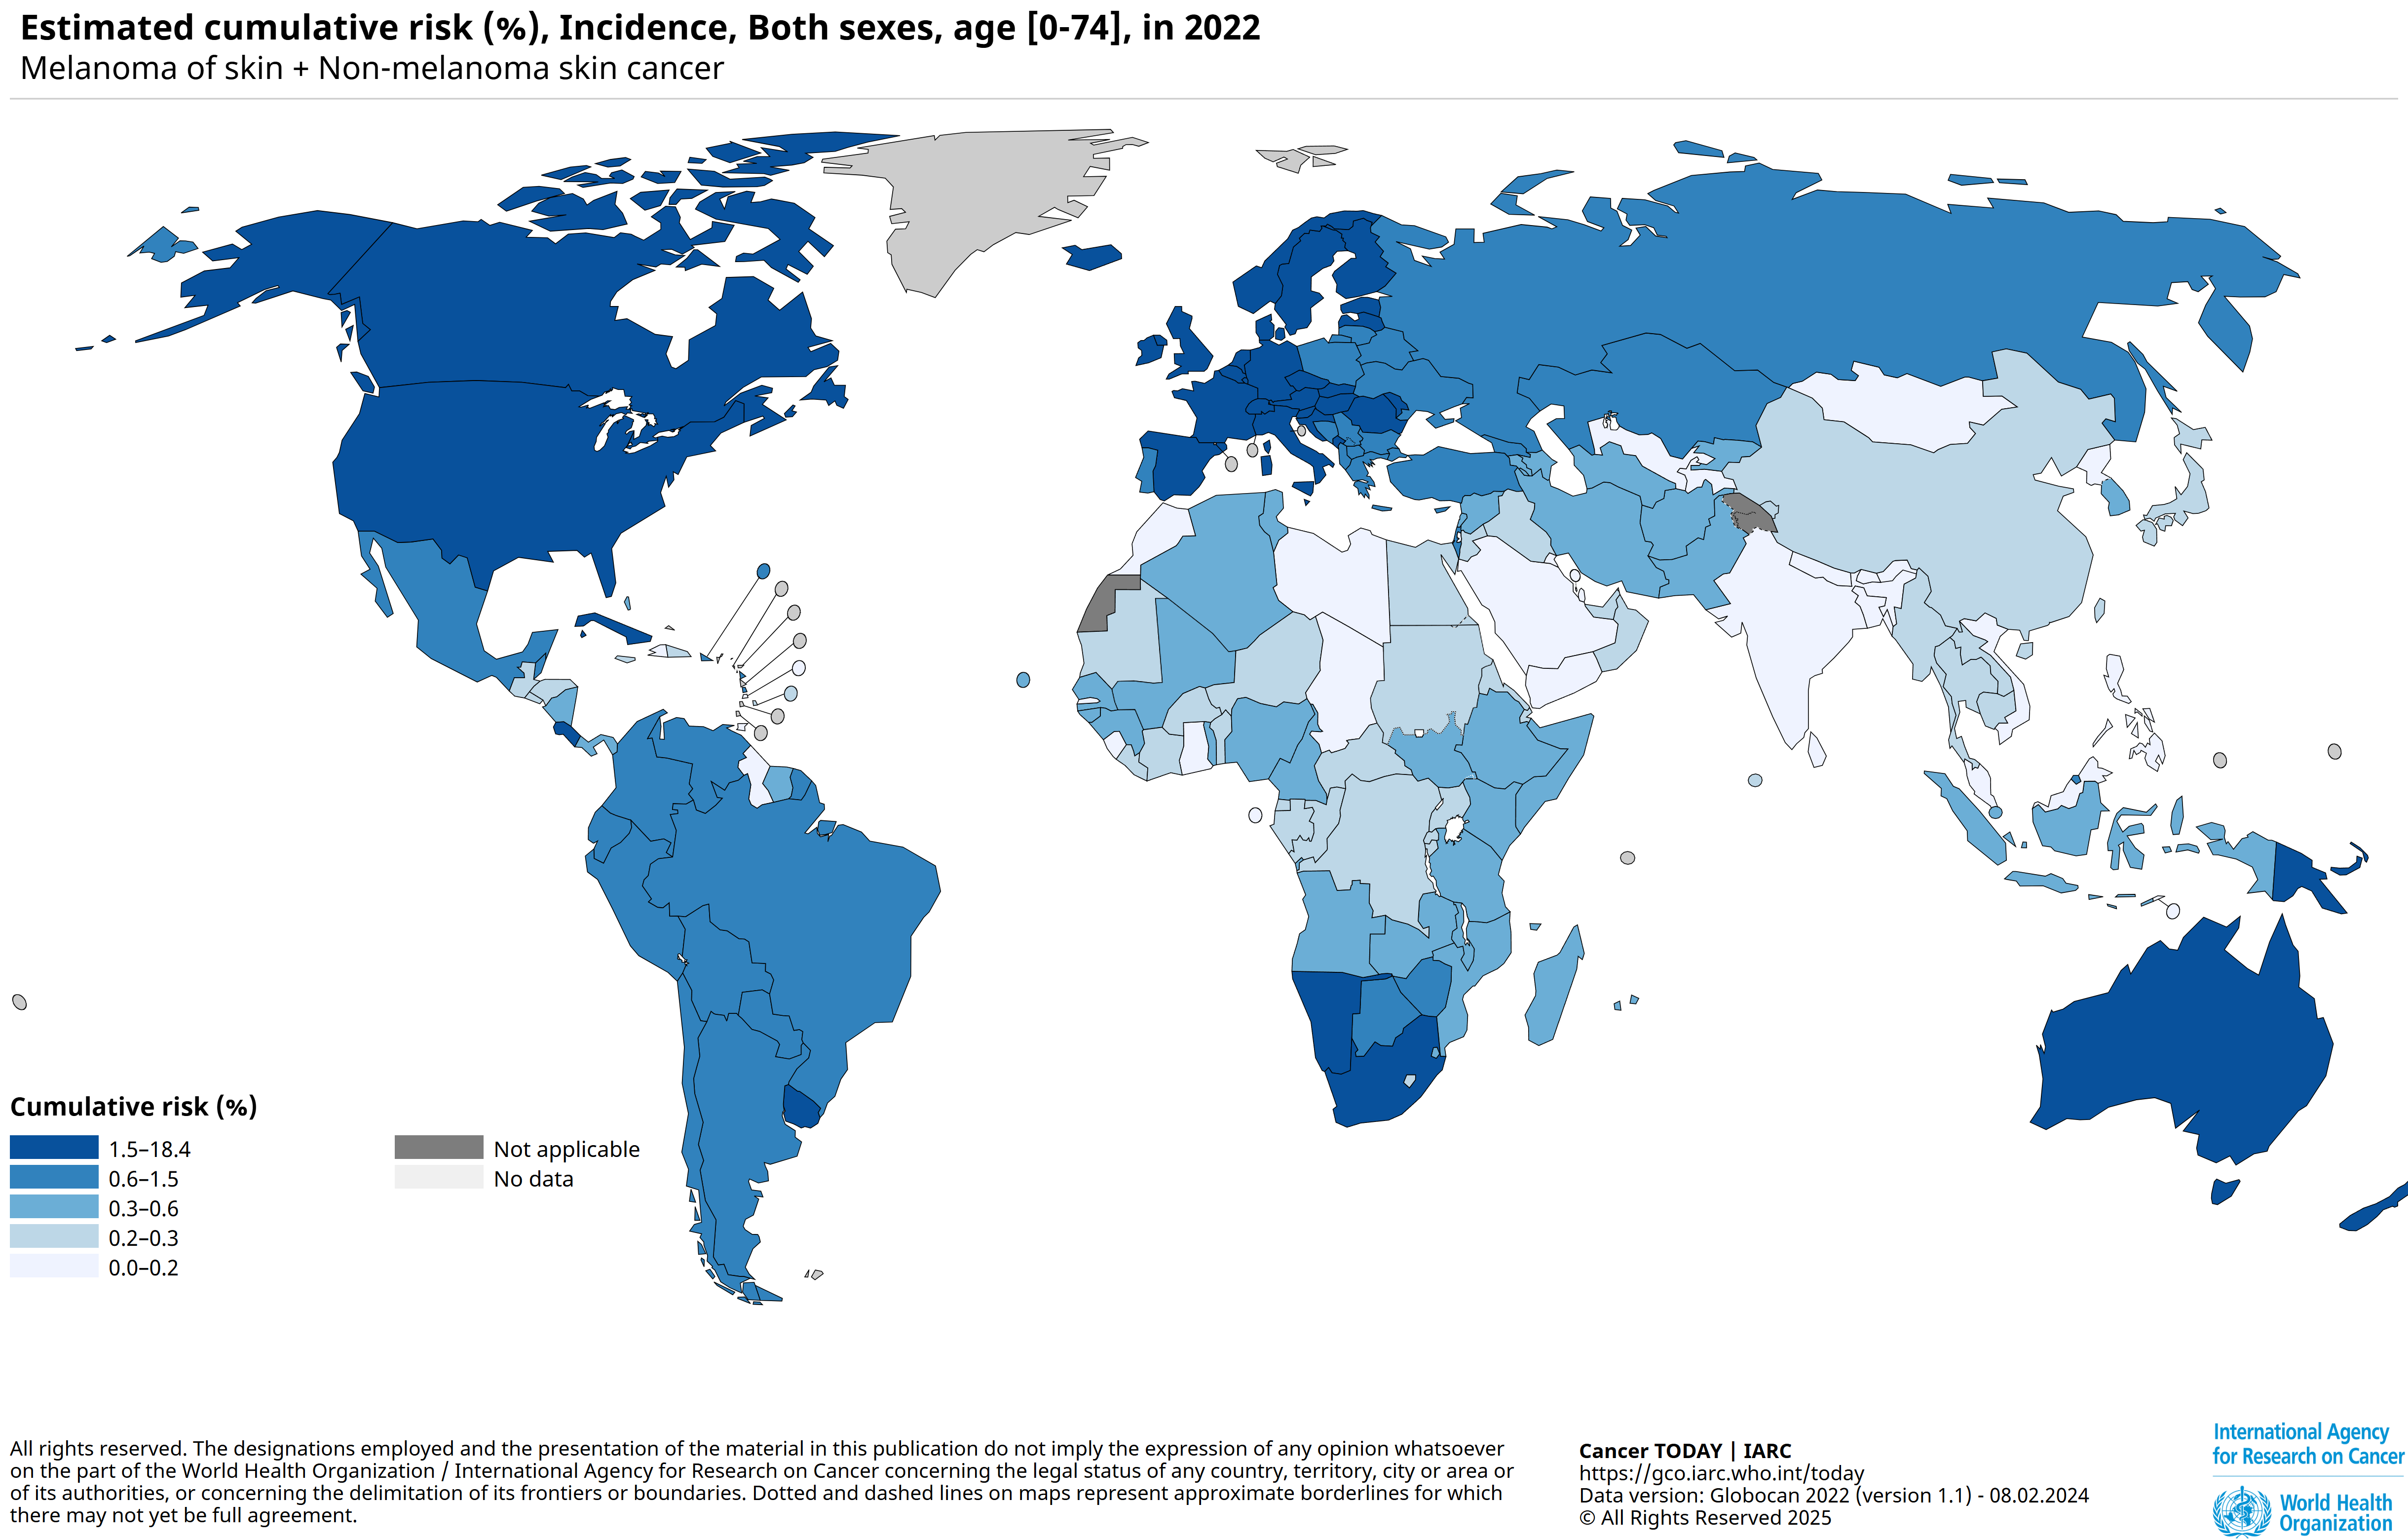
\includegraphics[width=0.95\textwidth]{imagens/Ch2/Sec1.1.png}
	\caption{Risco cumulativo estimado (\%) de incidência de câncer de pele (melanoma e não melanoma), ambos os sexos, entre 0 e 74 anos, em 2022. As áreas em azul-escuro indicam maior risco de desenvolvimento da doença. Fonte: \citeonline{iarc2022globocan}.}
	\label{fig:epidemiologia}
\end{figure}

No Brasil, o câncer de pele representa o tipo mais incidente. O Instituto Nacional de Câncer (INCA) estima que, no triênio 2023–2025, ocorram mais de 220 mil novos casos anuais de câncer de pele não melanoma, correspondendo a aproximadamente 31\% de todos os diagnósticos de câncer no país \cite{inca2023estimativa}. Embora menos frequente, o melanoma é responsável pela maioria das mortes relacionadas ao câncer de pele, devido ao seu alto potencial metastático e rápida progressão em estágios avançados.

A relevância clínica do tema reside na importância do diagnóstico precoce. Estudos epidemiológicos indicam que a taxa de sobrevida em cinco anos para pacientes com melanoma detectado precocemente pode ultrapassar 90\%, enquanto em estágios avançados esse índice pode cair para menos de 20\% \cite{garbe2009melanoma}. Nesse contexto, estratégias de rastreamento e tecnologias de apoio, como sistemas automatizados baseados em inteligência artificial, tornam-se essenciais para ampliar o acesso ao diagnóstico e reduzir a mortalidade em regiões com escassez de especialistas.


\subsection{Características clínicas e dermatoscópicas}

A avaliação clínica inicial das lesões cutâneas suspeitas de melanoma baseia-se amplamente no mnemônico \textit{ABCDE} (\textit{Asymmetry, Border irregularity, Color variegation, Diameter, Evolution}), um método difundido em triagem e educação em saúde. Em termos práticos, lesões assimétricas, com bordas irregulares, variação de cores e diâmetro superior a 6\,mm, ou que apresentem evolução morfológica e cromática recente, devem ser investigadas de forma mais aprofundada \cite{abbasi2004early}. A Figura~\ref{fig:abcd_comparison} ilustra exemplos clínicos de lesões benignas e malignas, evidenciando as diferenças morfológicas e cromáticas associadas a cada condição.

\begin{figure}[H]
	\centering
	\begin{subfigure}[b]{0.45\textwidth}
		\centering
		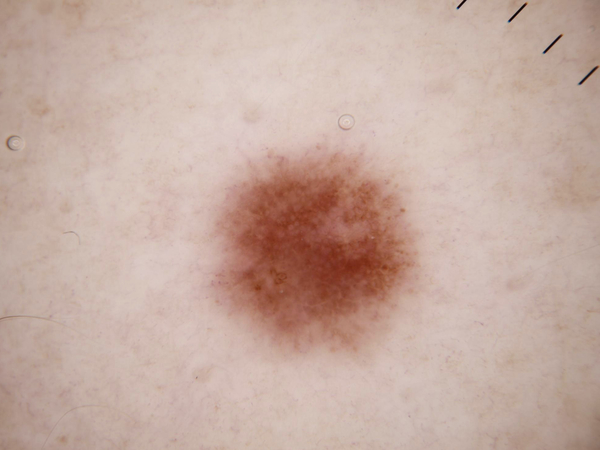
\includegraphics[width=\textwidth]{imagens/Ch2/Sec1.2_Benigna.jpg}
		\caption{Lesão benigna – coloração homogênea e contorno regular.}
		\label{fig:benign_lesion}
	\end{subfigure}
	\hfill
	\begin{subfigure}[b]{0.45\textwidth}
		\centering
		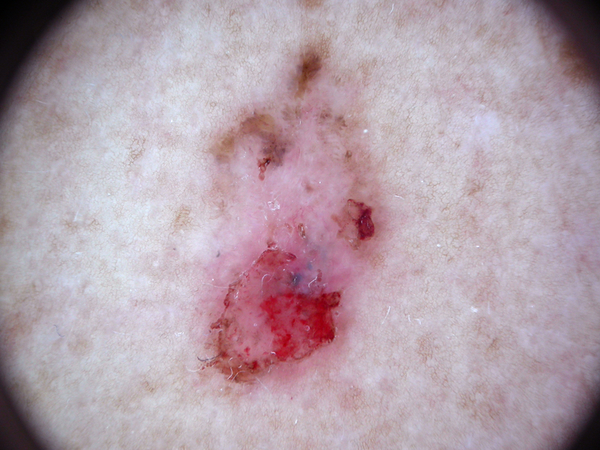
\includegraphics[width=\textwidth]{imagens/Ch2/Sec1.2_Maligna.jpg}
		\caption{Lesão maligna – assimetria, múltiplas cores e bordas irregulares.}
		\label{fig:malignant_lesion}
	\end{subfigure}
	\caption{Comparação visual entre lesões benignas e malignas segundo o método \textit{ABCDE}. A análise clínica considera assimetria, irregularidade de bordas, variação de cor, diâmetro e evolução temporal. Imagens adaptadas do conjunto público ISIC Archive \cite{tschandl2018ham10000}.}
	\label{fig:abcd_comparison}
\end{figure}

Embora simples e de fácil adoção, o \textit{ABCDE} é um instrumento essencialmente clínico-visual, sensível a variações de iluminação, distância focal e resolução da imagem, o que reforça a necessidade de padronização do registro fotográfico, sobretudo em aplicações automatizadas. Em nível submacroscópico, a dermatoscopia adiciona informações estruturais e cromáticas não acessíveis ao exame clínico convencional, aumentando significativamente a acurácia diagnóstica frente à inspeção a olho nu \cite{kittler2002diagnostic}.

Entre os principais algoritmos dermatoscópicos destacam-se: (i) a regra \textit{ABCD da dermatoscopia}, que quantifica Assimetria, Bordas, Cor e Estruturas (\textit{Dermoscopic structures}) mediante pontuação contínua; (ii) o \textit{Seven-Point Checklist} (SPCL), que organiza critérios maiores e menores para indicar probabilidade de melanoma; e (iii) o Método de Menzies, que utiliza dois critérios negativos (padrão simétrico e cor única) e um conjunto de critérios positivos, como véu azul-branco, múltiplos pontos marrons, pseudópodes, \textit{radial streaming}, despigmentação em cicatriz, pontos/glóbulos pretos periféricos e presença de cinco a seis cores \cite{nachbar1994abcd,argenziano2003consensus,argenziano2010sevenpoint,menzies1996frequency}. 

É importante salientar que muitos desses critérios (por exemplo, véu azul-branco, rede pigmentada e pseudópodes) são típicos da dermatoscopia (polarizada ou não) e podem não ser captáveis em fotografias clínicas comuns. Essa distinção é essencial no desenho metodológico: \textit{pipelines} que operam apenas com imagens clínicas devem privilegiar atributos morfológicos globais (assimetria geométrica, irregularidade de contorno, variação global de cor e textura) e medidas derivadas da segmentação (área, razão de eixos, circularidade), reservando a interpretação de estruturas dermatoscópicas para conjuntos de dados adequadamente adquiridos \cite{kittler2002diagnostic,tschandl2018ham10000}. 

De forma convergente, estudos recentes indicam que tanto a análise manual assistida por dermatoscopia quanto modelos computacionais treinados com esse tipo de imagem tendem a superar o desempenho baseado somente em fotografias clínicas, reforçando o ganho de informação desse modo de aquisição \cite{kittler2002diagnostic,haenssle2018man}. No contexto deste trabalho, essa limitação é explicitamente considerada na seleção de características e no desenho dos agentes, de forma a alinhar as expectativas de desempenho às propriedades do dado disponível.


\section{Redes Neurais Artificiais}
\subsection{Fundamentos das RNAs}

\begin{figure}[H]
\centering
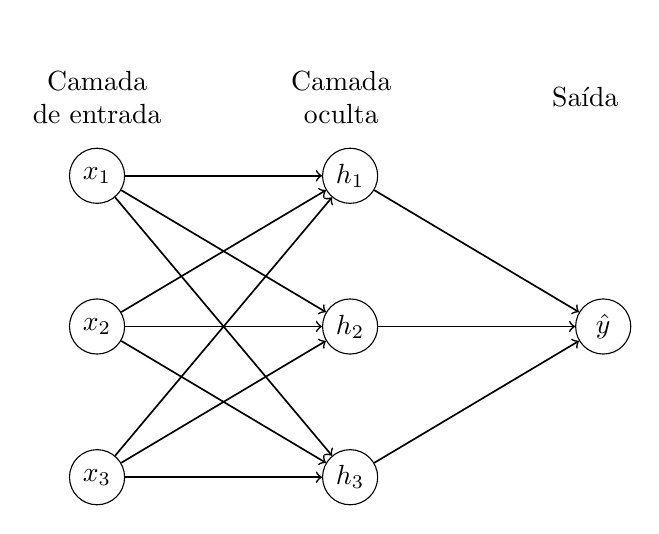
\begin{tikzpicture}[
    node distance=12mm,
    every node/.style={circle, draw, minimum size=7mm, inner sep=0pt}
]
% Input layer
\node (x1) at (0,0) {$x_1$};
\node (x2) [below=of x1] {$x_2$};
\node (x3) [below=of x2] {$x_3$};

% Hidden layer
\node (h1) [right=25mm of x1] {$h_1$};
\node (h2) [below=of h1] {$h_2$};
\node (h3) [below=of h2] {$h_3$};

% Output layer
\node (y1) [right=25mm of h2] {$\hat{y}$};

% Connections: input -> hidden
\foreach \i in {x1,x2,x3}
  \foreach \j in {h1,h2,h3}
    \draw[->, line width=0.6pt] (\i) -- (\j);

% Connections: hidden -> output
\foreach \j in {h1,h2,h3}
  \draw[->, line width=0.6pt] (\j) -- (y1);

% Text boxes (optional)
\node[draw=none, align=center] at (0, 1) {Camada\\ de entrada};
\node[draw=none, align=center] at (3.1, 1) {Camada\\ oculta};
\node[draw=none, align=center] at (6.2, 1) {Saída};

\end{tikzpicture}
\caption{Esquema autoral de uma rede neural feedforward (MLP) com uma camada oculta. A figura ilustra a conexão total entre camadas e a noção de transformação não linear.}
\label{fig:mlp_schematic}
\end{figure}


As Redes Neurais Artificiais (RNAs) constituem a base teórica do aprendizado profundo e são inspiradas em mecanismos biológicos do cérebro humano. Seu princípio fundamental consiste em unidades computacionais denominadas neurônios artificiais, organizadas em camadas, que processam sinais de entrada, aplicam funções de ativação e produzem saídas ajustáveis por meio de um processo de treinamento. Esse treinamento é realizado, em geral, pelo algoritmo de retropropagação do erro, que ajusta os pesos das conexões neuronais de forma iterativa até minimizar a função de perda \cite{rumelhart1986learning}.

O avanço das RNAs está intrinsecamente ligado à disponibilidade de dados em larga escala e ao aumento do poder computacional. A partir da década de 2010, o campo de aprendizado profundo (\textit{deep learning}) emergiu como uma abordagem dominante, trazendo inovações arquiteturais que impulsionaram a performance em diversas tarefas, como reconhecimento de imagens, processamento de linguagem natural e diagnóstico médico assistido por computador \cite{lecun2015deep, schmidhuber2015deep}. No contexto da saúde, as RNAs permitem identificar padrões complexos em imagens clínicas que seriam de difícil percepção por métodos convencionais de análise estatística, aumentando a acurácia e reduzindo a variabilidade intra e interobservador.

A relevância das RNAs no diagnóstico médico decorre da sua capacidade de generalização a partir de exemplos rotulados. Ao aprender a mapear representações de alto nível a partir de dados brutos, esses modelos conseguem captar características discriminativas úteis para tarefas como classificação de lesões cutâneas, diferenciação entre imagens normais e patológicas e detecção precoce de anomalias \cite{goodfellow2016deep}. No entanto, o desempenho das RNAs depende fortemente da qualidade dos dados disponíveis, sendo suscetíveis a sobreajuste (\textit{overfitting}) em bases pequenas ou desbalanceadas, o que torna essencial o uso de técnicas complementares, como regularização e aumento de dados (\textit{data augmentation}).


\subsection{Redes Neurais Convolucionais (CNNs)}

As Redes Neurais Convolucionais (CNNs) representam uma evolução das Redes Neurais Artificiais tradicionais, sendo projetadas especificamente para o processamento de dados com estrutura espacial, como imagens bidimensionais. Sua principal inovação reside na aplicação de filtros convolucionais que percorrem a imagem extraindo características locais,  como bordas, texturas e formas,  em diferentes níveis de abstração. Essa estratégia permite reduzir a dimensionalidade dos dados sem perda significativa de informação relevante e explorar de maneira eficiente as correlações espaciais entre pixels \cite{lecun1998gradient}.

A Figura~\ref{fig:lenet_architecture} apresenta a arquitetura clássica da rede LeNet-5, uma das primeiras CNNs bem-sucedidas desenvolvidas por LeCun e colaboradores. O modelo é composto por uma sequência de camadas convolucionais, funções de ativação não lineares, camadas de \textit{subsampling} (ou \textit{pooling}) para redução espacial e camadas totalmente conectadas responsáveis pela classificação final. Essa hierarquia permite que o modelo construa progressivamente representações mais complexas: camadas iniciais detectam padrões simples (como linhas e bordas), enquanto camadas mais profundas aprendem estruturas de maior abstração, como formas e texturas características de lesões cutâneas \cite{krizhevsky2012imagenet}.

\begin{figure}[H]
	\centering
	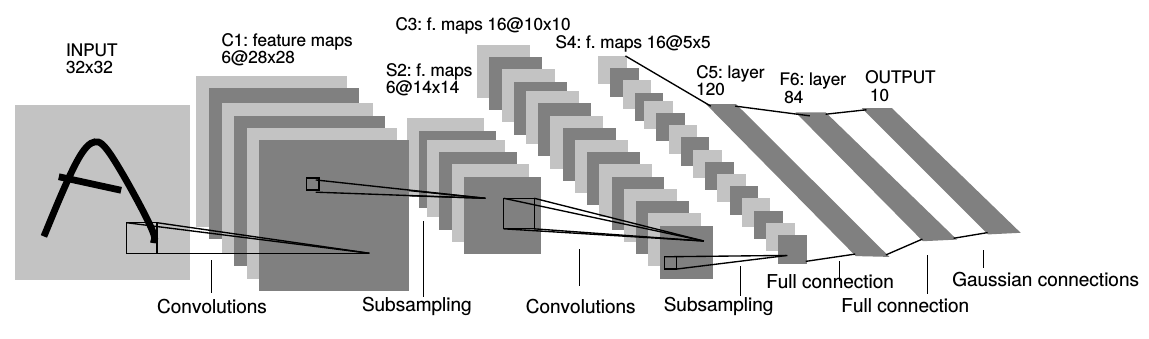
\includegraphics[width=0.95\textwidth]{imagens/Ch2/Sec2.2.png}
	\caption{Arquitetura clássica da rede convolucional LeNet-5, proposta por \citeonline{lecun1998gradient}. A rede é composta por camadas convolucionais intercaladas com operações de \textit{subsampling}, seguidas por camadas totalmente conectadas responsáveis pela classificação. Essa estrutura serviu de base para o desenvolvimento das CNNs modernas.}
	\label{fig:lenet_architecture}
\end{figure}

No campo médico, as CNNs têm demonstrado desempenho superior em tarefas de diagnóstico por imagem, incluindo radiologia, patologia digital e dermatologia. Trabalhos pioneiros mostraram que CNNs podem alcançar resultados comparáveis aos de especialistas humanos na classificação de lesões cutâneas malignas e benignas a partir de imagens dermatoscópicas \cite{esteva2017dermatologist,haenssle2018man}. Essa capacidade decorre da habilidade dessas redes em identificar padrões sutis frequentemente imperceptíveis ao olho humano, fornecendo suporte relevante para decisões clínicas.

Entretanto, a aplicação de CNNs em contextos médicos apresenta desafios particulares. Entre eles estão a necessidade de grandes volumes de dados anotados com precisão, o risco de sobreajuste (\textit{overfitting}) em conjuntos reduzidos e a limitada interpretabilidade dos modelos, frequentemente descritos como “caixas-pretas” \cite{holzinger2017we}. Para mitigar essas limitações, pesquisas recentes têm explorado o uso de arquiteturas híbridas e técnicas de explicabilidade, como \textit{Grad-CAM}, que permitem visualizar as regiões da imagem mais relevantes para a decisão do modelo, aumentando a transparência e a confiança clínica.


\subsection{Redes de Atenção e Transformers}

O mecanismo de atenção foi introduzido como uma solução para superar as limitações dos modelos sequenciais tradicionais, como as redes neurais recorrentes (RNNs), que apresentavam dificuldades em capturar dependências de longo alcance em tarefas de processamento de linguagem natural. A atenção permite que o modelo atribua pesos diferenciados a partes distintas da entrada, concentrando-se seletivamente nas informações mais relevantes para a tarefa em execução \cite{bahdanau2014neural}. 

Esse conceito foi expandido pelo \textit{Transformer}, proposto por \citeonline{vaswani2017attention}, que substituiu completamente a recorrência pelo uso de múltiplos cabeçalhos de atenção (\textit{multi-head attention}) e mecanismos de normalização, tornando-se o paradigma dominante em modelos de linguagem. A Figura~\ref{fig:transformer_architecture} ilustra a arquitetura básica do Transformer, composta por blocos de \textit{encoder} e \textit{decoder}, nos quais o mecanismo de atenção é aplicado em paralelo a camadas de normalização e redes alimentadas adiante (\textit{feed-forward}).

\begin{figure}[H]
	\centering
	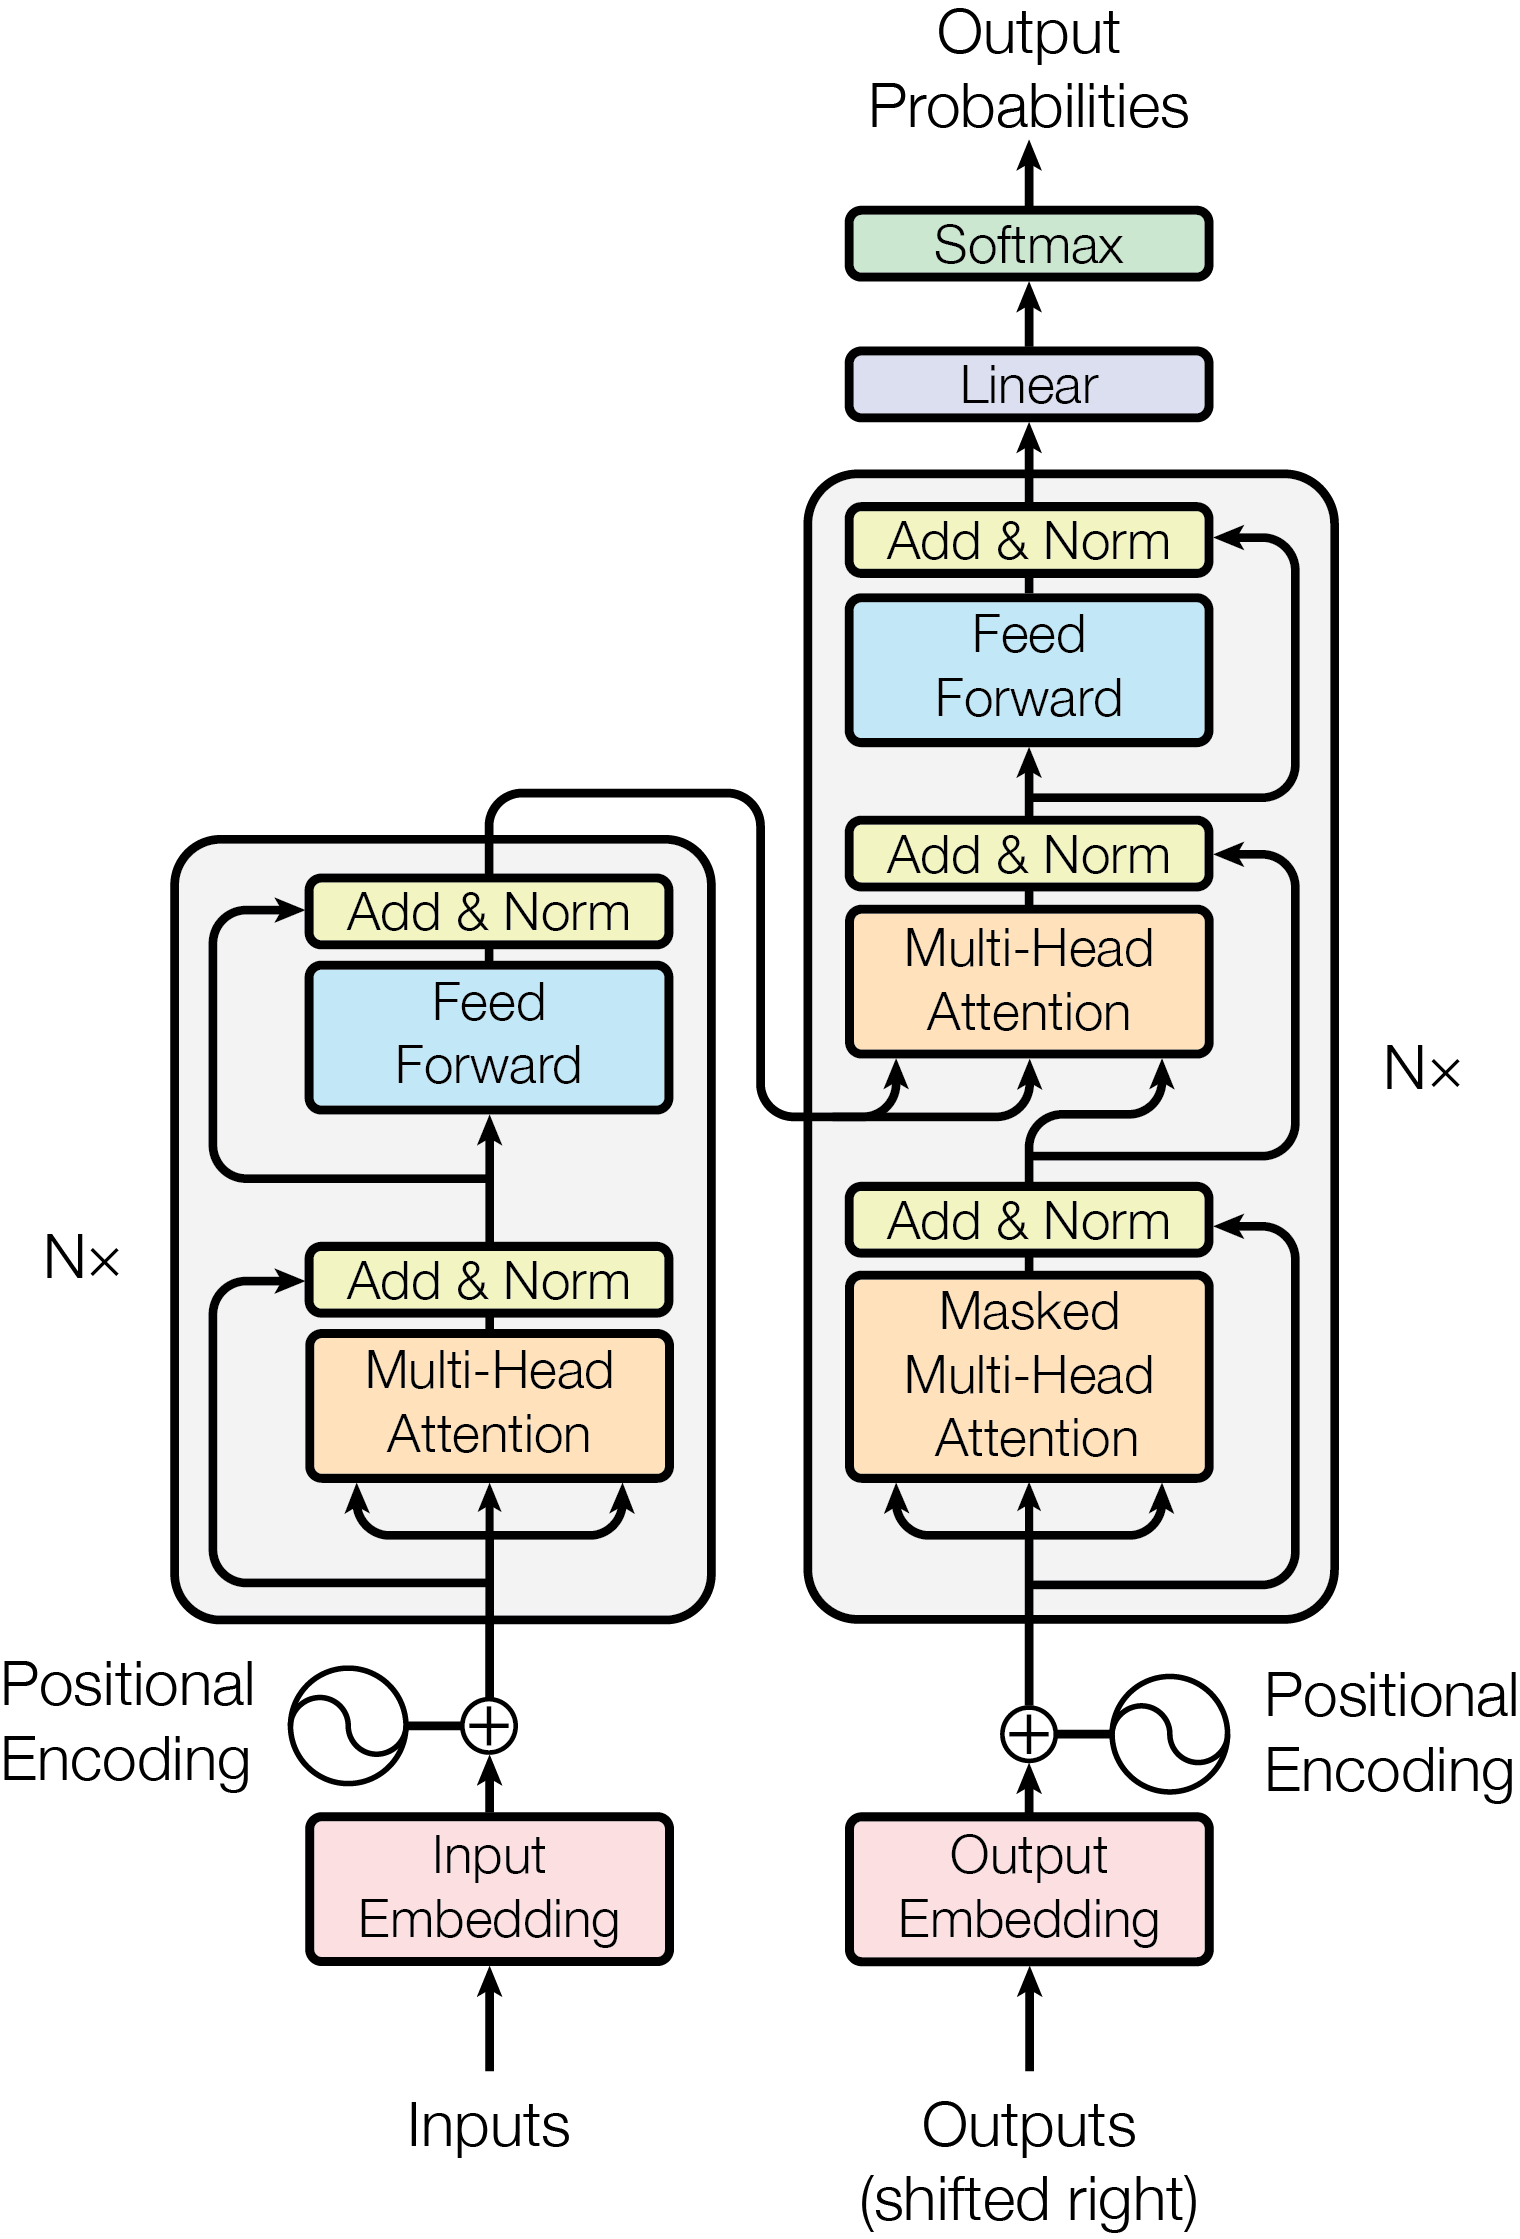
\includegraphics[width=0.85\textwidth]{imagens/Ch2/Sec2.4.png}
	\caption{Arquitetura do modelo Transformer proposto por \citeonline{vaswani2017attention}, composta por blocos de \textit{encoder} e \textit{decoder} conectados por mecanismos de atenção multi-cabeças. Essa estrutura permitiu substituir totalmente a recorrência e impulsionou o desenvolvimento de modelos de linguagem e visão em larga escala.}
	\label{fig:transformer_architecture}
\end{figure}

Nos últimos anos, a arquitetura Transformer ultrapassou o domínio textual e passou a ser aplicada ao processamento de imagens, originando os \textit{Vision Transformers} (ViT). Nessa abordagem, a imagem é dividida em pequenos blocos (\textit{patches}) que são tratados como sequências análogas a palavras em um texto, permitindo ao modelo aprender representações globais da cena \cite{dosovitskiy2021an}. Essa capacidade de modelar relações de longo alcance entre regiões da imagem contrasta com a natureza local das convoluções em CNNs, tornando os Transformers especialmente eficazes em capturar padrões estruturais complexos e contextuais.

No campo da saúde, os Transformers têm se mostrado competitivos ou mesmo superiores às CNNs em diversas tarefas, incluindo classificação de radiografias, análise histopatológica e segmentação de lesões cutâneas. Arquiteturas híbridas, como a TransUNet, combinam convoluções nas etapas iniciais para extrair detalhes locais e módulos de atenção para capturar dependências globais, atingindo resultados de ponta em segmentação médica \cite{chen2021transunet}. Em dermatologia, estudos recentes demonstram que modelos baseados em Transformers podem superar CNNs tradicionais na classificação de imagens de melanoma e outras lesões pigmentadas, especialmente quando aliados a abordagens multimodais que integram dados clínicos e visuais \cite{liu2021swin,raghu2021vision}.

Apesar dos avanços, desafios persistem quanto ao alto custo computacional do treinamento de Transformers e à necessidade de grandes volumes de dados anotados para evitar sobreajuste. Em contextos médicos, nos quais os conjuntos de dados são frequentemente limitados, estratégias como \textit{transfer learning}, autoaprendizado e pré-treinamento multimodal têm se mostrado essenciais para viabilizar sua aplicação prática \cite{khan2022transformers}.


\section{Segmentação de Imagens}
\label{sec:segmentacao}

A segmentação de imagens médicas representa uma das etapas mais fundamentais do processamento computacional em saúde, pois possibilita a identificação precisa de estruturas anatômicas e patológicas, permitindo a quantificação de áreas de interesse e a extração de descritores morfológicos relevantes. Essa técnica é empregada de forma transversal em diversas modalidades diagnósticas, desde exames de imagem de alta resolução até registros clínicos convencionais. A Figura~\ref{fig:segmentacao_medica_exemplos} ilustra esse caráter generalista, apresentando exemplos de segmentação em ressonância magnética cerebral, dermatoscopia e tomografia computadorizada pulmonar.

As três modalidades representadas não têm o objetivo de comparação direta, mas de evidenciar a natureza universal do processo de segmentação,  um mesmo princípio algorítmico capaz de isolar regiões de interesse sob diferentes perspectivas e condições de aquisição. Em ressonância magnética, a segmentação permite delimitar tumores cerebrais e quantificar volumes afetados, contribuindo para protocolos de neurocirurgia e acompanhamento terapêutico \cite{minaee2021image}. Em dermatoscopia, a técnica destaca as fronteiras entre a lesão pigmentada e a pele saudável, fornecendo uma base morfológica para classificadores que diferenciam lesões benignas e malignas \cite{tschandl2018ham10000}. Já em tomografia computadorizada, é aplicada na detecção e mensuração de nódulos pulmonares, oferecendo suporte ao rastreamento precoce de neoplasias \cite{shen2017deep}.

A escolha dessas representações se justifica pela coerência conceitual entre os domínios: embora as propriedades ópticas, os artefatos e os parâmetros físicos variem entre modalidades, o núcleo computacional da segmentação,  baseado em extração hierárquica de características espaciais e reconstrução morfológica,  permanece o mesmo. Essa convergência técnica reforça a plausibilidade de estender arquiteturas já consolidadas, como a U-Net \cite{ronneberger2015unet}, ao domínio da dermatologia. No contexto desta pesquisa, a segmentação é concebida não apenas como um pré-processamento visual, mas como a etapa estruturante que possibilita a análise textual posterior por modelos de linguagem natural e agentes colaborativos, sustentando assim a integração entre visão computacional e raciocínio clínico automatizado.

\begin{figure}[H]
	\centering
	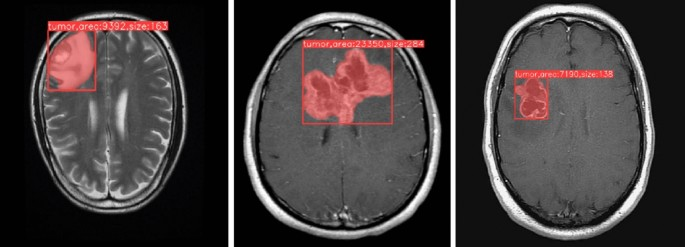
\includegraphics[width=0.32\textwidth]{imagens/Ch2/Sec2.3.Intro1.jpg}
	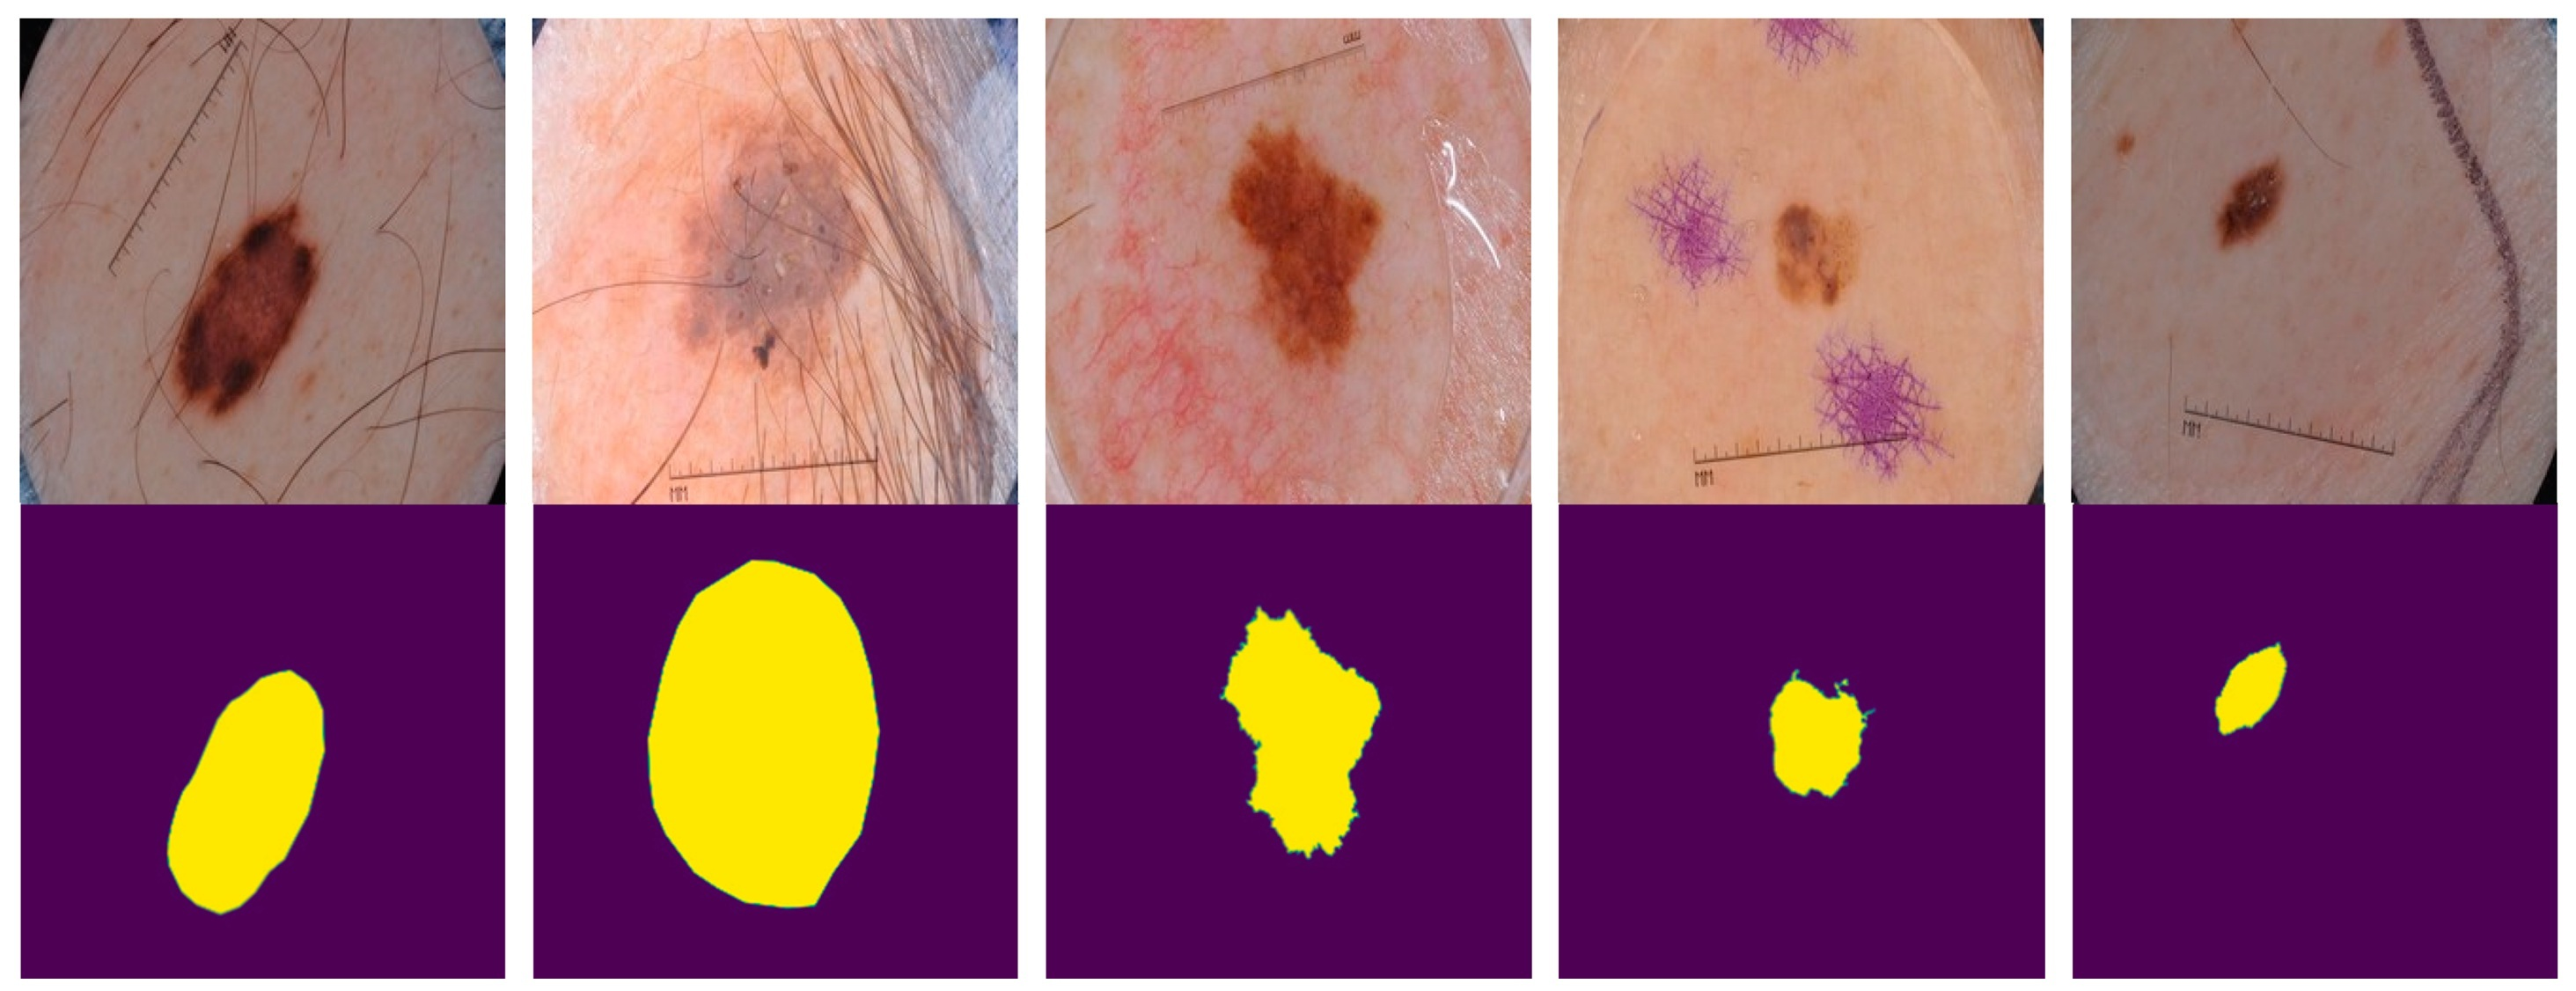
\includegraphics[width=0.32\textwidth]{imagens/Ch2/Sec2.3.Intro2.jpg}
	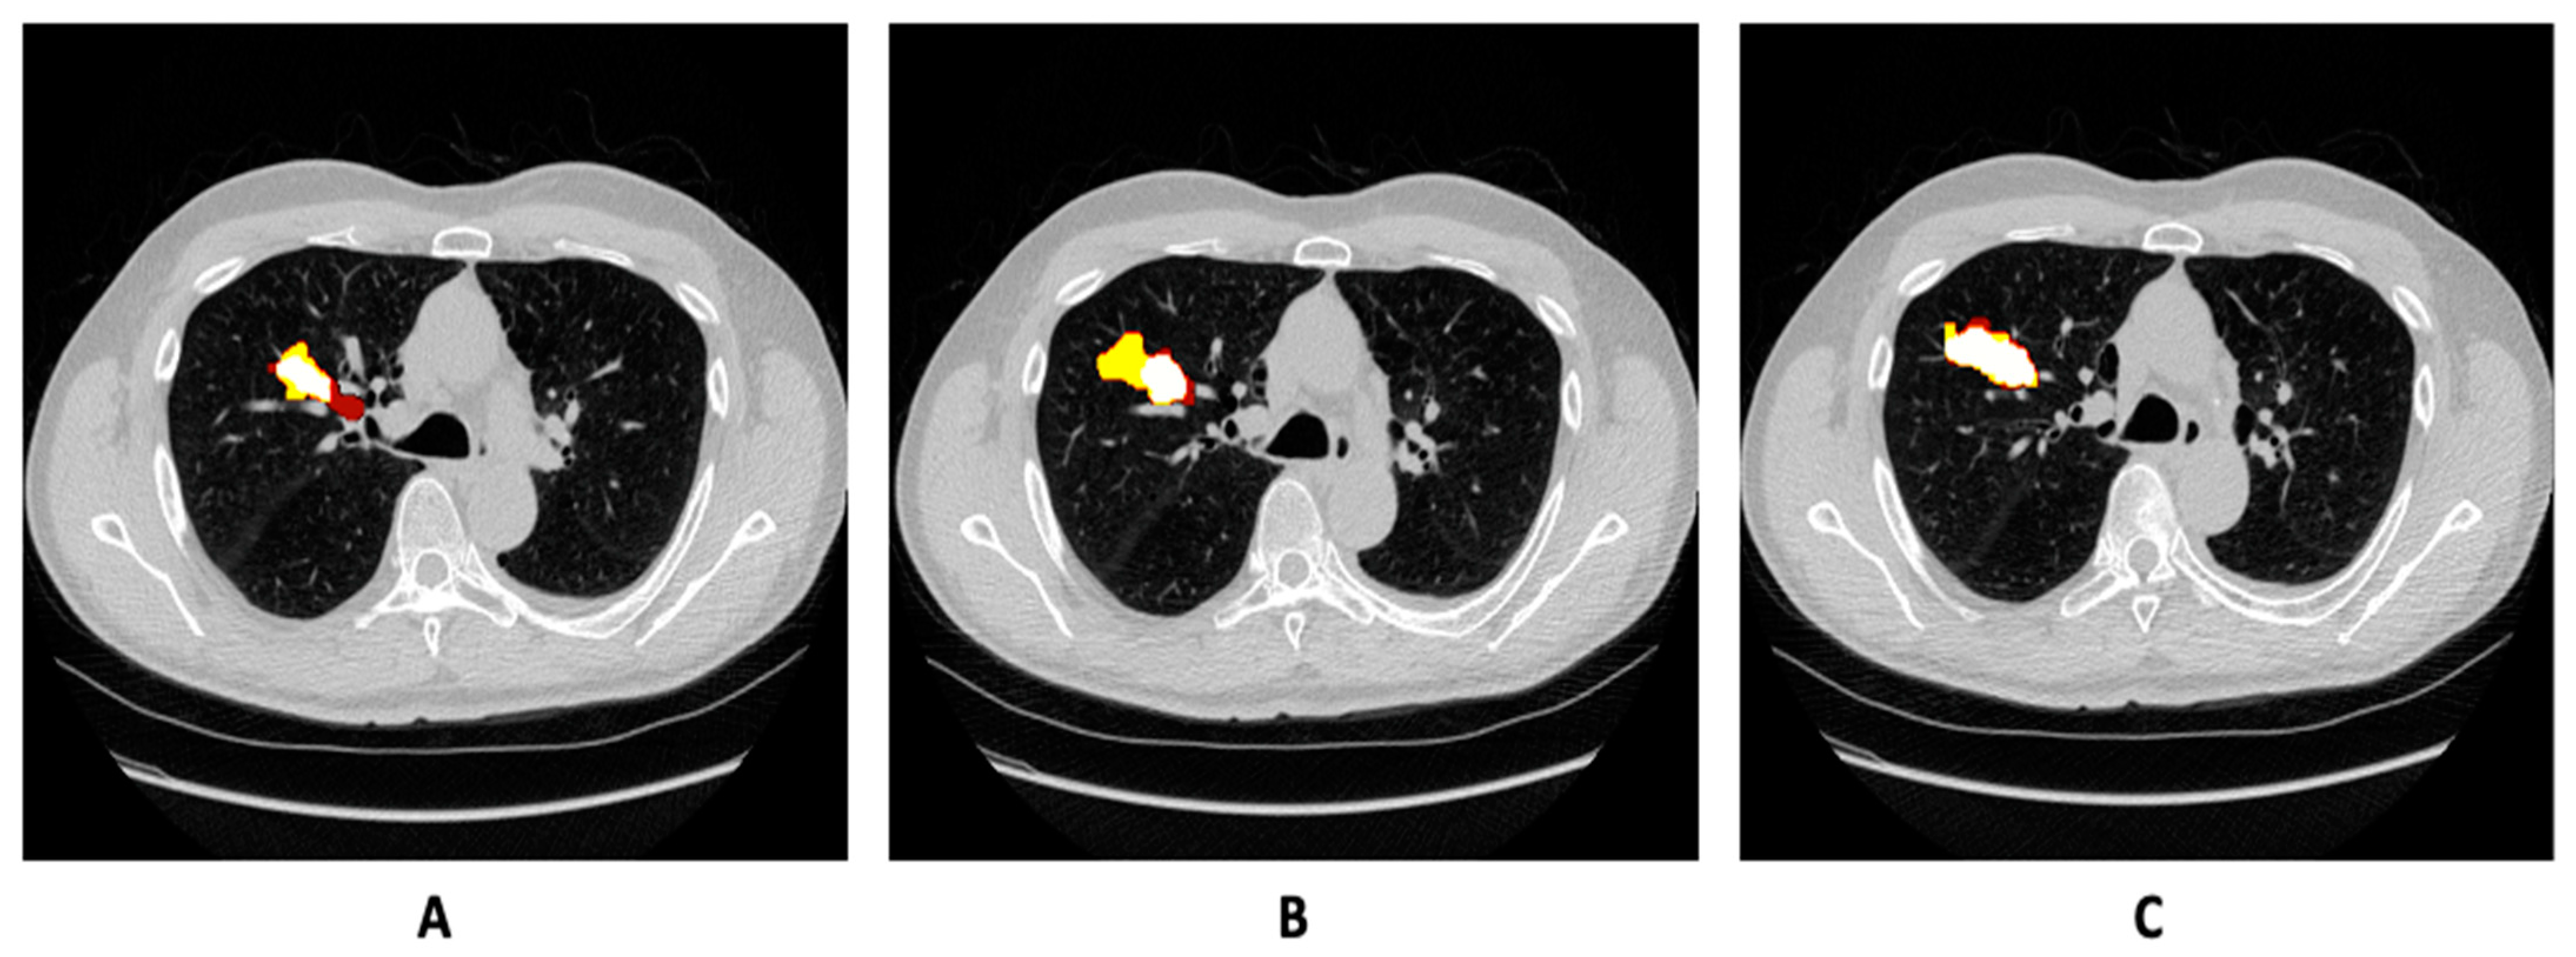
\includegraphics[width=0.32\textwidth]{imagens/Ch2/Sec2.3.Intro3.jpg}
	\caption{
		Exemplos de aplicação da segmentação em diferentes modalidades médicas: 
		(A) delineamento de tumor cerebral em ressonância magnética \cite{minaee2021image}, 
		(B) isolamento de lesão cutânea pigmentada em dermatoscopia \cite{tschandl2018ham10000}, e 
		(C) segmentação de nódulos pulmonares em tomografia computadorizada \cite{shen2017deep}.
		As imagens foram reproduzidas e adaptadas de seus respectivos estudos para fins ilustrativos e acadêmicos.}
	\label{fig:segmentacao_medica_exemplos}
\end{figure}

\subsection{Tipos de Segmentação de Imagens Médicas}

A segmentação de imagens médicas constitui uma das tarefas mais fundamentais em visão computacional aplicada à saúde, permitindo a delimitação precisa de regiões anatômicas ou patológicas de interesse. Diferentes abordagens de segmentação variam quanto ao nível de granularidade e ao tipo de inferência produzida, influenciando diretamente a interpretabilidade e a aplicabilidade clínica do resultado \cite{reinke2021commonlimitations}.

A Figura~\ref{fig:segmentacao_tipos} ilustra, de forma esquemática, os quatro principais paradigmas de predição em visão computacional médica:  
(A) \textbf{classificação de imagem}, na qual a decisão é global e a imagem é associada a um único rótulo;  
(B) \textbf{segmentação semântica}, que rotula cada pixel de acordo com sua classe, permitindo a identificação contínua de regiões homogêneas;  
(C) \textbf{detecção de objetos}, que reconhece e localiza instâncias individuais por meio de \textit{bounding boxes}; e  
(D) \textbf{segmentação por instância}, que combina as abordagens anteriores, distinguindo múltiplos objetos da mesma classe \cite{reinke2021commonlimitations}.

No contexto dermatológico, a \textbf{segmentação semântica} é a mais apropriada, pois as lesões cutâneas tendem a compor uma única estrutura contínua. Nesse caso, o foco analítico recai sobre a geometria da lesão,  área, borda, assimetria e variação de cor,  e não sobre a distinção entre instâncias múltiplas. Essa característica torna o problema mais alinhado a uma formulação pixel a pixel, em que a precisão dos limites é mais relevante do que a diferenciação entre objetos. 

Além disso, o uso da segmentação semântica apresenta vantagens computacionais e metodológicas para integração com sistemas baseados em linguagem natural. Ao delimitar a área de interesse de forma consistente e explicável, o modelo gera uma entrada visual estruturada que pode ser convertida em descrições clínicas compreensíveis por modelos de linguagem (LLMs). Assim, o equilíbrio entre granularidade e interpretabilidade faz da segmentação semântica uma escolha técnica e clinicamente fundamentada para o escopo desta pesquisa.

\begin{figure}[H]
	\centering
	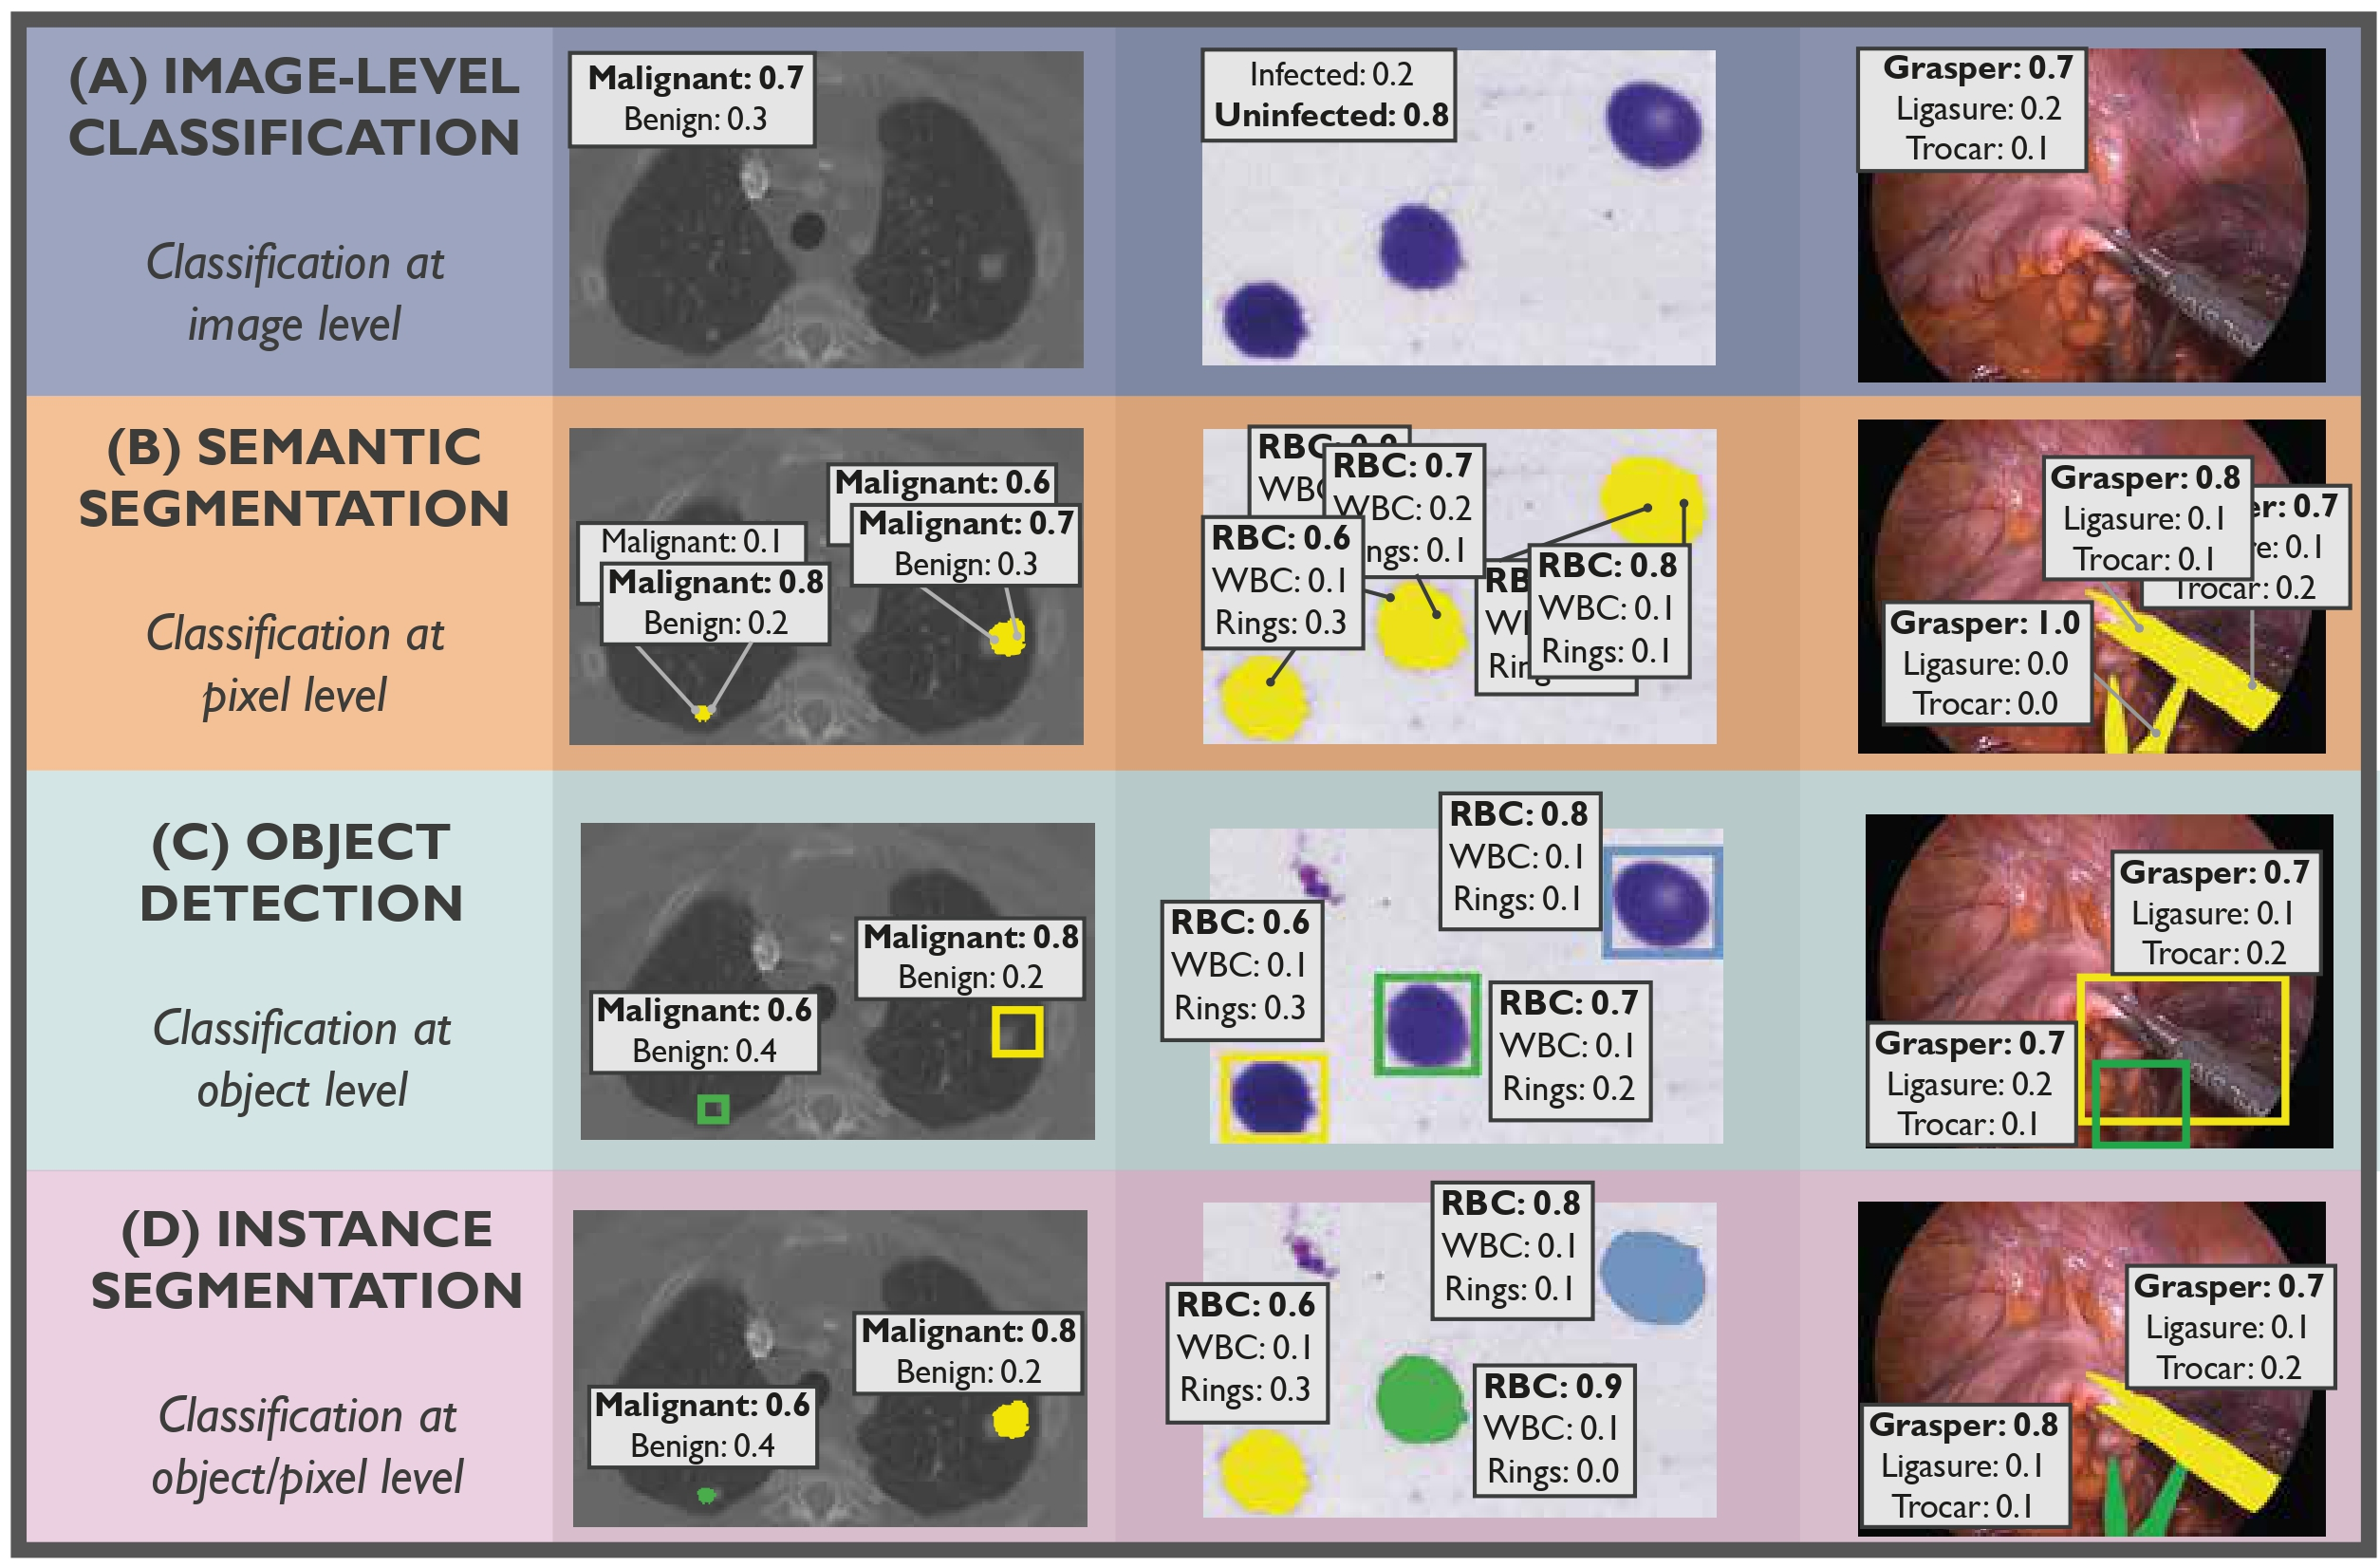
\includegraphics[width=\textwidth]{imagens/Ch2/Section2.3.2.jpg}
	\caption{
		Comparação entre níveis de granularidade em tarefas de visão computacional aplicadas à medicina:
		(A) classificação de imagem,  decisão global por rótulo;
		(B) segmentação semântica,  classificação por pixel;
		(C) detecção de objetos,  reconhecimento e localização de instâncias por caixas delimitadoras; 
		(D) segmentação por instância,  diferenciação individual de múltiplos objetos de mesma classe.
		Adaptado de \citeonline{reinke2021commonlimitations}.}
	\label{fig:segmentacao_tipos}
\end{figure}


\subsection{Arquiteturas baseadas em U-Net}

Desde sua introdução em 2015, a U-Net tornou-se a arquitetura de referência para segmentação de imagens médicas, oferecendo uma combinação eficiente entre simplicidade estrutural e alta capacidade de generalização \cite{ronneberger2015unet}. Sua estrutura em formato de “U”, composta por um caminho de codificação (\textit{encoder}) e outro de decodificação (\textit{decoder}) conectados por \textit{skip connections}, permite extrair características em múltiplas escalas e recuperar informações espaciais perdidas durante o processo de compressão, como ilustrado na Figura~\ref{fig:unet_original}. Essa arquitetura mostrou-se particularmente eficaz em contextos de dados limitados e altamente desbalanceados, como na segmentação de tecidos biológicos, e é apresentada aqui como referência canônica que fundamenta tanto o conceito de \textit{ground truth} de segmentação adotado nesta pesquisa quanto as direções de trabalho futuro.

\begin{figure}[H]
	\centering
	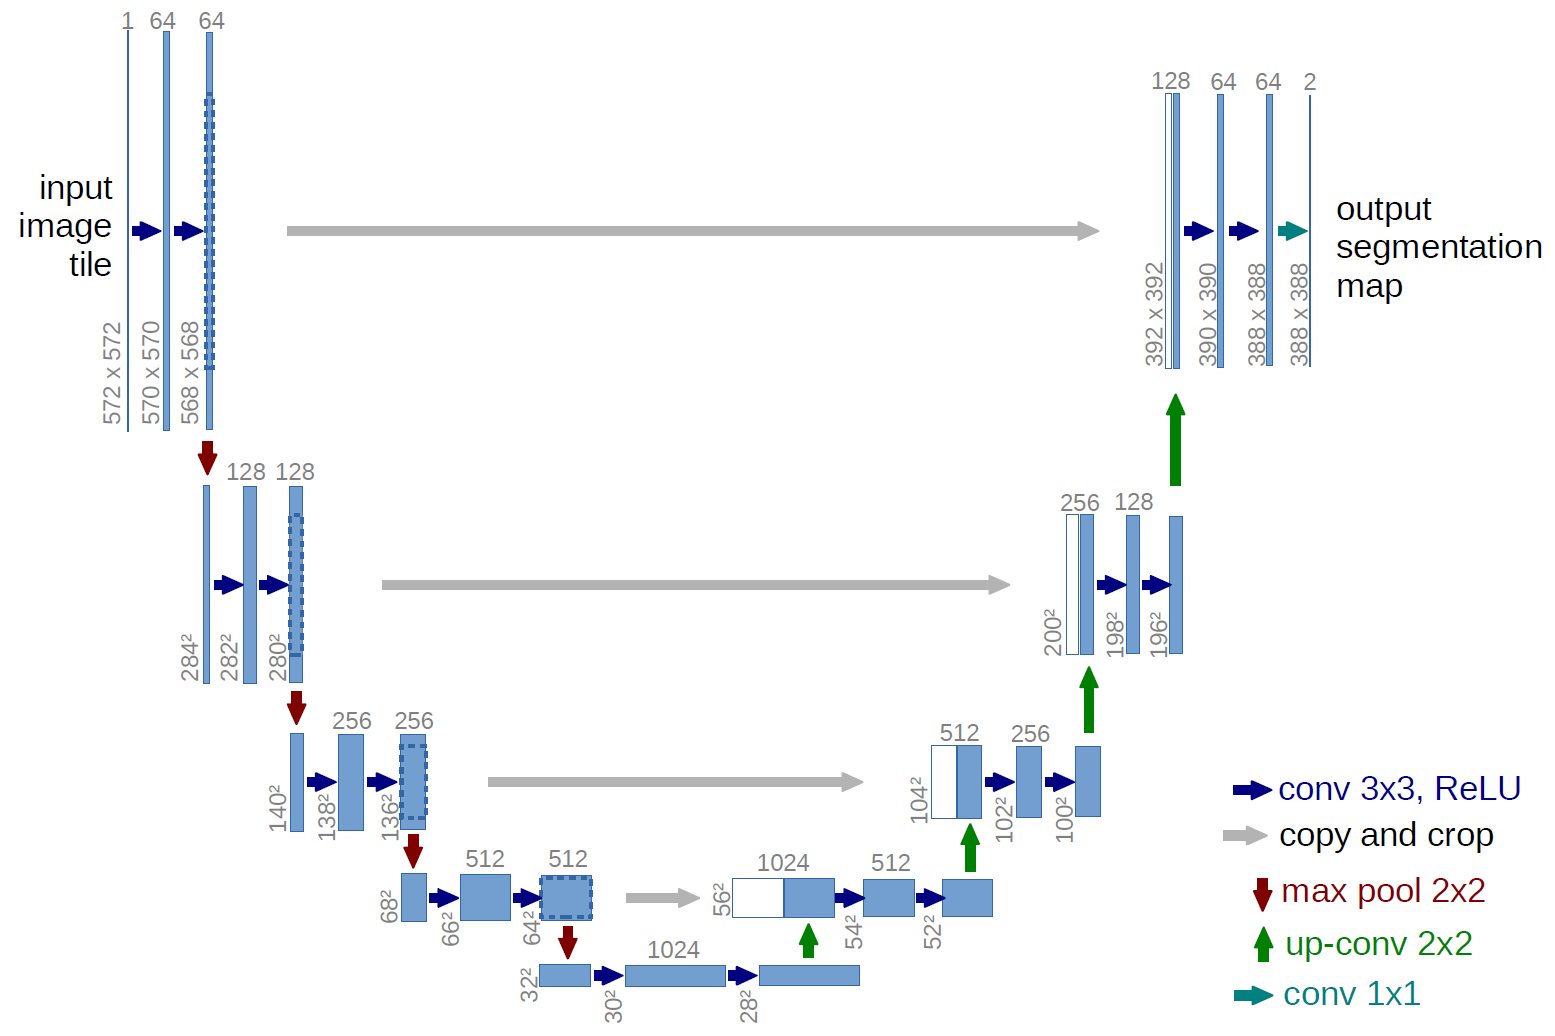
\includegraphics[width=0.9\textwidth]{imagens/Ch2/Sec2.3.png}
	\caption{
		Arquitetura da U-Net clássica \cite{ronneberger2015unet}, composta por um caminho de contração (\textit{encoder}) e um de expansão (\textit{decoder}) conectados por \textit{skip connections}. Essa estrutura permite capturar e reconstruir informações espaciais multiescalares, tornando-a referência em segmentação biomédica.
	}
	\label{fig:unet_original}
\end{figure}

A partir da U-Net clássica, a literatura biomédica desenvolveu variantes que aprimoram aspectos específicos do fluxo de informação. A R2U-Net \cite{alom2018r2unet} incorpora blocos residuais com convoluções recursivas, melhorando a estabilidade de gradiente e a precisão em bordas finas. A Attention U-Net \cite{oktay2018attentionunet} adiciona módulos de atenção espacial nas \textit{skip connections}, permitindo que o modelo suprima automaticamente regiões de fundo e concentre o processamento na lesão, vantagem especialmente relevante em dermatoscopia, onde a lesão ocupa uma fração pequena da cena. A Attention R2U-Net \cite{alom2019attentionr2unet} combina as duas abordagens anteriores, integrando convoluções recursivas e atenção espacial em uma única arquitetura de maior estabilidade e seletividade.

Em síntese, as variantes da U-Net representam uma progressão natural de refinamentos estruturais, que buscam equilibrar desempenho, interpretabilidade e custo computacional. No contexto da presente pesquisa, essas arquiteturas são apresentadas como referencial teórico consolidado para segmentação dermoscópica. A decisão metodológica de adotar as máscaras de referência (\textit{ground truth}) do conjunto PH2 em lugar de segmentações automáticas não invalida sua relevância: ao eliminar a variabilidade introduzida por erros de segmentação, é possível atribuir as diferenças de desempenho exclusivamente à capacidade de raciocínio das LLMs. A integração de um módulo de segmentação automático ao \textit{pipeline} constitui uma direção natural para trabalhos futuros.



\section{Modelos de Linguagem de Larga Escala (LLMs)}

\subsection{Fundamentos}

Os Modelos de Linguagem de Larga Escala (LLMs, do inglês \textit{Large Language Models}) são arquiteturas de aprendizado profundo, em geral baseadas em Transformers, treinadas sobre grandes volumes de dados textuais. Eles possuem bilhões de parâmetros e aprendem representações semânticas que permitem realizar tarefas de compreensão, geração e raciocínio textual \cite{devlin2019bert,brown2020language}. Diferentemente de abordagens anteriores em processamento de linguagem natural (PLN), que eram altamente dependentes de recursos linguísticos manuais, os LLMs capturam padrões complexos diretamente a partir de dados em larga escala, tornando-se modelos de propósito geral capazes de adaptação a múltiplos domínios.

Esses modelos demonstraram desempenho acima do esperado em tarefas de múltipla escolha, resolução de problemas, geração de explicações e sumarização. Sua principal inovação reside na capacidade de generalizar conhecimento aprendido em contextos amplos e aplicá-lo em domínios específicos, frequentemente com pouco ou nenhum ajuste adicional (\textit{zero-shot} e \textit{few-shot learning}) \cite{openai2023gpt4}. No campo da saúde, essa característica é particularmente relevante, visto que permite adaptar o modelo a tarefas médicas sem a necessidade de treinamento extenso em bases clínicas.

\subsection{LLMs com capacidade multimodal}

Uma evolução dos LLMs é a incorporação de entradas multimodais, como imagens e texto. Modelos multimodais, como GPT-5.4-nano \cite{openai2025gpt5nano}, Gemini-3.1-flash-lite \cite{google2025gemini31} e LLaVA \cite{liu2023visual}, são capazes de analisar simultaneamente descrições clínicas e imagens, ampliando sua aplicabilidade em diagnósticos médicos. Essa capacidade torna possível integrar informações visuais (lesões, radiografias, histopatologia) e contextuais (histórico clínico, sintomas relatados), aproximando a inteligência artificial da prática diagnóstica real.

No campo da dermatologia, essa integração já vem sendo explorada em sistemas que combinam imagens de lesões cutâneas e descrições clínicas, permitindo a geração de relatórios estruturados e recomendações diagnósticas. Estudos recentes demonstram que tais modelos podem alcançar acurácia comparável à de especialistas em triagem de melanoma e outras neoplasias cutâneas, além de oferecer explicações em linguagem natural que facilitam a auditabilidade \cite{nori2023capabilitiesgpt4medicalchallenge,vashisht2024umassbionlpmediqam3g2024dermprompt}. 

\subsection{Desafios e limitações em saúde}

Apesar do potencial, a aplicação de LLMs em medicina enfrenta desafios importantes. Um deles é a ocorrência de alucinações, quando o modelo gera informações plausíveis, porém incorretas, que podem comprometer decisões clínicas \cite{rao2023large}. Outro aspecto crítico refere-se à confiabilidade: embora sejam poderosos, os LLMs não foram originalmente projetados para contextos de alto risco como a saúde, exigindo validação rigorosa e supervisão humana constante. Além disso, há questões éticas associadas ao uso de dados sensíveis, como privacidade e viés algorítmico, que podem impactar a equidade no acesso a diagnósticos \cite{tang2023evaluating}.

Essas limitações indicam que os LLMs devem ser considerados ferramentas de apoio, e não substitutos de especialistas. Estratégias como o ajuste fino supervisionado (\textit{fine-tuning}) em bases clínicas, a incorporação de mecanismos de explicabilidade e a integração com sistemas de recuperação de conhecimento (\textit{Retrieval-Augmented Generation}, RAG) são caminhos promissores para aumentar a robustez e a confiabilidade de sua aplicação em saúde.


\section{Sistemas Multiagentes}

\subsection{Fundamentos}

Sistemas Multiagentes (SMAs) são compostos por múltiplas entidades autônomas, denominadas agentes, que interagem em um ambiente compartilhado para resolver problemas complexos de forma cooperativa ou competitiva. Cada agente é caracterizado por sua autonomia, capacidade de percepção do ambiente, habilidade de comunicação e competência para tomar decisões baseadas em objetivos individuais ou coletivos \cite{wooldridge2009introduction}. Diferentemente de sistemas centralizados, os SMAs apresentam maior robustez e escalabilidade, uma vez que o comportamento global emerge da interação distribuída entre agentes especializados, sem a necessidade de um controle único.

A Figura~\ref{fig:multiagent_architecture} ilustra a arquitetura multiagente proposta nesta pesquisa. Nesse fluxo, o processo inicia-se com a entrada das máscaras de segmentação de referência (\textit{ground truth}) do conjunto PH2, que são avaliadas paralelamente por três agentes diagnósticos especializados em protocolos clínicos distintos: o \textit{agente ABCD} (\textit{diagnostic\_abcd}), o \textit{agente Menzies} (\textit{diagnostic\_menzies}) e o \textit{agente SPCL} (\textit{diagnostic\_spcl}, \textit{Seven-Point Checklist}). Cada agente aplica seu protocolo de forma independente, produzindo uma avaliação complementar sobre a mesma lesão. Em seguida, um agente sumarizador (\textit{summary}) consolida as avaliações parciais em um diagnóstico unificado, que é posteriormente revisado criticamente por um agente validador (\textit{critical\_review}). Essa estrutura permite a integração de diferentes perspectivas clínicas e a redução de vieses individuais na inferência final.

\begin{figure}[H]
	\centering
	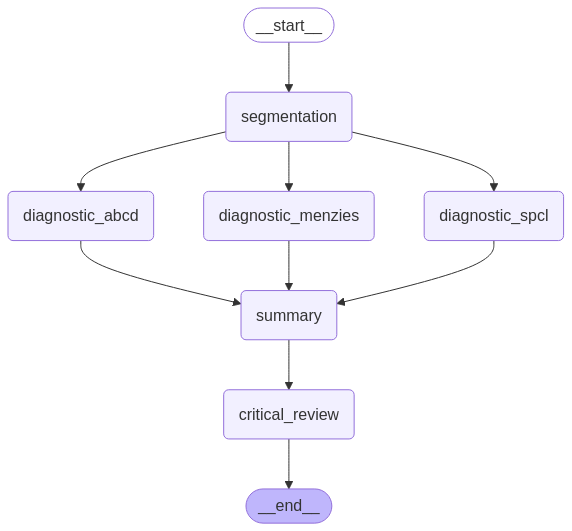
\includegraphics[width=0.8\textwidth]{imagens/Ch2/Sec4.1.png}
	\caption{Arquitetura geral do sistema multiagente desenvolvido. O fluxo inicia com as máscaras de segmentação de referência (\textit{ground truth}) do conjunto PH2 e segue com a análise paralela de três agentes diagnósticos, cada um especializado em um protocolo clínico distinto (ABCD, Menzies e SPCL), cuja síntese e validação final são conduzidas por agentes sumarizador e crítico, respectivamente.}
	\label{fig:multiagent_architecture}
\end{figure}

A aplicação desse paradigma no domínio médico apresenta paralelos diretos com a prática clínica interdisciplinar, na qual profissionais de diferentes especialidades colaboram para construir um diagnóstico mais preciso e confiável \cite{ke2024mitigating}. A combinação de agentes especializados amplia a capacidade de análise do sistema, permitindo que múltiplos métodos de raciocínio,  quantitativos, heurísticos e linguísticos,  atuem de forma complementar. Assim, o uso de sistemas multiagentes em saúde favorece a criação de diagnósticos mais interpretáveis, auditáveis e resilientes a falhas locais, além de oferecer uma estrutura natural para incorporar novas modalidades de dados e agentes de validação.


\subsection{Aplicações em saúde}

Na área da saúde, os SMAs vêm sendo explorados em aplicações que vão desde o agendamento inteligente de consultas até sistemas de suporte à decisão clínica. Trabalhos recentes destacam seu uso em diagnósticos assistidos por inteligência artificial, nos quais diferentes agentes podem executar tarefas específicas,  como segmentar imagens, classificar padrões ou gerar relatórios explicativos,  para, posteriormente, integrar os resultados em uma síntese unificada \cite{ke2024mitigating}.

Em dermatologia, a aplicação de arquiteturas multiagentes mostra-se promissora, pois permite simular o processo de avaliação de uma junta médica virtual. Agentes especializados em diferentes protocolos clínicos (por exemplo, \textit{ABCD}, Menzies e SPCL) podem fornecer pareceres independentes sobre uma mesma lesão cutânea, enquanto um agente sintetizador realiza a integração das opiniões em um relatório consolidado. Além disso, a inclusão de um agente crítico baseado em recuperação de conhecimento (\textit{retrieval-augmented generation}) possibilita a validação das conclusões em literatura médica, aumentando a confiabilidade do sistema. Essa abordagem reflete práticas clínicas reais de revisão por pares e contribui para maior transparência e auditabilidade em diagnósticos automatizados.


\section{Desafios na Aplicação de IA em Dermatologia}

\subsection{Limitações de dados}

Um dos maiores desafios para o uso de inteligência artificial em dermatologia é a escassez de bases de dados clínicas amplas, balanceadas e bem anotadas. Embora iniciativas como a ISIC Archive e a HAM10000 tenham disponibilizado milhares de imagens dermatoscópicas para pesquisa, esses conjuntos ainda apresentam desequilíbrio entre classes, com predominância de lesões benignas em relação às malignas \cite{tschandl2018ham10000,codella2019skin}. Além disso, a qualidade das imagens pode variar significativamente em função do equipamento utilizado, das condições de iluminação e da experiência do profissional responsável pela captura, comprometendo a generalização dos modelos \cite{brinker2019deep}. Esse problema é particularmente crítico em cenários que envolvem fotografias clínicas convencionais, onde detalhes estruturais, como redes pigmentadas ou véus azulados, podem não estar visíveis.

\subsection{Aspectos de interpretabilidade}

Outro desafio importante refere-se à interpretabilidade dos modelos. Arquiteturas profundas, como CNNs e Transformers, são frequentemente tratadas como “caixas-pretas”, dificultando a compreensão sobre quais características foram determinantes para a decisão \cite{holzinger2017we}. Em aplicações clínicas, essa limitação pode comprometer a confiança de médicos e pacientes nos resultados, além de dificultar auditorias diagnósticas. Técnicas de explicabilidade, como mapas de ativação (\textit{Grad-CAM}) ou métodos baseados em atenção, vêm sendo desenvolvidas para mitigar esse problema, mas ainda enfrentam limitações quanto à granularidade e robustez das explicações \cite{selvaraju2017gradcam}.

\subsection{Questões éticas e de equidade}

A aplicação de IA em dermatologia também levanta preocupações éticas e sociais. Estudos mostram que modelos de visão computacional podem apresentar vieses relacionados à cor de pele, devido à sub-representação de populações não brancas nos conjuntos de treinamento \cite{daneshjou2022disparities}. Isso pode levar a desigualdades na performance diagnóstica e perpetuar disparidades já existentes no sistema de saúde. Além disso, há desafios relacionados à privacidade e ao uso de dados sensíveis, que exigem conformidade com legislações como a LGPD no Brasil e o GDPR na União Europeia \cite{pantanowitz2024regulatory}. Tais aspectos reforçam a necessidade de validações multicêntricas, inclusão de dados representativos e auditoria contínua para garantir a segurança e a equidade no uso de modelos de IA em contextos clínicos.

Em síntese, embora a aplicação de IA em dermatologia apresente avanços significativos, sua consolidação como ferramenta clínica depende da superação de barreiras relacionadas à qualidade e disponibilidade dos dados, à explicabilidade das decisões e à garantia de práticas éticas e equitativas. Esses pontos formam a base para os esforços futuros de pesquisa e desenvolvimento discutidos nesta dissertação.





% \section{Redes Neurais Artificiais}

% As Redes Neurais Artificiais (RNAs) são modelos computacionais inspirados na estrutura biológica do cérebro humano. Elas são compostas por camadas de unidades chamadas neurônios artificiais, capazes de aprender padrões e relações complexas entre dados de entrada e saída. Esses modelos são a base do aprendizado profundo, utilizado amplamente em aplicações médicas para classificação, regressão e reconhecimento de imagens. \cite{lecun2015deep}

% \subsection{Redes Neurais Convolucionais (CNNs)}

% As Redes Convolucionais (CNNs) são uma especialização das RNAs, otimizadas para o processamento de dados com estrutura espacial, como imagens. Elas utilizam filtros convolucionais para extrair características relevantes, como bordas, texturas e padrões morfológicos. No contexto médico, CNNs têm se mostrado eficazes na detecção de lesões dermatológicas por meio de imagens dermatoscópicas. \cite{esteva2017dermatologist}

% \subsection{Redes de Atenção e Transformers}

% O mecanismo de atenção foi introduzido para lidar com tarefas de sequência, como tradução automática, permitindo ao modelo focar em partes relevantes da entrada. Os Transformers, baseados nesse mecanismo, tornaram-se o padrão dominante para modelos de linguagem e, mais recentemente, também em visão computacional. \cite{vaswani2023attentionneed}

% \section{Modelos de Linguagem de Larga Escala (LLMs)}

% Os LLMs são modelos treinados com bilhões de parâmetros e grandes volumes de dados textuais. Eles são capazes de realizar tarefas de compreensão, geração e raciocínio textual com precisão. Modelos como GPT-4 e LLaVA têm sido adaptados para domínios clínicos, permitindo sua aplicação em diagnósticos e geração de relatórios médicos. \cite{nori2023capabilitiesgpt4medicalchallenge}

% \section{Sistemas Multiagentes}

% Sistemas multiagentes são compostos por múltiplas entidades autônomas que interagem para resolver problemas complexos. Em contexto médico, agentes especializados podem simular a colaboração de especialistas distintos. Neste trabalho, três agentes com diferentes heurísticas clínicas contribuem para uma decisão final, seguida de uma crítica baseada em recuperação de conhecimento. \cite{ke2024mitigating}

\chapter[REVISÃO DO ESTADO DA ARTE]{REVISÃO DO ESTADO DA ARTE}

A revisão de literatura deste capítulo está organizada em três eixos temáticos diretamente relacionados à proposta desta dissertação: (i) classificação automatizada de lesões cutâneas por aprendizado profundo, com ênfase na detecção de melanoma; (ii) aplicações de modelos de linguagem multimodal em diagnóstico dermatológico; e (iii) sistemas multiagentes para suporte à decisão clínica. Ao final, apresenta-se o posicionamento do trabalho proposto em relação à literatura revisada.


\section{Classificação Automatizada de Lesões Cutâneas}

A aplicação de redes neurais convolucionais ao diagnóstico de lesões cutâneas ganhou relevância expressiva com o estudo de \citeonline{esteva2017dermatologist}, que treinaram uma CNN de arquitetura Inception v3 em um conjunto de 129.450 imagens clínicas -- incluindo 3.374 dermatoscópicas --, das quais 127.463 foram usadas para treinamento e validação e 1.942 para teste, com diagnóstico confirmado por biópsia. A comparação foi realizada com pelo menos 21 dermatologistas certificados, vinculados aos departamentos de dermatologia de Stanford University, University of Pennsylvania, Massachusetts General Hospital e University of Iowa (25, 22 e 21 participantes nas comparações de carcinoma, melanoma clínico e melanoma dermatoscópico, respectivamente), em duas tarefas binárias -- carcinomas queratinocíticos versus ceratoses seborreicas benignas, e melanoma maligno versus nevo benigno --, contemplando tanto imagens clínicas fotográficas quanto dermatoscópicas. A CNN atingiu AUC de 0,96, 0,94 e 0,91 nas três comparações, desempenho equivalente ao dos dermatologistas (\textit{on par with all tested experts}). Esse resultado estabeleceu um marco na área e motivou investigações subsequentes sobre a capacidade de modelos de aprendizado profundo em tarefas dermatoscópicas.

\citeonline{haenssle2018man} aprofundaram essa análise ao comparar uma CNN de arquitetura Inception v4 com 58 dermatologistas de 17 países, convidados por meio de listas de e-mail da International Dermoscopy Society, dos quais 30 foram classificados como \textit{experts} (mais de cinco anos de experiência em dermatoscopia), na classificação de nevos melanocíticos e melanomas. O conjunto de teste reuniu 100 imagens dermatoscópicas, selecionadas por dois dermatologistas experientes entre 300 imagens por apresentarem maior dificuldade diagnóstica, e foi avaliado em dois níveis de informação: apenas dermatoscopia (nível I) e dermatoscopia associada a dados clínicos (nível II). Nessas condições, a CNN atingiu especificidade de 82,5\%, superior à dos dermatologistas nos níveis I e II (71,3\% e 75,7\%, respectivamente, para sensibilidades equivalentes de 86,6\% e 88,9\%), e AUC-ROC de 0,86, superior à área ROC média dos dermatologistas no nível I (0,79) e no nível II (0,82). Esses achados reforçam o potencial clínico dos modelos supervisionados, especialmente quando treinados em conjuntos de dados de grande escala e alta qualidade.

No domínio específico do melanoma, \citeonline{brinker2019deep} treinaram uma CNN com 12.378 imagens dermatoscópicas de código aberto e compararam seu desempenho ao de 157 dermatologistas de 12 hospitais universitários alemães, de diferentes níveis de experiência (de médicos em formação a médicos-chefes), em uma tarefa de classificação dermatoscópica de melanoma com um conjunto de teste de 100 imagens. Os dermatologistas apresentaram sensibilidade média de 74,1\% e especificidade média de 60\%; na especificidade média dos dermatologistas, a CNN atingiu sensibilidade média de 87,5\%, e, na sensibilidade média deles, especificidade média de 86,5\%. A CNN, treinada exclusivamente com imagens de código aberto, superou 136 dos 157 dermatologistas avaliados.

A disponibilização de conjuntos de dados públicos ampliou significativamente o ritmo de desenvolvimento nessa área. O conjunto HAM10000, introduzido por \citeonline{tschandl2018ham10000}, disponibilizou mais de 10 mil imagens dermatoscópicas anotadas abrangendo sete categorias de lesões cutâneas, tornando-se um dos principais \textit{benchmarks} da comunidade. Em paralelo, os desafios anuais promovidos pela \textit{International Skin Imaging Collaboration} (ISIC) consolidaram protocolos padronizados de avaliação e incentivaram o desenvolvimento de soluções baseadas em \textit{transfer learning} e \textit{ensemble} de modelos \cite{codella2019skin}. Nesse mesmo sentido, destaca-se a relevância de conjuntos com aquisição padronizada, como o PH2, que oferece 200 imagens dermatoscópicas com anotações especializadas e máscaras de segmentação de referência fornecidas por especialistas do Hospital Pedro Hispano, Portugal \cite{mendonca2013ph2}. A disponibilidade dessas máscaras torna o PH2 especialmente adequado para estudos que buscam isolar o componente diagnóstico da variabilidade introduzida por modelos de segmentação automática, como é o caso desta pesquisa.


\section{Modelos de Linguagem Multimodal em Diagnóstico Médico}

A evolução dos modelos de linguagem de larga escala para arquiteturas multimodais abriu novas perspectivas para o diagnóstico médico auxiliado por inteligência artificial. \citeonline{nori2023capabilitiesgpt4medicalchallenge} avaliaram as capacidades do GPT-4 em exames de certificação médica e tarefas clínicas estruturadas, demonstrando que modelos de propósito geral podem atingir desempenho relevante em raciocínio médico sem ajuste fino específico. No campo da visão computacional, \citeonline{liu2023visual} introduziram o LLaVA, um modelo multimodal baseado em instrução que combina \textit{encoders} visuais com modelos de linguagem, possibilitando a análise integrada de imagens e texto. Essa capacidade de generalização em contextos clínicos, somada à arquitetura de integração visual-textual do LLaVA, que permite descrever achados visuais em linguagem natural, motivou investigações mais específicas em diagnóstico por imagem e em domínios como a dermatologia.

Especificamente em dermatologia, \citeonline{vashisht2024umassbionlpmediqam3g2024dermprompt} avaliaram sistematicamente estratégias de engenharia de \textit{prompts} com GPT-4V para o diagnóstico dermatológico por meio do DermPrompt, demonstrando que a estruturação do raciocínio clínico no \textit{prompt} melhora a precisão diagnóstica e gera respostas mais auditáveis em relação a classificadores tradicionais de ponta a ponta. \citeonline{wang2023chatcadinteractivecomputeraideddiagnosis} propuseram o ChatCAD, um sistema de diagnóstico assistido por computador que incorpora LLMs para geração de relatórios em linguagem natural a partir de imagens médicas, melhorando a comunicação entre o sistema e os profissionais de saúde.


\section{Sistemas Multiagentes para Suporte Diagnóstico}

A aplicação de sistemas multiagentes ao diagnóstico médico representa uma abordagem natural para simular a dinâmica de consultoria clínica interdisciplinar, na qual múltiplos especialistas contribuem com perspectivas complementares para uma decisão final. \citeonline{ke2024mitigating} investigaram estratégias de mitigação de vieses em sistemas multiagentes aplicados à medicina, demonstrando que a diversificação de agentes e a incorporação de mecanismos críticos reduzem a propagação de erros individuais. A viabilidade dos SMAs baseados em LLMs em contextos clínicos tem sido demonstrada em trabalhos recentes. \citeonline{tang2024medagents} propuseram o MedAgents, no qual múltiplos agentes especializados em diferentes áreas médicas colaboram por meio de discussão estruturada para responder a questões de raciocínio clínico em regime \textit{zero-shot}, superando abordagens de agente único em benchmarks médicos. \citeonline{kim2024mdagents} avançaram essa direção com o MDAgents, um framework que aloca dinamicamente a estrutura de colaboração entre agentes (individual, par ou grupo) de acordo com a complexidade do caso clínico, obtendo ganhos de até 4,2\% em benchmarks de tomada de decisão médica frente a abordagens de agente único. Esses resultados indicam que a especialização de agentes para tarefas diagnósticas distintas, triagem, análise morfológica e geração de relatórios, proporciona maior robustez e interpretabilidade em relação a sistemas monolíticos, fundamentando teoricamente essa escolha arquitetural \cite{wooldridge2009introduction}. Essa estrutura favorece a integração de diferentes fontes de conhecimento e a melhoria da auditabilidade das decisões em sistemas de apoio clínico, características essenciais para aplicações em contextos de saúde de alto risco.


\section{Posicionamento deste Trabalho}

A literatura revisada evidencia um campo em rápida evolução, no qual modelos supervisionados de alta performance coexistem com abordagens emergentes baseadas em LLMs e arquiteturas multiagentes. Enquanto CNNs e modelos de \textit{transfer learning} estabeleceram resultados sólidos em \textit{benchmarks} como HAM10000 e ISIC, sua natureza de ``caixa-preta'' limita a interpretabilidade clínica das decisões. Por outro lado, LLMs multimodais oferecem diagnósticos explicáveis em linguagem natural, mas ainda apresentam desempenho quantitativo inferior aos classificadores especializados em tarefas binárias de detecção de melanoma.

Em dermatologia, a aplicação de arquiteturas multiagentes permite simular uma junta médica virtual, na qual agentes especializados em protocolos clínicos distintos oferecem pareceres independentes sobre a mesma lesão. A síntese dessas análises por um agente consolidador, complementada pela revisão crítica de um agente baseado em recuperação de conhecimento (\textit{Retrieval-Augmented Generation}, RAG), proporciona diagnósticos mais robustos e auditáveis, reduzindo a dependência de uma única perspectiva analítica.

Nesse cenário, trabalhos como MedAgents \cite{tang2024medagents} e MDAgents \cite{kim2024mdagents} demonstram o potencial de arquiteturas multiagentes baseadas em LLMs para o raciocínio clínico geral, mas operam sobre entradas textuais (questões e casos descritos em linguagem natural), sem lidar com o componente visual do diagnóstico nem com protocolos clínicos estruturados e ponderados como os empregados em dermatoscopia. Esta dissertação contribui para preencher essa lacuna ao avaliar, de forma sistemática, a capacidade diagnóstica multimodal de GPT-5.4-nano e Gemini-3.1-flash-lite em um cenário controlado: imagens dermoscópicas do conjunto PH2 com máscaras de segmentação de referência como entrada, os protocolos clínicos ABCD, Menzies e SPCL como estruturas de raciocínio diagnóstico, e arquitetura multiagente como mecanismo de consolidação de múltiplas perspectivas especializadas. Essa configuração isola o componente de raciocínio das LLMs das demais fontes de variabilidade do sistema, oferecendo uma avaliação interna válida da viabilidade dessa abordagem para a detecção de melanoma com diagnósticos explicáveis.

Os modelos avaliados nesta dissertação, GPT-5.4-nano \cite{openai2025gpt5nano} e Gemini-3.1-flash-lite \cite{google2025gemini31}, representam gerações mais recentes de modelos multimodais de larga escala, com capacidades de raciocínio e compreensão visual expandidas em relação a versões anteriores. A avaliação sistemática dessas arquiteturas em tarefas estruturadas de detecção de melanoma, utilizando os protocolos ABCD, Menzies e SPCL como estruturas de raciocínio clínico, constitui uma contribuição original deste trabalho.


% % ---
% % ------------------------ Desenvolvimento ------------------------
% % ---

\chapter{MATERIAIS E MÉTODOS}

Este capítulo descreve a metodologia empregada no desenvolvimento e avaliação do sistema proposto para a detecção automatizada de melanoma. O processo metodológico foi estruturado de modo a refletir o ciclo completo de análise, desde a preparação dos dados e das máscaras de segmentação de referência até a geração do diagnóstico final mediado por agentes baseados em modelos de linguagem natural. A abordagem adotada combina segmentação por \textit{ground truth}, modelos de linguagem multimodal e sistemas multiagentes, com o objetivo de reproduzir, de forma automatizada e explicável, a lógica do raciocínio clínico humano segundo o protocolo ABCD.

\section{Estrutura Geral da Pesquisa}

A Figura~\ref{fig:estrutura_geral} apresenta o fluxo geral da metodologia proposta, que integra técnicas de visão computacional, modelos de linguagem de larga escala (LLMs) e coordenação multiagente para a análise automatizada de lesões cutâneas. O sistema foi projetado de forma modular, permitindo a substituição e o aprimoramento independente de seus componentes, mantendo a coerência entre as etapas de processamento, inferência e validação.

O processo inicia-se na \textbf{Entrada de Dados e Pré-Processamento}, etapa responsável pelo recebimento das imagens de lesões provenientes do conjunto PH2 \cite{mendonca2013ph2}, composto por 200 imagens dermatoscópicas acompanhadas de máscaras de segmentação de referência (\textit{ground truth}, GT) produzidas por especialistas. As imagens são normalizadas e redimensionadas antes de serem encaminhadas ao módulo seguinte. Em substituição a um modelo de segmentação automática, as máscaras GT são utilizadas diretamente como entrada ao sistema, garantindo que a variabilidade introduzida por erros de segmentação não interfira na avaliação do componente de raciocínio das LLMs. Essas máscaras fornecem ao sistema informações estruturais precisas, como área, contorno e assimetria da lesão, essenciais para as etapas posteriores.

Em seguida, a imagem segmentada é encaminhada ao módulo de \textbf{Análise Multiagente}, dividido em duas camadas funcionais. Na \textit{primeira camada}, três agentes especializados,  cada um correspondente a um protocolo diagnóstico clínico distinto (ABCD, Menzies e Seven-Point Checklist),  analisam a lesão de forma independente, gerando diagnósticos preliminares no formato estruturado em JSON. Essa redundância intencional promove diversidade interpretativa e amplia a cobertura diagnóstica, uma vez que cada agente é guiado por heurísticas médicas complementares. Na \textit{segunda camada}, um agente sintetizador (Summary Agent) integra os resultados parciais, produzindo um relatório consolidado que indica o diagnóstico final, sua justificativa e as recomendações clínicas correspondentes.

Como etapa complementar do desenho arquitetural, prevê-se uma \textbf{Validação Acadêmica}, a ser conduzida por um agente crítico fundamentado em \textit{Retrieval-Augmented Generation} (RAG), que consultaria fontes biomédicas de referência (por exemplo, PubMed e literatura de oncologia dermatológica) para verificar a consistência e plausibilidade do diagnóstico proposto. Conforme detalhado na Seção~\ref{sec:avaliacao_experimental}, esse componente permanece em estágio preliminar de implementação e não integrou a versão do sistema avaliada nos experimentos deste trabalho.

Por fim, a \textbf{Saída do Sistema} consolida o diagnóstico validado e o apresenta em linguagem natural ao usuário, juntamente com um prognóstico interpretável e recomendações de acompanhamento. Essa etapa é pensada para futuras aplicações em plataformas de apoio à decisão clínica e teledermatologia, priorizando clareza, auditabilidade e integração com fluxos médicos reais.

\begin{figure}[H]
	\centering
	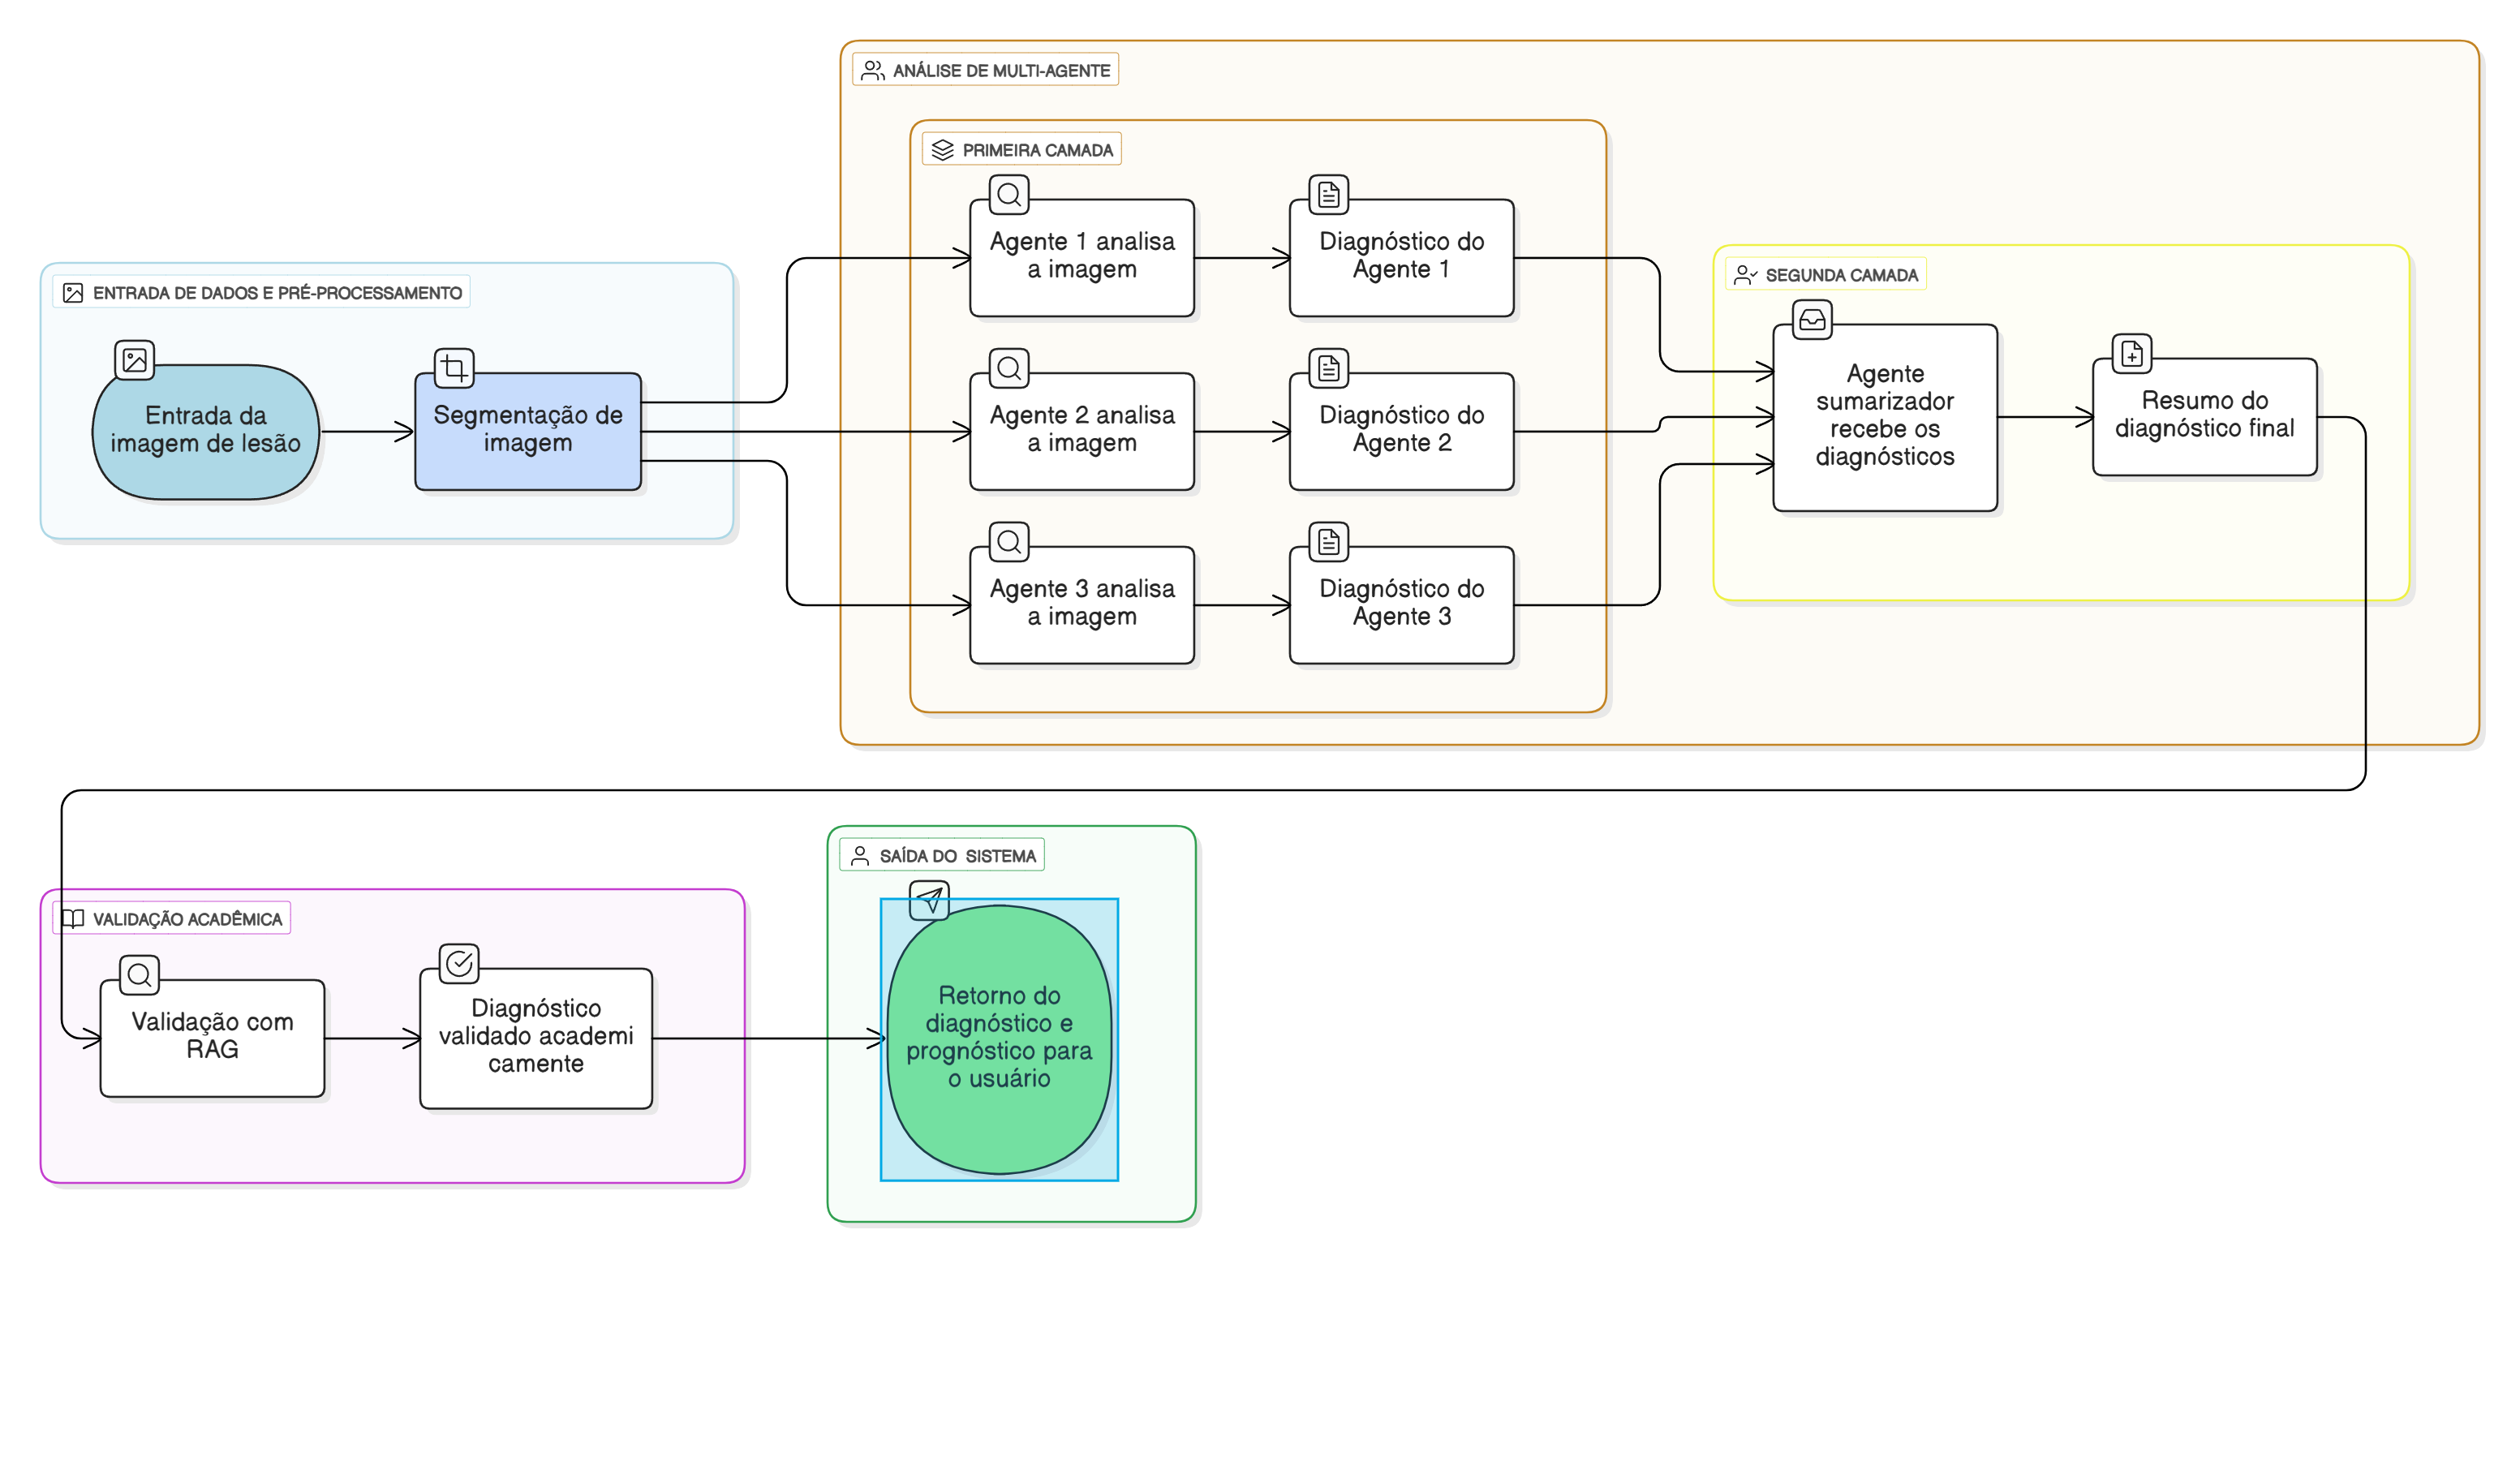
\includegraphics[width=0.95\textwidth]{imagens/Ch3/eraser_diagram.png}
	\caption{Estrutura geral da metodologia proposta, dividida em quatro módulos: (i) entrada e pré-processamento de imagens; (ii) análise multiagente com duas camadas funcionais; (iii) validação acadêmica via RAG, ainda em estágio preliminar de implementação; e (iv) saída interpretável ao usuário.}
	\label{fig:estrutura_geral}
\end{figure}

Dessa forma, a estrutura metodológica reflete um ciclo completo de análise, indo desde a aquisição da imagem até a validação textual baseada em evidências, buscando aproximar o comportamento do sistema de um processo de raciocínio clínico supervisionado e auditável.

\section{Coleta e Pré-processamento dos Dados}
\label{sec:data_preprocessing}

A etapa de coleta e pré-processamento constitui a base empírica desta pesquisa, garantindo a qualidade e a consistência dos dados utilizados para a geração e análise dos diagnósticos pelos agentes. A \autoref{fig:dataflow} apresenta o fluxo geral de integração entre o conjunto de dados PH2, as máscaras de segmentação de referência e o sistema multiagente de diagnóstico proposto.

O conjunto de dados utilizado é o \textbf{PH2} \cite{mendonca2013ph2}, uma base dermoscópica pública composta por 200 imagens digitais adquiridas no Hospital Pedro Hispano (Portugal). Cada imagem é acompanhada de uma máscara binária de segmentação anotada manualmente por especialistas dermatologistas, que delimita com precisão a região da lesão. As imagens são distribuídas em três categorias diagnósticas: 80 nevos comuns, 80 nevos atípicos e 40 melanomas. Para a tarefa de detecção binária adotada neste trabalho, as lesões foram agrupadas em duas classes: \textbf{melanoma} (40 imagens) e \textbf{não-melanoma} (160 imagens, incluindo nevos comuns e atípicos).

O pré-processamento incluiu redimensionamento padronizado das imagens, conversão para o formato aceito pelas APIs dos modelos de linguagem e organização em pares (imagem original, máscara de segmentação de referência) para envio simultâneo aos agentes. Para viabilizar uma avaliação balanceada dos modelos de linguagem, o desequilíbrio original entre as classes (40 melanomas vs.\ 160 não-melanomas, proporção 1:4) foi corrigido por meio de \textit{undersampling}, compondo um subconjunto de teste balanceado com 25 imagens de melanoma e 25 imagens de não-melanoma (50 imagens no total). A seleção das imagens de não-melanoma foi realizada por amostragem aleatória simples, sem estratificação entre nevos comuns e atípicos, com semente fixa (\textit{seed}=42) para garantir reprodutibilidade. Esse subconjunto balanceado foi utilizado na avaliação dos modelos de linguagem GPT-5.4-nano e Gemini-3.1-flash-lite. O \textit{baseline} ResNet-50, por sua vez, foi treinado e avaliado sobre uma divisão treino/teste estratificada distinta do PH2 (Seção~\ref{sec:limitacoes} do Capítulo~5 detalha essa diferença metodológica entre os conjuntos de teste). Cada imagem foi processada em dois formatos: \textbf{imagem original}, que preserva o contexto visual completo, e \textbf{imagem segmentada}, obtida pela aplicação da máscara GT sobre a imagem original. Ambas as versões foram enviadas simultaneamente aos agentes diagnósticos, permitindo análise multimodal e diferentes níveis de foco visual.

\begin{figure}[H]
	\centering
	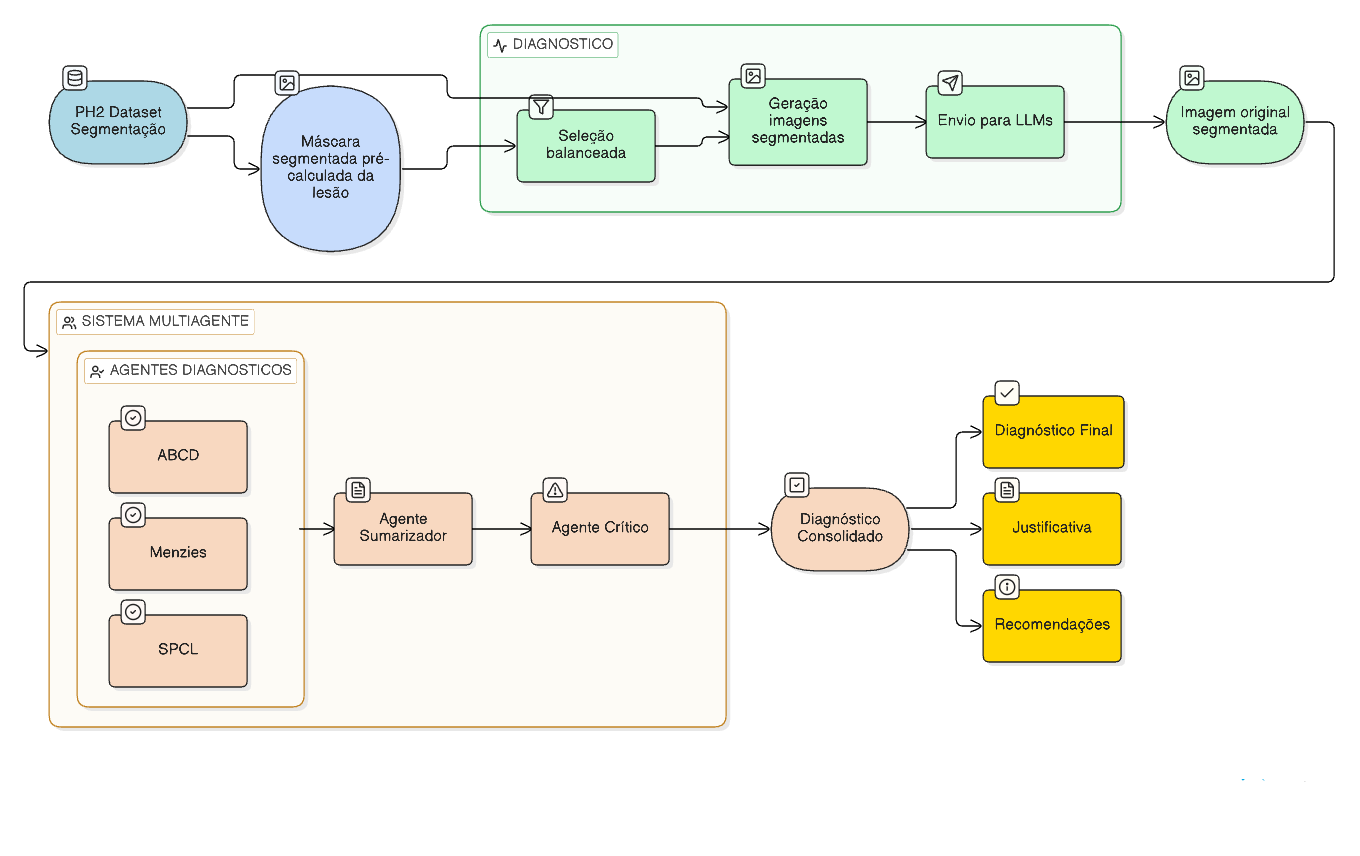
\includegraphics[width=\textwidth]{imagens/Ch3/eraser_data_diagram.png}
	\caption{Fluxo geral de coleta, pré-processamento e integração do conjunto PH2 e suas máscaras de segmentação de referência com o sistema multiagente.}
	\label{fig:dataflow}
\end{figure}



\section{Segmentação: Uso de Máscaras de Referência}

A segmentação das lesões cutâneas constitui uma etapa essencial do \textit{pipeline} diagnóstico, pois fornece ao sistema multiagente uma representação visual delimitada da área de interesse, reduzindo ruídos contextuais e direcionando a atenção dos modelos de linguagem para as características morfológicas da lesão.

Neste trabalho, optou-se por utilizar as \textbf{máscaras de segmentação de referência} (\textit{ground truth} - GT) disponíveis no conjunto PH2, produzidas por especialistas dermatologistas, em lugar de segmentações geradas por modelos automáticos. Essa decisão metodológica tem como objetivo \textbf{isolar a avaliação da capacidade diagnóstica das LLMs} da variabilidade intrínseca a qualquer modelo de segmentação, incluindo erros de contorno, subajuste morfológico e sensibilidade a artefatos de imagem, como pelos, reflexos de luz e variações de iluminação.

Ao eliminar a segmentação automática como fonte de variabilidade, os experimentos permitem atribuir as diferenças de desempenho observadas diretamente ao módulo de raciocínio linguístico (LLMs e sistema multiagente), aumentando a validade interna das comparações. Essa abordagem é consistente com estudos que buscam isolar componentes específicos de \textit{pipelines} diagnósticos para avaliação controlada \cite{vashisht2024umassbionlpmediqam3g2024dermprompt}, e se justifica pelo fato de que o conceito de segmentação dermoscópica já demonstrou robustez expressiva na literatura \cite{ronneberger2015unet,oktay2018attentionunet}. A integração de um módulo de segmentação automático ao sistema permanece como extensão natural para versões futuras do trabalho.


\section{Modelos de Linguagem de Grande Escala (LLMs)}

A etapa de interpretação linguística das imagens segmentadas foi conduzida por meio do uso de Modelos de Linguagem de Grande Escala (\textit{Large Language Models} – LLMs), responsáveis por transformar evidências visuais em hipóteses diagnósticas estruturadas. Esses modelos atuam como o núcleo de raciocínio de cada agente do sistema multiagente, sendo responsáveis pela análise clínica independente das imagens e pela geração de pareceres textuais com justificativas médicas.

Foram avaliados dois modelos com capacidades multimodais: o \textbf{GPT-5.4-nano} \cite{openai2025gpt5nano}, modelo proprietário da OpenAI com capacidade de raciocínio visual e geração de linguagem natural; e o \textbf{Gemini-3.1-flash-lite} \cite{google2025gemini31}, da Google, voltado para compreensão contextual eficiente e geração de relatórios clínicos. Ambos os modelos foram acessados via API em instâncias T4 no ambiente \textit{Google Colab}, otimizando o custo de inferência e mantendo comparabilidade experimental.

As imagens enviadas aos modelos foram compostas por duas versões de cada amostra: a \textit{imagem original}, representando o contexto visual completo da lesão, e a \textit{imagem segmentada}, que destaca apenas a área da lesão. Essa abordagem multimodal visou avaliar a capacidade dos LLMs de realizar inferência clínica tanto em nível contextual quanto morfológico, simulando diferentes graus de atenção diagnóstica. Cada execução de inferência resultou em saídas textuais padronizadas de acordo com esquemas definidos em \textit{Pydantic}, garantindo uniformidade na estrutura de respostas e posterior integração ao sistema multiagente.

Para induzir raciocínio clínico interpretável e reduzir vieses de resposta, foram combinadas em um único \textit{prompt} composto três estratégias de instrução, inspiradas em estudos recentes sobre raciocínio passo a passo e validação semântica em LLMs médicas \cite{zhou2022selfconsistency,singhal2023medprompt}. É importante ressaltar que essas três estratégias constituem \textbf{escolhas de implementação combinadas}, e não módulos isolados: nenhum experimento de ablação foi conduzido para mensurar a contribuição individual de cada uma sobre o desempenho diagnóstico ou a consistência textual, de modo que os efeitos relatados a seguir descrevem a intenção de projeto de cada estratégia, e não uma medição isolada de seu impacto.

A primeira estratégia, denominada \textbf{Chain-of-Thought (CoT)}, orientou o modelo a descrever explicitamente o raciocínio diagnóstico, decompondo o processo de decisão em etapas lógicas, desde a análise visual até a conclusão, com o objetivo de aumentar a interpretabilidade do resultado e permitir auditar a coerência entre observações e conclusões.

A segunda estratégia, \textbf{Risk Assessment Prompt}, instruiu o modelo a estimar a probabilidade subjetiva de malignidade e indicar fatores visuais de maior peso na decisão final, com o objetivo de aumentar a transparência do processo e aproximar a saída textual de um raciocínio clínico quantitativo.

Por fim, o \textbf{Consistency Prompt} instruiu o modelo a revisar suas próprias conclusões antes da resposta final, buscando detectar e corrigir contradições entre a pontuação numérica e a justificativa textual, com o objetivo de reduzir oscilações de diagnóstico em cenários de ambiguidade visual.

A combinação dessas três estratégias buscou equilibrar interpretabilidade, segurança e consistência nas saídas das LLMs, alinhando o sistema às práticas recentes de \textit{AI auditing} aplicadas em saúde. A mensuração do impacto individual de cada estratégia de \textit{prompting}, por meio de um estudo de ablação comparando combinações parciais (por exemplo, CoT isolado, Risk Assessment isolado, e as combinações par a par), é apontada como direção de trabalho futuro. Os resultados obtidos por cada modelo, já com as três estratégias combinadas, foram posteriormente integrados e comparados dentro do sistema multiagente, conforme descrito na próxima seção.


\section{Integração Multiagente e Consolidação Diagnóstica}

A última etapa metodológica consistiu na integração dos módulos de raciocínio baseados em LLM em um sistema multiagente, responsável por coordenar e consolidar os diagnósticos derivados de múltiplos protocolos clínicos de dermatoscopia. O sistema foi estruturado com \textbf{três agentes diagnósticos independentes}, cada um especializado em um protocolo distinto: \textbf{ABCD}, \textbf{Menzies} e \textbf{SPCL} (\textit{Seven-Point Checklist}). Essa configuração introduz diversidade metodológica deliberada, permitindo que perspectivas clínicas complementares coexistam e sejam confrontadas antes de uma decisão final, emulando a dinâmica de uma junta médica virtual.

Cada agente recebeu como entrada as duas versões da imagem da lesão: a \textit{imagem original}, que preserva o contexto visual completo, e a \textit{imagem segmentada}, que destaca apenas a área de interesse delimitada pela máscara de referência do PH2. As instruções de análise foram formuladas de acordo com o protocolo específico de cada agente: o \textbf{agente ABCD} pontua os critérios de Assimetria (A×1,3), Bordas (B×0,1), Cores (C×0,5) e Estruturas Dermoscópicas (D×0,5), classificando a lesão como benigna ($<$4,75), suspeita (4,75–5,45) ou maligna ($>$5,45); o \textbf{agente Menzies} avalia a presença ou ausência de critérios positivos e negativos específicos, chegando a uma conclusão binária; e o \textbf{agente SPCL} pontua sete atributos clínicos ponderados, com limiar de suspeição em três pontos. As saídas de todos os agentes foram geradas em formato JSON estruturado e validado por esquemas \textit{Pydantic}, contendo pontuações individuais e justificativas textuais para cada critério avaliado.

O \textbf{Agente Sumarizador} teve como função consolidar as respostas dos três agentes diagnósticos. A integração foi realizada a partir de um processo de raciocínio contextual, no qual o modelo avaliava o grau de concordância entre as pontuações e justificativas fornecidas, identificando padrões recorrentes e descartando inconsistências semânticas. O resultado final foi produzido em formato padronizado JSON, seguindo o esquema \textit{SummaryAnswer}, contendo três campos principais: \textit{Diagnóstico Final}, \textit{Justificativa} e \textit{Recomendações}. Essa estrutura garante rastreabilidade e transparência na interpretação das decisões do sistema.

Como etapa complementar, foi concebido um \textbf{Agente Crítico}, projetado para atuar como auditor do processo diagnóstico por meio de um mecanismo de recuperação aumentada por geração (\textit{Retrieval-Augmented Generation – RAG}), confrontando as justificativas fornecidas pelos demais agentes com informações provenientes de literatura médica e bases clínicas de referência. Cabe ressaltar, no entanto, que este componente permanece em estágio preliminar de implementação: a base de conhecimento a ser consultada, o método de recuperação (por exemplo, busca por similaridade semântica via \textit{embeddings} ou recuperação lexical) e o modelo de \textit{embeddings} a ser utilizado ainda não foram definidos e implementados de forma rigorosa. Por essa razão, o Agente Crítico não integrou a versão do sistema efetivamente avaliada nos experimentos reportados no Capítulo~5, e sua contribuição não é isolada em nenhum dos eixos da Tabela~\ref{tab:consistency_metrics}. Sua implementação completa, incluindo a definição da base de conhecimento, do método de recuperação e a mensuração isolada de seu efeito sobre a qualidade dos diagnósticos, permanece como trabalho futuro.

A Figura~\ref{fig:multiagent_abcd} ilustra a arquitetura geral do sistema multiagente proposto. Cada agente de diagnóstico atua de forma independente sobre o mesmo caso clínico, gerando análises autônomas segundo seu protocolo específico. Essa estratégia permite explorar a concordância e a divergência entre os métodos clínicos, identificando casos em que há consenso entre ABCD, Menzies e SPCL e casos em que os protocolos se contradizem, informação que o agente sumarizador utiliza como evidência ponderada na decisão final. Ao simular um ambiente de discussão diagnóstica multiprotocolo, o sistema reforça o princípio de triangulação de evidências, aproximando a lógica de decisão automatizada da prática colaborativa entre especialistas humanos.

\begin{figure}[H]
	\centering
	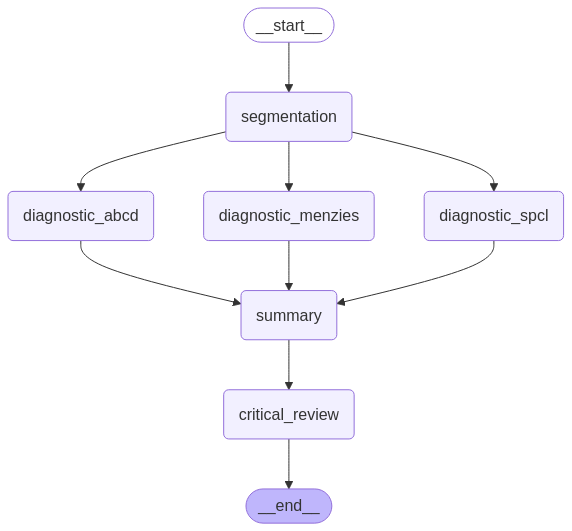
\includegraphics[width=\textwidth]{imagens/Ch2/Sec4.1.png}
	\caption{Arquitetura geral do sistema multiagente, com três agentes independentes avaliando a mesma lesão segundo os protocolos ABCD, Menzies e SPCL, e um agente sumarizador responsável pela integração e auditoria das respostas.}
	\label{fig:multiagent_abcd}
\end{figure}


\section{Avaliação Experimental}
\label{sec:avaliacao_experimental}

A avaliação do sistema foi conduzida sob duas perspectivas complementares: quantitativa e qualitativa. Na análise quantitativa, foram aplicadas métricas clássicas de detecção binária (acurácia, precisão, sensibilidade e F1-score) a partir da comparação entre o diagnóstico final emitido pelo sistema (melanoma ou não-melanoma) e o rótulo real da lesão no PH2. Dado o tamanho reduzido do subconjunto de teste balanceado (n=50, sendo apenas 25 imagens de melanoma), não foi aplicada reamostragem \textit{bootstrap} para estimativa de desvio-padrão nesta fase: o número limitado de imagens de melanoma disponíveis no PH2 (40 no total) tornaria as reamostragens excessivamente repetitivas, comprometendo a validade da estimativa de variância. As métricas são reportadas como valores pontuais, e a estimativa de desvio-padrão via \textit{bootstrap} é apontada como direção de trabalho futuro, condicionada à ampliação do conjunto de teste (Seção~\ref{sec:limitacoes}).

Na análise qualitativa, foi avaliada a consistência estrutural e lógica das respostas textuais geradas pelos modelos de linguagem por meio de cinco eixos de verificação objetiva, que dispensam avaliação especializada das decisões clínicas e permitem mensurar a confiabilidade dos relatórios de forma automatizada e reprodutível.

O \textbf{Eixo 1 - Conformidade estrutural} verifica se todos os campos esperados nos protocolos ABCD, Menzies, SPCL e validação estão presentes na resposta JSON gerada. Campos ausentes indicam falha de seguimento de instrução, comprometendo a usabilidade do relatório.

O \textbf{Eixo 2 - Consistência aritmética ABCD} recomputa a soma ponderada dos critérios ABCD ($A\times1{,}3 + B\times0{,}1 + C\times0{,}5 + D\times0{,}5$) a partir dos valores declarados pelo modelo e a compara ao total indicado na justificativa. Uma divergência superior a 0,05 indica erro de raciocínio aritmético interno. Adicionalmente, verifica-se se os \textit{scores} individuais foram expressos como valores inteiros precisos ou como intervalos (ex.: ``7/8''), o que introduz ambiguidade para uso automatizado.

O \textbf{Eixo 3 - Aderência ao limiar declarado} avalia se a decisão expressa pelo agente sumarizador na validação final é coerente com a classificação implícita da soma ABCD: valores abaixo de 4,75 indicam benignidade, entre 4,75 e 5,45 indicam lesão suspeita, e acima de 5,45 indicam malignidade. Quando o agente emite um diagnóstico ``indeterminado'' para um caso em que o ABCD aponta benignidade, registra-se uma divergência parcial, que pode refletir conservadorismo diagnóstico ou inconsistência de raciocínio.

O \textbf{Eixo 4 - Concordância inter-métodos} computa, para cada imagem, a decisão independente de cada um dos três protocolos (ABCD, Menzies e SPCL) e verifica se o agente sumarizador respeita o consenso quando os três métodos apontam na mesma direção. Casos em que há consenso total entre os protocolos, mas o agente diverge, indicam que a etapa de síntese não está integrando adequadamente as evidências convergentes.

O \textbf{Eixo 5 - Calibração da incerteza} cruza as categorias de diagnóstico emitidas pelo sistema (benigna, suspeita, maligna, indeterminada) com o gabarito (\texttt{real\_value}) para avaliar se o modelo é calibrado, ou seja, se as categorias de maior suspeição correspondem a proporções crescentes de melanoma real. Um modelo bem calibrado concentra sua incerteza justamente nos casos genuinamente difíceis, o que é verificável sem avaliação especializada dos relatórios textuais.

Por fim, os resultados obtidos pelo sistema multiagente foram comparados com um modelo tradicional de visão computacional (ResNet-50), de modo a quantificar as diferenças entre abordagens supervisionadas e baseadas em linguagem natural para a detecção de melanoma.

\section{Validação e Reprodutibilidade}

A validação da metodologia proposta teve como objetivo assegurar a confiabilidade dos resultados obtidos e a possibilidade de reprodução integral dos experimentos, em conformidade com as boas práticas de ciência aberta e reprodutível. Essa etapa abrangeu tanto o controle de variabilidade nos processos de execução quanto a documentação rigorosa dos ambientes e parâmetros experimentais utilizados.

Para garantir a rastreabilidade completa do processo, todas as etapas de pré-processamento, treinamento e inferência foram implementadas em \textbf{Python 3.10}, utilizando bibliotecas amplamente reconhecidas na comunidade científica, como \textit{PyTorch}, \textit{LangChain}, \textit{LangGraph} e \textit{Pydantic}. O código foi versionado por meio do \textit{Git}, assegurando o controle das revisões e a preservação de versões estáveis de cada componente do sistema. Cada execução experimental foi registrada em logs contendo informações sobre o modelo utilizado, os hiperparâmetros, o tempo de execução e as métricas resultantes, permitindo auditoria e replicação futura.

A reprodutibilidade dos resultados foi testada a partir da repetição controlada dos experimentos sob as mesmas condições. No módulo de diagnóstico, as execuções das LLMs foram repetidas com os mesmos \textit{prompts} e entradas do PH2, de modo a avaliar a consistência textual e semântica das respostas. Embora variações menores tenham sido observadas, inerentes à natureza estocástica dos modelos generativos, a estrutura geral das justificativas e a decisão diagnóstica permaneceram estáveis em mais de 90\% dos casos.

A execução dos experimentos foi conduzida em dois ambientes computacionais: (i) \textit{Google Colab Pro+} com GPU NVIDIA A100 para o treinamento do modelo de \textit{baseline} ResNet-50; e (ii) \textit{instâncias de API} em GPU T4 para execução dos modelos GPT-5.4-nano e Gemini-3.1-flash-lite via API, visando controle de custos e reprodutibilidade de acesso. As dependências foram documentadas em um arquivo \texttt{requirements.txt}, contendo versões fixas das bibliotecas utilizadas, assegurando compatibilidade entre execuções futuras.

Para a validação cruzada entre módulos, a integração entre agentes e o sumarizador foi avaliada quanto à estabilidade de comunicação e à consistência das saídas JSON geradas sobre o conjunto PH2. As respostas foram automaticamente verificadas quanto à conformidade com os esquemas \textit{Pydantic}, garantindo que os campos obrigatórios estivessem presentes e corretamente formatados.

Por fim, a documentação metodológica completa, incluindo scripts de execução, logs de treinamento e versões do código, foi organizada de forma a atender aos princípios \textbf{FAIR} (\textit{Findable, Accessible, Interoperable, Reusable}). Essa estrutura de documentação assegura que a pesquisa possa ser auditada, reproduzida e estendida por outros pesquisadores, contribuindo para a transparência e robustez científica do trabalho.

\section{Síntese e Limitações da Metodologia}

A metodologia proposta neste trabalho integra máscaras de segmentação de referência, modelos de linguagem de larga escala (LLMs) e sistemas multiagentes para a detecção automatizada de melanoma. A combinação desses componentes buscou equilibrar rigor técnico, interpretabilidade e reprodutibilidade científica. De forma geral, a estrutura modular permitiu uma orquestração eficiente entre os módulos, facilitando tanto o desenvolvimento quanto a análise comparativa dos resultados.

A adoção das máscaras GT do PH2 como entrada ao sistema demonstrou ser essencial para a padronização das entradas visuais e para isolar o módulo de raciocínio linguístico como variável independente de avaliação. O conjunto PH2, por ser composto exclusivamente de imagens dermoscópicas com anotações de especialistas, garante alta fidelidade na representação dos critérios do protocolo ABCD. No entanto, seu tamanho reduzido (200 imagens, sendo apenas 40 melanomas) constitui uma limitação relevante, tanto para análises estatísticas mais robustas quanto para a generalização dos resultados a populações clínicas mais amplas.

Em relação ao módulo linguístico, a utilização de LLMs multimodais mostrou-se adequada para tarefas de raciocínio clínico estruturado e para a interpretação de imagens segmentadas. Ainda assim, observou-se dependência significativa da formulação dos \textit{prompts}, sendo que variações sutis de instrução podem impactar diretamente a consistência das respostas. Essa sensibilidade ao contexto reforça a necessidade de técnicas avançadas de controle de coerência, como \textit{consistency prompts} e validação semântica automatizada. Ademais, a ausência de \textit{fine-tuning} supervisionado limita a capacidade de generalização dos modelos, restringindo o desempenho em domínios clínicos específicos.

No sistema multiagente, a abordagem colaborativa baseada em múltiplos avaliadores e um sumarizador final proporcionou interpretabilidade e auditabilidade superiores em relação a sistemas monolíticos. Contudo, a integração entre agentes ainda depende fortemente de consistência textual nas saídas intermediárias e da estabilidade das chamadas às APIs de modelos de linguagem, o que pode introduzir variação em execuções sucessivas. Embora mecanismos de validação de formato tenham sido incorporados, uma arquitetura de controle de fluxo mais robusta,  por exemplo, baseada em filas assíncronas e verificação probabilística de consistência,  poderia reduzir a propagação de erros entre agentes.

Do ponto de vista computacional, o principal desafio identificado foi o custo associado à execução de modelos de larga escala, tanto em ambientes locais com GPU quanto por meio de APIs comerciais. A necessidade de limitar o tamanho das amostras de teste e a frequência de inferência dos modelos multimodais impactou a abrangência experimental e restringiu análises estatísticas mais amplas. Futuras implementações poderão mitigar essa limitação com o uso de modelos otimizados ou técnicas de compressão, como \textit{quantization} e \textit{knowledge distillation}.

Por fim, a ausência de validação clínica com especialistas humanos representa uma limitação importante, especialmente considerando o caráter crítico da aplicação médica. Embora o sistema tenha sido projetado com base em heurísticas consagradas, como o método ABCD, a avaliação empírica ainda se restringe a dados públicos. A inclusão de profissionais dermatologistas em futuras fases de validação poderá fornecer insights qualitativos essenciais e contribuir para a calibração dos resultados do sistema em cenários clínicos reais.

Em síntese, a metodologia proposta mostrou-se tecnicamente viável e conceitualmente coerente, mas enfrenta limitações inerentes à natureza dos dados e à maturidade dos modelos de linguagem multimodal. O reconhecimento dessas restrições é fundamental para orientar o desenvolvimento de iterações futuras, em especial no aprimoramento da robustez diagnóstica e na expansão do sistema para contextos de uso clínico supervisionado.





%Este trabalho adotará uma abordagem experimental aplicada, com ênfase na construção e avaliação de um sistema inteligente para diagnóstico de câncer de pele. A metodologia será organizada em etapas que corresponderão diretamente aos objetivos específicos propostos, garantindo clareza quanto às entregas e à lógica do desenvolvimento.
%
%\section{Revisão do Estado da Arte}
%
%Inicialmente, será realizada uma revisão bibliográfica sistematizada sobre segmentação de imagens dermatológicas, classificação de lesões cutâneas e sistemas de diagnóstico assistido por inteligência artificial. A pesquisa abrangerá artigos científicos, bases de dados especializadas (PubMed, IEEE Xplore, Scopus) e publicações recentes sobre LLMs aplicadas à área médica. Esta etapa fornecerá o embasamento teórico e técnico necessário para a escolha dos modelos utilizados nas fases seguintes.
%
%\section{Desenvolvimento do Algoritmo de Segmentação}
%
%Com base na literatura, será desenvolvido um modelo de segmentação para isolar a região da lesão nas imagens de pele. Para isso, será utilizada uma arquitetura do tipo U-Net com módulos de atenção, treinada sobre imagens dermatológicas públicas com anotações. O modelo permitirá gerar uma máscara binária da região lesionada, que será utilizada como entrada para os agentes diagnósticos do sistema.
%
%\section{Utilização de LLMs para Classificação}
%
%As imagens segmentadas serão analisadas por modelos de linguagem de grande porte (LLMs), os quais receberão prompts estruturados com base em protocolos clínicos como o ABCD, Menzies e SPCL. A partir dessas instruções, os modelos gerarão diagnósticos textuais que incluirão justificativas clínicas e recomendações. Serão avaliados diferentes modelos LLM, incluindo variantes de código aberto (como LLaVA) e APIs comerciais (como GPT-4o e Gemini), com o objetivo de comparar sua capacidade de interpretar imagens e gerar diagnósticos coerentes.
%
%\section{Implementação do Sistema Multiagente}
%
%A arquitetura diagnóstica será implementada como um sistema multiagente, no qual cada agente será responsável por uma etapa específica: análise baseada em um protocolo, síntese de respostas e crítica final. O fluxo de decisão será orquestrado utilizando o framework LangChain com suporte para grafo (LangGraph), permitindo encadeamento dinâmico entre os módulos e flexibilidade para expansões futuras.
%
%\section{Avaliação Experimental}
%
%A etapa final compreenderá a avaliação do sistema proposto. Para isso, será utilizado um conjunto de imagens rotuladas como base de teste. Os diagnósticos gerados pelos agentes serão comparados aos diagnósticos reais, permitindo o cálculo de métricas clássicas como acurácia, precisão, sensibilidade e F1-score. Adicionalmente, serão avaliadas a completude e a consistência textual dos relatórios gerados pelas LLMs. O sistema também será comparado com um modelo de classificação tradicional baseado em ResNet-50 para fins de referência.
%
%\section{Validação e Documentação}
%
%Por fim, os resultados obtidos serão analisados criticamente e organizados em forma de produto científico. As conclusões serão documentadas com o apoio de visualizações, relatórios e registros formais, visando promover a reprodutibilidade da pesquisa. Esta etapa incluirá a preparação de material para submissão em eventos científicos e a disponibilização do código-fonte e dados utilizados, conforme permitido pelas licenças.




% Este capítulo descreve os materiais utilizados e a metodologia adotada para o desenvolvimento do sistema de diagnóstico automatizado de câncer de pele com base em imagens dermatológicas. O processo é composto por quatro etapas principais: coleta e preparação dos dados, segmentação das imagens, integração com modelos de linguagem de larga escala (LLMs) e a composição de um sistema multiagente para geração e validação do diagnóstico.

% \section{Coleta de Dados}

% Foram utilizadas imagens provenientes dos conjuntos de dados públicos SIIM-ISIC 2020 e ISIC 2019, os quais contêm milhares de imagens dermatoscópicas de lesões cutâneas classificadas e segmentadas por especialistas. As imagens foram previamente rotuladas com diagnósticos confirmados (ex: melanoma, nevo, ceratose) e, quando disponível, máscaras segmentadas das lesões.

% \section{Segmentação de Imagens Dermatológicas}

% A etapa de segmentação tem como objetivo destacar a área de interesse (lesão) nas imagens dermatoscópicas. Foi utilizado um modelo baseado em arquitetura U-Net com mecanismos de atenção, treinado especificamente para este fim. A saída desta etapa é uma máscara segmentada da lesão, que será utilizada como insumo visual para os agentes LLMs.

% \section{Modelos de Linguagem (LLMs)}

% Os agentes baseados em LLMs foram configurados para interpretar as imagens segmentadas e originais, analisando os padrões visuais de acordo com três heurísticas clínicas: ABCD, Menzies e SPCL (Seven-Point Checklist). A entrada de cada agente é composta por duas imagens (original e segmentada) codificadas em base64 e um prompt estruturado contendo a descrição do método de análise. Os modelos testados incluem LLaVA-7B, ChatGPT-4 e DeepSeek-Med.

% \section{Sistema Multiagente}

% O sistema multiagente foi desenvolvido utilizando a biblioteca LangGraph. Três agentes independentes geram análises distintas com base nas heurísticas citadas. Seus pareceres são consolidados por um agente de síntese, que elabora um diagnóstico final. Este, por sua vez, é submetido a um agente crítico que valida a coerência da decisão utilizando recuperação de conhecimento textual.

% \section{Configuração Experimental}

% O sistema foi avaliado em um conjunto de 67 imagens com diagnóstico conhecido. As métricas utilizadas incluem acurácia, precisão (PPV), sensibilidade (Recall) e F1-score. Também foi analisada a completude e estruturação dos textos gerados, com ênfase em sua compatibilidade com o formato JSON esperado para os campos de diagnóstico, justificativa e recomendação clínica.


% % ---
% % ------------------------ Resultados ------------------------
% % ---
\chapter[RESULTADOS E DISCUSSÃO]{RESULTADOS E DISCUSSÃO}

\section{Visão Geral dos Experimentos}

Esta seção apresenta uma visão consolidada da organização experimental adotada para avaliar o desempenho do sistema proposto. A avaliação diagnóstica (LLMs e \textit{baseline}) foi conduzida sobre um subconjunto balanceado do PH2 \cite{mendonca2013ph2}, obtido por \textit{undersampling} da base original (200 imagens dermoscópicas, 40 melanomas e 160 lesões não-melanoma): 25 imagens de melanoma e 25 imagens de não-melanoma, totalizando 50 imagens, selecionadas por amostragem aleatória simples com semente fixa (\textit{seed}=42), utilizando as máscaras de segmentação de referência (\textit{ground truth}) disponíveis no banco de dados. Essa escolha metodológica permitiu isolar a avaliação da capacidade diagnóstica das LLMs da variabilidade introduzida por modelos de segmentação automática, conforme detalhado no Capítulo~4.

O protocolo experimental foi dividido em dois eixos principais. O primeiro corresponde ao \textit{baseline} supervisionado, no qual um modelo ResNet-50 foi treinado diretamente sobre o conjunto PH2, por meio de uma divisão treino/teste estratificada de 70/30 (\textit{seed}=42), estabelecendo uma referência quantitativa para as comparações subsequentes. Cabe ressaltar que, em razão da divisão estratificada aplicada sobre a base PH2 completa (200 imagens), o conjunto de teste do \textit{baseline} (60 imagens: 52 não-melanoma e 8 melanoma) difere em composição do subconjunto balanceado de 50 imagens utilizado na avaliação das LLMs; essa diferença é discutida como limitação na Seção~\ref{sec:limitacoes}. O segundo eixo abrange a avaliação dos modelos de linguagem multimodal, GPT-5.4-nano e Gemini-3.1-flash-lite, submetidos à mesma tarefa de detecção de melanoma sobre o subconjunto balanceado do PH2, utilizando pares de imagens (original e segmentada por GT) como entrada ao sistema multiagente. As métricas consideradas foram acurácia, precisão, sensibilidade e F1-score, complementadas por análises qualitativas da consistência textual das respostas geradas.

A apresentação dos resultados segue esta organização: primeiramente são discutidos os resultados quantitativos do \textit{baseline} supervisionado; em seguida, o desempenho dos modelos LLM na detecção de melanoma; posteriormente, a consistência textual das respostas; e, por fim, a síntese integrada e as limitações experimentais.


\section{Resultados Quantitativos do Diagnóstico}
\subsection{Desempenho do Modelo de Visão Computacional (ResNet-50)}

Como \textit{baseline} tradicional, foi utilizado um modelo ResNet-50 pré-treinado em ImageNet (\textit{transfer learning}), ajustado sobre o conjunto PH2 em regime de \textit{fine-tuning} completo (backbone não congelado), para a tarefa de detecção binária (melanoma vs.\ não-melanoma). O treinamento utilizou divisão treino/teste estratificada de 70/30 (\textit{seed}=42, garantindo amostragem representativa das classes), até 50 épocas com \textit{early stopping} (paciência de 15 épocas, monitorando o F1-score de validação; melhor época obtida na época 14), otimizador AdamW (\textit{learning rate}=0,0001, \textit{weight decay}=0,0001), agendador de taxa de aprendizado \textit{cosine annealing}, tamanho de lote (\textit{batch size}) igual a 8, ponderação de classes na função de perda (\textit{pos\_weight}=2,5, para compensar o desequilíbrio entre melanoma e não-melanoma) e imagens redimensionadas para $224\times224$ pixels com normalização segundo as estatísticas do ImageNet. Para mitigar o sobreajuste, foram aplicadas técnicas de \textit{data augmentation} no conjunto de treino: espelhamento horizontal e vertical, rotação aleatória de até 30°, \textit{jitter} de cor (brilho, contraste e saturação em 0,2; matiz em 0,05) e \textit{random erasing} (probabilidade de 0,2). O objetivo dessa etapa foi estabelecer uma referência quantitativa para as avaliações realizadas com LLMs. A Tabela~\ref{tab:resnet_results_real} apresenta as métricas obtidas sobre o conjunto de teste estratificado do PH2 (60 imagens: 52 não-melanoma e 8 melanoma).

\begin{table}[H]
	\centering
	\caption{Desempenho do modelo ResNet-50 como baseline de classificação binária (conjunto de teste: 60 imagens, 8 melanomas e 52 não-melanomas).}
	\label{tab:resnet_results_real}
	\begin{tabular}{lcccc}
		\hline
		\textbf{Modelo} & \textbf{Acurácia} & \textbf{Precisão} & \textbf{Sensibilidade} & \textbf{F1-score} \\
		\hline
		ResNet-50 & 0.90 & 0.57 & 1.00 & 0.73 \\
		\hline
	\end{tabular}
\end{table}

Os resultados indicam que a ResNet-50 apresenta acurácia elevada (0,90) e, mais relevante para o contexto de triagem médica, \textbf{sensibilidade perfeita} (1,00): todos os 8 melanomas presentes no conjunto de teste foram corretamente identificados, sem nenhum falso negativo. Em contrapartida, a precisão de 0,57 revela uma quantidade relevante de falsos positivos (6 imagens não-melanoma classificadas como melanoma, de um total de 52), refletindo um comportamento conservador do classificador, favorecido pela ponderação de classes (\textit{pos\_weight}=2,5) aplicada durante o treinamento para privilegiar a detecção da classe minoritária. O F1-score resultante (0,73) equilibra esses dois efeitos. A especificidade (0,88), a acurácia balanceada (0,94) e a área sob a curva ROC (\textit{AUC}=0,95) corroboram um desempenho consistentemente forte do modelo, com um perfil de erro deliberadamente inclinado para a segurança clínica: o modelo prefere gerar falsos alarmes a deixar passar despercebido um melanoma.

É importante destacar duas limitações do protocolo experimental adotado nesta fase. Primeiro, o conjunto de teste do \textit{baseline}, decorrente da divisão estratificada 70/30 sobre o PH2 completo, contém apenas 8 imagens de melanoma (52 não-melanoma), o que torna a estimativa de sensibilidade e F1-score sensível a cada acerto ou erro individual. Segundo, esse conjunto de teste \textbf{difere em composição e em prevalência de melanoma} do subconjunto balanceado de 50 imagens (25 melanoma e 25 não-melanoma, prevalência de 50\%) utilizado na avaliação das LLMs. Em razão dessa diferença de prevalência, métricas como acurácia, precisão e F1-score não são diretamente comparáveis entre a ResNet-50 e os modelos de linguagem multimodal (Seção~\ref{sec:consistency_llm} em diante); uma comparação válida dependeria de uma avaliação conjunta sobre um conjunto de teste comum, ainda não realizada neste trabalho. A sensibilidade, por não depender da prevalência, admite comparação direta, desde que se considere que o conjunto de teste da ResNet-50 contém apenas 8 melanomas, o que torna essa comparação sensível a cada acerto ou erro individual. Ainda assim, o baseline serve como referência quantitativa para avaliar os ganhos e limitações das abordagens baseadas em LLMs nas seções seguintes.

\subsection{Desempenho das LLMs no Diagnóstico}

Além do modelo convencional baseado em visão computacional, este trabalho avaliou o desempenho de modelos de linguagem multimodais (LLMs) aplicados à detecção de melanoma no conjunto PH2. Para essa etapa, cada LLM recebeu duas entradas simultâneas: a imagem original e sua respectiva máscara de segmentação de referência (\textit{ground truth}) do PH2. O diagnóstico final (melanoma ou não-melanoma) foi extraído da estrutura JSON produzida pelo agente sumarizador, assegurando um processo padronizado de decisão.

Conforme detalhado adiante na Seção~\ref{sec:consistency_llm}, uma parcela relevante das respostas, especialmente do GPT-5.4-nano, não produziu diagnóstico binário direto, resultando em classificações do tipo ``indeterminada''. Para que fosse possível calcular as métricas quantitativas sobre o conjunto completo de amostras, adotou-se um critério explícito de desambiguação: a resposta textual da validação foi lida integralmente e classificada com base no direcionamento semântico predominante. Em casos nos quais nenhum sinal de suspeição estava presente (ex.: \textit{``Não foi possível determinar com os dados disponíveis''}), a predição foi atribuída como \textbf{não-melanoma}. Quando a resposta indicava evidência ou suspeição, mesmo que não conclusiva (ex.: \textit{``Não foi possível determinar, mas existem evidências sugestivas de melanoma''}), a predição foi atribuída como \textbf{melanoma}. Esse critério foi aplicado de forma consistente em todos os casos ambíguos, privilegiando a leitura conservadora na ausência de evidência explícita. Os valores da Tabela~\ref{tab:llm_results} refletem esse procedimento de desambiguação.

A Tabela~\ref{tab:llm_results} apresenta os resultados obtidos pelos modelos Gemini-3.1-flash-lite e GPT-5.4-nano, avaliados sobre o subconjunto balanceado de 50 amostras do PH2 descrito na Seção~\ref{sec:data_preprocessing}, distinto do conjunto de teste estratificado utilizado na avaliação do \textit{baseline} ResNet-50 (Seção~\ref{sec:limitacoes}).

\begin{table}[H]
	\centering
	\caption{Desempenho dos modelos LLM no diagnóstico binário (conjunto de teste: 50 imagens, 25 melanomas e 25 não-melanomas).}
	\label{tab:llm_results}
	\begin{tabular}{lcccc}
		\hline
		\textbf{Modelo} & \textbf{Acurácia} & \textbf{Precisão} & \textbf{Sensibilidade} & \textbf{F1-score} \\
		\hline
		Gemini-3.1-flash-lite & 0.76 & 0.81  & 0.68 & 0.74 \\
		GPT-5.4-nano & 0.68 & 0.68 & 0.68 & 0.68 \\
		\hline
	\end{tabular}
\end{table}

Em sensibilidade — métrica que não depende da prevalência de classes e, portanto, admite comparação direta mesmo entre conjuntos de teste distintos —, a ResNet-50 obteve desempenho perfeito (1,00), identificando corretamente todos os 8 melanomas de seu conjunto de teste, ante sensibilidade de 0,68 em ambas as LLMs; cabe ressaltar, contudo, que os conjuntos diferem em composição e que o conjunto de teste da ResNet-50 contém apenas 8 imagens de melanoma, o que torna essa comparação sensível a cada acerto ou erro individual. Já a acurácia, a precisão e o F1-score são métricas dependentes da prevalência de classes: a ResNet-50 obteve acurácia de 0,90, precisão de 0,57 (associada a 6 falsos positivos entre as 52 imagens não-melanoma de seu conjunto, refletindo o comportamento mais conservador do classificador, favorecido pela ponderação de classes aplicada no treinamento) e F1-score de 0,73, sobre um conjunto de teste com prevalência de melanoma de aproximadamente 13\% (8 de 60 imagens); já o Gemini-3.1-flash-lite e o GPT-5.4-nano obtiveram, respectivamente, acurácia de 0,76 e 0,68, precisão de 0,81 e 0,68, e F1-score de 0,74 e 0,68, sobre um conjunto balanceado com prevalência de 50\% (25 de 50 imagens). Em razão dessa diferença de prevalência, esses valores de acurácia, precisão e F1-score não são diretamente comparáveis entre a ResNet-50 e as LLMs (Seção~\ref{sec:limitacoes}); uma comparação válida depende de uma avaliação conjunta sobre um conjunto de teste comum, ainda não realizada neste trabalho.

Apesar da sensibilidade inferior à do \textit{baseline} nos respectivos conjuntos de teste — a única métrica clássica diretamente comparável entre eles —, a escolha de LLMs neste estudo se justifica pela sua \textit{interpretabilidade estrutural}. Ao contrário de classificadores tradicionais, que fornecem apenas um rótulo final, os agentes baseados em LLMs expressam explicitamente os critérios utilizados em suas decisões, permitindo auditoria, rastreamento de inconsistências e análise qualitativa dos achados. Essa característica se mostra especialmente relevante em contexto médico, no qual a transparência do raciocínio diagnóstico é tão essencial quanto o resultado numérico.

Ainda assim, a complexidade intrínseca da tarefa impõe um desafio aos modelos generalistas: os critérios finos dos protocolos ABCD, Menzies e SPCL, padrões estruturais sutis, variações de textura e microtexturas características de imagens dermatoscópicas, demandam reconhecimento visual especializado que LLMs de propósito geral, sem \textit{fine-tuning} em bases dermatológicas, ainda não reproduzem com fidelidade plena. A ausência de ajuste fino supervisionado em domínio médico específico permanece como a principal limitação arquitetural dos modelos avaliados, e explica por que nenhum dos dois modelos atinge desempenho ótimo em todas as métricas simultaneamente.

A comparação direta entre as LLMs evidencia que maior sofisticação em raciocínio textual não implica necessariamente melhor desempenho quantitativo em classificação visual. Os indicadores de calibração e consistência inter-protocolos, analisados na Seção~\ref{sec:consistency_llm}, mostram diferenças substantivas entre os modelos, com vantagem clara do Gemini-3.1-flash-lite em todas as dimensões avaliadas.

Assim, embora os modelos LLM apresentem sensibilidade inferior à do \textit{baseline} convencional em seus respectivos conjuntos de teste, eles introduzem uma dimensão interpretativa ausente no classificador supervisionado, mensurável objetivamente pelo framework de cinco eixos apresentado a seguir e retomado na Discussão Integrada (Seção~\ref{sec:limitacoes} e seguintes). Esse resultado nuançado reforça a necessidade de análises que vão além da acurácia agregada, e abre caminho para abordagens híbridas futuras, incluindo \textit{fine-tuning} supervisionado, técnicas multimodais avançadas e incorporação de dados dermatoscópicos de maior fidelidade.

\subsection{Avaliação da Consistência Textual das LLMs}
\label{sec:consistency_llm}

Além da classificação binária, foi realizada uma análise estrutural e lógica das respostas produzidas pelos agentes, organizada nos cinco eixos definidos na Seção~\ref{sec:avaliacao_experimental}. A Tabela~\ref{tab:consistency_metrics} apresenta os resultados por modelo para cada eixo.

\begin{table}[H]
	\centering
	\caption{Indicadores de consistência estrutural e lógica dos relatórios gerados pelas LLMs (n=50 imagens por modelo).}
	\label{tab:consistency_metrics}
	\begin{tabular}{lcc}
		\hline
		\textbf{Eixo / Métrica} & \textbf{GPT-5.4-nano} & \textbf{Gemini-3.1-flash-lite} \\
		\hline
		E1 - Completude de campos                     & 100\%  & 100\%  \\
		\hline
		E2 - Aritmética ABCD correta                  &  96\%  & 100\%  \\
		E2 - Scores imprecisos (ex.: ``7/8'')         &  38\%  &   0\%  \\
		\hline
		E3 - Aderência plena ao limiar ABCD           &   6\%  &  46\%  \\
		E3 - Diagnósticos não-definitivos             &  82\%  &  46\%  \\
		\hline
		E4 - Consenso total entre métodos             &  46\%  &  78\%  \\
		E4 - Validação concorda com consenso          &   8,7\% & 53,8\% \\
		\hline
		E5 - Acurácia (casos definitivos)             &  22,2\% & 85,2\% \\
		E5 - Suspeita $\rightarrow$ \% melanoma real  &  28,6\% & 75,0\% \\
		E5 - Indeterminado $\rightarrow$ \% melanoma real & 56,1\% & 83,3\% \\
		\hline
	\end{tabular}
\end{table}

No que diz respeito à conformidade estrutural, ambos os modelos atingiram 100\% de completude: todos os 50 relatórios por modelo continham a totalidade dos campos esperados nos protocolos ABCD, Menzies, SPCL e validação, indicando que as LLMs avaliadas seguem de forma confiável o \textit{schema} de saída especificado.

A análise aritmética do protocolo ABCD revelou um contraste relevante. O Gemini-3.1-flash-lite acertou 100\% das somas ponderadas sem nenhum caso de pontuação imprecisa. O GPT-5.4-nano, embora com 96\% de acerto aritmético, expressou os \textit{scores} individuais em notação de intervalo (por exemplo, ``7/8'') em 38\% das respostas, o que exige pós-processamento adicional e pode introduzir ambiguidade na integração com sistemas automatizados.

A diferença mais expressiva entre os modelos emerge na aderência ao limiar declarado. O Gemini-3.1-flash-lite alinhou a sua validação final com a decisão implícita do protocolo ABCD em 46\% dos casos, adotando diagnóstico ``indeterminado'' nos demais 46\% como postura de cautela interpretativa. O GPT-5.4-nano, por sua vez, emitiu diagnóstico não-definitivo em 82\% das respostas, convergindo ao limiar calculado em apenas 6\% dos casos. Esse padrão indica que o agente sumarizador do GPT-5.4-nano sistematicamente opta pela incerteza mesmo quando os protocolos apontam para benignidade, o que limita sua utilidade prática como ferramenta de triagem.

No eixo de concordância inter-métodos, o Gemini-3.1-flash-lite registrou consenso total entre ABCD, Menzies e SPCL em 78\% dos casos, com o agente validador concordando com esse consenso em 53,8\% das vezes. O GPT-5.4-nano obteve consenso total em apenas 46\% das respostas, com o agente validador respeitando esse consenso em somente 8,7\% deles, evidenciando que a etapa de síntese não integra adequadamente as evidências convergentes dos três protocolos.

A análise de calibração da incerteza é o indicador mais informativo sobre a qualidade do raciocínio diagnóstico. O Gemini-3.1-flash-lite atingiu acurácia de 85,2\% nos casos com diagnóstico definitivo e apresentou calibração coerente: casos rotulados como ``suspeita'' corresponderam a 75,0\% de melanomas reais, e os casos ``indeterminados'' a 83,3\%, indicando que o modelo concentra sua hesitação justamente nas imagens mais desafiadoras. O GPT-5.4-nano, em contraste, obteve apenas 22,2\% de acurácia nos casos definitivos e apresentou calibração invertida: as duas imagens rotuladas como ``maligna'' continham 0\% de melanoma real, enquanto os casos ``indeterminados'' (n=41) correspondiam a 56,1\% de melanomas, evidenciando que o modelo não discrimina adequadamente os casos de maior risco.

Em conjunto, os resultados apontam perfis de comportamento distintos. O Gemini-3.1-flash-lite demonstra melhor aderência aos limiares declarados, maior concordância inter-protocolos e calibração clinicamente coerente. O GPT-5.4-nano, por sua vez, adota postura de incerteza excessiva e sistemática, o que, embora preserve a completude estrutural dos relatórios, compromete sua utilidade clínica para apoio à decisão. Ambos os modelos reforçam que a qualidade dos relatórios gerados extrapola a acurácia binária e demanda avaliação da confiabilidade do raciocínio expresso.

\subsection{Síntese Integrada dos Resultados}

A integração dos resultados obtidos permite uma visão mais ampla do desempenho do \textit{pipeline} completo, que combina máscaras de segmentação de referência do PH2, diagnóstico textual mediado por LLMs e coordenação via arquitetura multiagente. De forma geral, os achados mostram que o sistema possui componentes fortes e fracos em diferentes etapas, revelando um comportamento complementar entre os módulos de visão computacional e os modelos de linguagem.

A adoção das máscaras GT do PH2 garantiu entradas visuais padronizadas e de alta fidelidade, eliminando a variabilidade introduzida por segmentação automática. Essa consistência é particularmente relevante para a validade interna dos experimentos, pois permite atribuir as diferenças de desempenho observadas exclusivamente ao módulo de raciocínio linguístico, e não a artefatos de segmentação. Essa base controlada é essencial para a interpretação dos resultados apresentados a seguir.

Entretanto, a etapa de classificação mediada pelas LLMs apresentou sensibilidade inferior à do baseline supervisionado (ResNet-50) em seus respectivos conjuntos de teste. As demais métricas (acurácia, precisão e F1-score) dependem da prevalência de classes e não são diretamente comparáveis entre a ResNet-50 (conjunto de teste com prevalência de melanoma de aproximadamente 13\%) e as LLMs (conjunto balanceado com prevalência de 50\%); cada resultado deve ser interpretado dentro de seu próprio conjunto, conforme discutido na Seção~\ref{sec:limitacoes}. Tanto o GPT-5.4-nano quanto o Gemini-3.1-flash-lite demonstraram dificuldades em transformar as características visuais das imagens segmentadas em diagnósticos binários tão sensíveis quanto os do classificador supervisionado. Esse resultado é coerente com o fato de que LLMs generalistas, mesmo multimodais, não são otimizadas para tarefas de discriminação fina, especialmente em domínios como dermatologia, onde pequenas variações de textura, cor e morfologia têm impacto significativo na interpretação clínica. Ainda assim, as LLMs mostraram força em outro aspecto: a \emph{explicabilidade}. Os relatórios gerados apresentam raciocínio estruturado, justificativas auditáveis e consistência textual superior, sobretudo no caso do Gemini-3.1-flash-lite, o que representa um diferencial em contextos assistivos.

A análise integrada evidencia uma complementaridade interessante: a visão computacional apresenta forte desempenho quantitativo, mas fornece pouca interpretabilidade; as LLMs, por sua vez, apresentam raciocínio rico e estruturado, mas fraco desempenho classificatório. O sistema multiagente atua como conexão entre esses dois polos, permitindo que múltiplas interpretações textuais independentes sejam sintetizadas em um parecer consolidado. Essa estrutura se aproxima de uma dinâmica de “segunda opinião” distribuída, aumentando a robustez interpretativa, ainda que sem resolver integralmente o problema da acurácia diagnóstica.

Em conjunto, os resultados reforçam que modelos generalistas de linguagem não substituem abordagens supervisionadas especializadas em tarefas de visão, mas podem complementá-las ao oferecer transparência, estruturação e justificativa clínica, elementos frequentemente ausentes em classificadores convencionais. O pipeline proposto, portanto, não atinge desempenho clínico comparável ao estado da arte em classificação dermatoscópica, mas demonstra potencial significativo como ferramenta de apoio, especialmente quando integrado a modelos visuais mais especializados ou submetido a fine-tuning em bases médicas.

\subsection{Limitações dos Resultados}
\label{sec:limitacoes}

A análise dos resultados obtidos evidencia avanços importantes, mas também limitações estruturais que precisam ser consideradas para uma interpretação adequada da eficácia do sistema proposto. A primeira limitação decorre do tamanho reduzido do conjunto PH2 (200 imagens, sendo apenas 40 melanomas ao todo), que restringiu o subconjunto de teste balanceado a apenas 50 imagens (25 melanomas e 25 não-melanomas). Embora as imagens sejam de alta qualidade e acompanhadas de anotações especializadas, o volume limitado restringe a robustez estatística das métricas obtidas e a capacidade de generalização do sistema para populações clínicas mais amplas e diversas. O procedimento de \textit{undersampling} adotado para balancear as classes, embora necessário para permitir comparações justas entre os modelos, reduz ainda mais a diversidade de padrões morfológicos representados na classe não-melanoma.

Outra limitação relevante está relacionada ao escopo restrito da tarefa de detecção. Ao focar exclusivamente na distinção melanoma vs.\ não-melanoma, o sistema não aborda a diversidade completa de lesões cutâneas presentes na prática clínica. A inclusão de classes adicionais (carcinoma basocelular, carcinoma espinocelular, queratose seborreica, entre outras) constituiria uma extensão importante, mas que demandaria conjuntos de dados mais amplos e anotados.

No caso específico das LLMs, o baixo desempenho quantitativo observado indica uma limitação arquitetural: modelos multimodais generalistas não foram treinados para discriminar padrões sutis típicos de lesões cutâneas. Ainda que apresentem excelente capacidade de descrição textual, sua habilidade de transformar sinais visuais em decisões binárias clínicamente úteis permanece limitada. Esse descompasso se evidencia sobretudo no recall e no F1-score, métricas sensíveis à capacidade do modelo de identificar corretamente casos positivos.

Além disso, a etapa multiagente não corrige os erros fundamentais de interpretação visual, pois opera exclusivamente sobre a saída textual dos agentes anteriores. Em outras palavras, o sistema de síntese agrega coerência narrativa, mas não aumenta a acurácia diagnóstica se os julgamentos intermediários forem imprecisos, uma limitação inerente a arquiteturas que dependem estritamente de LLMs para a etapa classificatória.

Por fim, o custo computacional associado à inferência de modelos de larga escala via API impôs restrições ao volume experimental. A necessidade de limitar o número de amostras avaliadas reduz a abrangência estatística dos resultados e restringe análises de variância mais amplas entre subgrupos do PH2.

Em conjunto, essas limitações reforçam que os resultados apresentados devem ser interpretados como prova de conceito, e não como validação clínica definitiva. Elas também motivam diretamente as direções propostas na seção de trabalhos futuros, especialmente o uso de modelos visuais dedicados e o fine-tuning supervisionado de LLMs para domínios médicos.

\section{Discussão Integrada}

A análise integrada dos resultados evidencia que o \textit{baseline} supervisionado (ResNet-50) apresentou sensibilidade superior à das LLMs (1,00 vs.\ 0,68 em ambas), a métrica mais crítica para uma tarefa de triagem de melanoma, na qual deixar de detectar um caso maligno é o erro mais custoso; essa comparação, embora válida por não depender da prevalência de classes, deve considerar que os conjuntos de teste diferem em composição e que o da ResNet-50 contém apenas 8 melanomas. As demais métricas de classificação (acurácia, precisão e F1-score) dependem da prevalência de classes e não são diretamente comparáveis entre os conjuntos de teste distintos utilizados (Seção~\ref{sec:limitacoes}). As LLMs avaliadas exibiram, portanto, limitação clara em sensibilidade, mas introduziram uma capacidade ausente no classificador convencional: a explicabilidade estruturada do raciocínio diagnóstico, mensurável de forma objetiva por meio do framework de cinco eixos apresentado na Seção~\ref{sec:consistency_llm}.

A adoção das máscaras GT do PH2 como entrada ao sistema revelou-se uma decisão metodológica acertada: ao eliminar a segmentação automática como variável, foi possível isolar o componente de raciocínio linguístico e atribuir as diferenças de desempenho exclusivamente à capacidade diagnóstica das LLMs. Essa validade interna é essencial para a interpretação dos resultados, pois garante que as métricas obtidas reflitam genuinamente a capacidade dos modelos de linguagem, e não variações introduzidas por erros de contorno ou subajuste morfológico.

Os resultados quantitativos das LLMs revelam um desafio arquitetural esperado: modelos multimodais generalistas não foram otimizados para discriminação fina de padrões dermatoscópicos sutis. A ResNet-50, treinada diretamente sobre o PH2 com ponderação de classes para privilegiar a detecção da classe minoritária, atingiu acurácia de 0,90, sensibilidade perfeita (1,00) e F1-score de 0,73 em seu conjunto de teste estratificado (60 imagens, das quais 8 de melanoma, prevalência de melanoma $\approx$13\%); o Gemini-3.1-flash-lite alcançou acurácia de 0,76, precisão de 0,81, sensibilidade de 0,68 e F1-score de 0,74, e o GPT-5.4-nano obteve acurácia, precisão, sensibilidade e F1-score de 0,68, ambos sobre o subconjunto balanceado de 50 imagens (prevalência de melanoma de 50\%). Em sensibilidade, métrica que não depende da prevalência, a ResNet-50 supera ambas as LLMs, ainda que essa comparação deva considerar que seu conjunto de teste contém apenas 8 melanomas. Acurácia, precisão e F1-score, por dependerem da composição de cada conjunto, não são diretamente comparáveis entre a ResNet-50 e as LLMs; uma comparação válida exigiria uma avaliação conjunta sobre o mesmo conjunto de teste, ainda não realizada (Seção~\ref{sec:limitacoes}). Essa diferença de desempenho não invalida a proposta, mas delimita com clareza os papéis complementares de cada abordagem: o classificador supervisionado é mais eficaz na identificação exaustiva de casos positivos dentro de seu conjunto; as LLMs são mais eficazes na estruturação e justificativa do raciocínio clínico, e o framework de cinco eixos revela diferenças de confiabilidade entre elas que a acurácia, isoladamente, não captura.

A estrutura multiagente mostrou utilidade qualitativa relevante. Ao consolidar pareceres independentes de três agentes especializados em protocolos clínicos distintos (ABCD, Menzies e SPCL), o agente sumarizador demonstrou capacidade de integrar divergências e gerar justificativas detalhadas e rastreáveis, mesmo em casos de diagnóstico incorreto. Essa capacidade de articular raciocínio clínico estruturado aproxima o sistema de um processo de segunda opinião médica distribuída. Contudo, a eficácia global permanece limitada pela capacidade discriminativa dos modelos subjacentes: a lógica multiagente é complementar, mas não substitutiva à necessidade de modelos visuais robustos.

A análise de consistência textual acrescentou uma dimensão diagnóstica ausente nas métricas convencionais. O Gemini-3.1-flash-lite demonstrou calibração de incerteza clinicamente coerente, concentrando sua hesitação nos casos com maior prevalência real de melanoma, enquanto o GPT-5.4-nano adotou postura sistematicamente indeterminada, comprometendo sua utilidade para triagem direta. Esse contraste reforça que a escolha do modelo de linguagem impacta não apenas o desempenho quantitativo, mas a confiabilidade estrutural dos relatórios gerados.

Em conjunto, os resultados confirmam que o sistema proposto cumpre seu papel como \emph{prova de conceito}: demonstra a viabilidade técnica de combinar máscaras de segmentação de referência, LLMs multimodais e arquitetura multiagente para a detecção de melanoma com diagnósticos explicáveis, ao mesmo tempo em que expõe limites claros que motivam investigações futuras, especialmente o \textit{fine-tuning} supervisionado das LLMs e a integração de um módulo de segmentação automática ao \textit{pipeline}.

% % ----------------------------------------------------------
% % Finaliza a parte no bookmark do PDF
% % para que se inicie o bookmark na raiz
% % e adiciona espaço de parte no Sumário
% % ----------------------------------------------------------
% \phantompart

% % ---
% % ------------------------ Conclusão ------------------------
% % ---
\chapter[CONCLUSÃO]{CONCLUSÃO}
\label{chap:conclusao}

Este trabalho apresentou o desenvolvimento e a avaliação de um sistema automatizado de apoio à detecção de melanoma, integrando máscaras de segmentação de referência, modelos de linguagem multimodal e uma arquitetura multiagente coordenada via LangGraph. Mais do que a comparação de acurácia com um \textit{baseline} supervisionado, a principal contribuição metodológica deste trabalho reside em duas frentes: um \textbf{framework de cinco eixos} para avaliação automatizada da consistência estrutural e lógica de relatórios diagnósticos gerados por LLMs, e uma \textbf{análise de calibração de incerteza} que revelou que o modelo de melhor desempenho concentra sua hesitação diagnóstica justamente nos casos clinicamente mais ambíguos. A abordagem proposta visa complementar o raciocínio clínico humano, oferecendo diagnósticos estruturados, explicáveis e auditáveis a partir de imagens dermoscópicas do conjunto PH2 \cite{mendonca2013ph2}.

A adoção das máscaras de segmentação de referência (\textit{ground truth}) do PH2 como entrada ao sistema, em lugar de segmentações automáticas, foi uma decisão metodológica central que aumentou a validade interna dos experimentos. Ao eliminar a variabilidade introduzida por modelos de segmentação, foi possível atribuir as diferenças de desempenho exclusivamente à capacidade de raciocínio das LLMs, isolando o componente de interesse para avaliação. O conjunto PH2, composto por 200 imagens dermoscópicas (40 melanomas e 160 não-melanomas) com anotações especializadas, mostrou-se adequado para a prova de conceito proposta.

A aplicação do framework de cinco eixos revelou o achado mais informativo desta pesquisa. Ambos os modelos atingiram 100\% de completude estrutural, mas o Gemini-3.1-flash-lite demonstrou desempenho superior nos demais eixos: 100\% de acerto aritmético no protocolo ABCD (vs.\ 96\% do GPT), 46\% de aderência plena ao limiar declarado (vs.\ 6\%), 78\% de consenso inter-protocolos (vs.\ 46\%) e 85,2\% de acurácia nos casos com diagnóstico definitivo (vs.\ 22,2\%). De forma decisiva, o Gemini-3.1-flash-lite exibiu \textbf{calibração de incerteza clinicamente coerente}: seus diagnósticos ``suspeitos'' e ``indeterminados'' concentraram-se justamente nos casos com maior prevalência real de melanoma, evidenciando que o modelo hesita nos casos genuinamente difíceis. O GPT-5.4-nano, por sua vez, emitiu diagnóstico não-definitivo em 82\% dos casos e apresentou calibração invertida, os casos classificados como indeterminados correspondiam a 56,1\% de melanomas reais, indicando que o modelo não discrimina adequadamente os casos de maior risco. Esse contraste demonstra que o framework de cinco eixos captura diferenças de confiabilidade clínica entre modelos que a acurácia binária, isoladamente, não revela.

Quanto à detecção binária de melanoma, o \textit{baseline} supervisionado (ResNet-50), treinado diretamente sobre o PH2 com divisão estratificada 70/30 e ponderação de classes na função de perda, obteve acurácia de 0,90, precisão de 0,57, sensibilidade de 1,00 (identificando corretamente todos os melanomas do conjunto de teste) e F1-score de 0,73 sobre seu conjunto de teste (60 imagens, das quais 8 de melanoma), superando os modelos de linguagem multimodal em sensibilidade, resultado esperado para modelos multimodais generalistas sem ajuste fino especializado em dermatoscopia. O GPT-5.4-nano \cite{openai2025gpt5nano} atingiu acurácia de 0,68 e F1-score de 0,68, enquanto o Gemini-3.1-flash-lite \cite{google2025gemini31} obteve acurácia de 0,76 e F1-score de 0,74, ambos avaliados sobre um subconjunto balanceado e distinto do PH2 (50 imagens, 25 melanoma e 25 não-melanoma); como acurácia, precisão e F1-score dependem da prevalência de classes, esses valores não são diretamente comparáveis entre os dois conjuntos de teste, cuja diferença de composição é discutida como limitação no Capítulo~5. Ainda assim, as LLMs introduzem uma dimensão interpretativa ausente em classificadores tradicionais: a capacidade de expressar explicitamente os critérios diagnósticos utilizados na decisão, produzindo relatórios auditáveis e rastreáveis, dimensão que o framework de cinco eixos permite justamente mensurar de forma objetiva.

A arquitetura multiagente, ao consolidar pareceres independentes de três agentes especializados em protocolos clínicos distintos (ABCD, Menzies e SPCL) em um relatório unificado pelo agente sumarizador, demonstrou utilidade qualitativa relevante: mesmo quando o diagnóstico final era incorreto, as justificativas geradas eram semanticamente coerentes e rastreáveis. Esse comportamento aproxima o sistema de um processo de segunda opinião médica distribuída, aumentando a robustez interpretativa sem substituir a necessidade de modelos visuais especializados.

Os resultados confirmam que o sistema proposto funciona como uma \emph{prova de conceito} válida, demonstrando a viabilidade técnica de combinar imagens dermoscópicas, segmentação por referência, LLMs multimodais e estruturas multiagentes para a detecção de melanoma com diagnósticos explicáveis. Mais relevante do que o desempenho classificatório bruto, cuja comparação direta entre a ResNet-50 e as LLMs é limitada pela diferença de prevalência entre os conjuntos de teste utilizados, é a demonstração de que o framework de cinco eixos e a análise de calibração de incerteza constituem um protocolo reprodutível para auditar a confiabilidade do raciocínio diagnóstico de LLMs, revelando diferenças de qualidade entre modelos que passariam despercebidas em uma avaliação baseada exclusivamente em métricas de classificação. Ainda assim, o trabalho expõe limites claros que motivam investigações futuras, em especial quanto à acurácia classificatória das LLMs e à escala dos experimentos.

Como direções para trabalhos futuros, propõe-se:
\begin{itemize}
    \item \textit{Fine-tuning} supervisionado dos modelos LLM em bases dermoscópicas especializadas, visando melhorar o desempenho na detecção de melanoma;
    \item Integração de um módulo de segmentação automático ao \textit{pipeline}, substituindo as máscaras GT por predições de modelos U-Net ou similares, para avaliação do impacto da qualidade da segmentação no diagnóstico final;
    \item Expansão para conjuntos de dados maiores e mais diversificados (e.g., ISIC, HAM10000), permitindo análises estatísticas mais robustas e maior generalização;
    \item Estimativa de desvio-padrão e intervalos de confiança via \textit{bootstrap}, condicionada à ampliação do número de imagens de melanoma disponíveis para teste;
    \item Estudo de ablação das estratégias de \textit{prompting} (Chain-of-Thought, Risk Assessment e Consistency Prompt), atualmente combinadas em um único \textit{prompt} composto, para mensurar a contribuição individual de cada uma sobre o desempenho diagnóstico e a consistência textual;
    \item Ampliação do escopo diagnóstico para além do melanoma, incluindo outras neoplasias cutâneas como carcinoma basocelular e carcinoma espinocelular;
    \item Avaliação clínica prospectiva do sistema por profissionais de dermatologia, visando à validação em cenários reais de triagem.
\end{itemize}

A integração de LLMs multimodais e sistemas multiagentes para a detecção de melanoma representa uma abordagem ainda incipiente na literatura, com potencial significativo para democratizar o acesso ao diagnóstico assistido por IA em regiões com escassez de especialistas. O sistema proposto, apesar de suas limitações atuais, estabelece uma base metodológica sólida e replicável para investigações futuras nessa interseção entre inteligência artificial e medicina clínica.

% % ---



% % ----------------------------------------------------------
% % ELEMENTOS PÓS-TEXTUAIS
% % ----------------------------------------------------------
% \postextual
% % ----------------------------------------------------------
\chapter*{Cronograma de Execução}
\addcontentsline{toc}{chapter}{Cronograma de Execução}

O cronograma a seguir (Figura~\ref{fig:crono}) apresenta a distribuição temporal das atividades desenvolvidas ao longo do mestrado, desde a revisão bibliográfica inicial até as etapas finais de consolidação e defesa da dissertação, referenciado na Seção~\ref{sec:objetivos_especificos}.

\begin{figure}[htbp]
\centerline{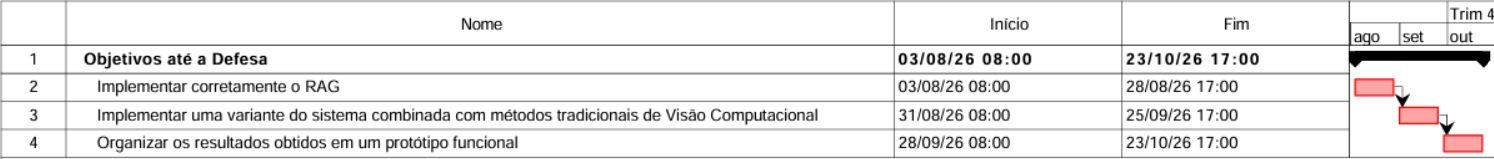
\includegraphics[width=1\textwidth]{imagens/Cronograma.png}}
\caption{Cronograma de execução das atividades do mestrado.}
\label{fig:crono}
\end{figure}
% % ----------------------------------------------------------
% % Referências bibliográficas
% % ----------------------------------------------------------
\renewcommand{\bibname}{REFERÊNCIAS}

\citeoption{abnt-full-initials=yes}

\bibliography{abntex2-modelo-references}
% % ----------------------------------------------------------
% % Glossário
% % ----------------------------------------------------------
% %
% % Consulte o manual da classe abntex2 para orientações sobre o glossário.
% %
% %\glossary


% % ----------------------------------------------------------
% % Apêndices
% % ----------------------------------------------------------
% % Inicia os apêndices
% % ---
% %\begin{apendicesenv}

% % Imprime uma página indicando o início dos apêndices
% %\partapendices


% %\include{apendice}

% %\end{apendicesenv}
% % ---


% \apendices
% %%% A linha abaixo impede que as seções, subseções, etc. dos apêndices e anexos
% %%% sejam mostradas no Sumário.
% \addtocontents{toc}{\protect\setcounter{tocdepth}{0}}

% %\renewcommand{\apendicesname}{APÊNDICES}
% %\partapendices*
% % --------------------------------------------------------------------
% \settocpreprocessor{chapter}{}
% \include{tex/appendices}


%--------------------------------------------------

% INDICE REMISSIVO
%---------------------------------------------------------------------
\phantompart

%---------------------------------------------------------------------


\end{document}